% =====================================================================
%  Software Requirements Specification (SRS) --- Leodega
%  Storage Marketplace
%
%  Institution : Escuela Superior Politecnica del Litoral (ESPOL)
%  Faculty     : Facultad de Ingenieria en Electricidad y Computacion (FIEC)
%  Course      : Software Engineering Isadasdsa
%
%  Sources of truth (in priority order):\input{seccion3_project_planning}
%     1. user_stories.md        (primary, functional requirements)
%     2. project_description.md (context, NFRs, technology stack)
%     3. previous_srs.md        (writing style reference only)
%  Structure authority: document_structure.md
%  Editorial rules:    instructions.md, prompt.md
%
%  Assumptions (flagged per instructions.md, item 5):
%     [A1] Course name: document_structure.md states "Software Engineering I"
%          while project_description.md states "Software Engineering II".
%          The value from document_structure.md (the required structure) is
%          used. Confirm with the professor.
%     [A2] Date and semester are left blank in document_structure.md.
%          "June 2026" is taken from the working environment date
%          (2026-06-22) and "PAO II - 2026" is inferred from the ESPOL
%          academic calendar (PAO II runs May--Aug). Confirm with ESPOL.
%     [A3] The ESPOL logo file is not present in the repository. A framed
%          placeholder is rendered automatically via \IfFileExists; place
%          "espol_logo.png" (and optionally "fiec_logo.png") in the
%          ./figures/ directory to embed the official marks.
% =====================================================================
\documentclass[11pt,a4paper,oneside]{report}

% ---- Encoding, font encoding, language --------------------------------
\usepackage[utf8]{inputenc}
\usepackage[T1]{fontenc}
\usepackage[english]{babel}

% ---- Page geometry ----------------------------------------------------
\usepackage[
    a4paper,
    top=2.5cm,
    bottom=2.5cm,
    left=2.5cm,
    right=2.5cm
]{geometry}

% ---- Typography -------------------------------------------------------
%   The default Computer Modern family is used so the document compiles
%   on a stock TeX Live installation without extra font packages.
%   microtype's font *expansion* requires scalable fonts, which the
%   bitmapped EC fonts are not; expansion is therefore disabled and only
%   protrusion (compatible with bitmapped fonts) is kept.
\usepackage[expansion=false]{microtype}
\usepackage{setspace}
\onehalfspacing

% Allow TeX to stretch interword space slightly to avoid overfull boxes
% caused by long, unbreakable technical terms (e.g. compound identifiers).
\emergencystretch=3em

% ---- Graphics ---------------------------------------------------------
\usepackage{graphicx}
\usepackage{float}
\graphicspath{{./figures/}{./ImgMeets/}{./}}

% ---- Color, rules, drawing --------------------------------------------
\usepackage{xcolor}
\usepackage{tikz}

% ---- Tables -----------------------------------------------------------
\usepackage{array}
\usepackage{booktabs}
\usepackage{tabularx}
\usepackage{longtable}
\newcolumntype{Y}{>{\raggedright\arraybackslash}X}

% ---- Lists and captions ----------------------------------------------
%   enumitem is not installed in this TeX Live; loaded conditionally so
%   the document still compiles and benefits from it when present.
\IfFileExists{enumitem.sty}{\usepackage{enumitem}\setlist{itemsep=2pt,parsep=0pt,topsep=4pt}}{}
\usepackage[font=small,labelfont=bf]{caption}

% ---- Headings ---------------------------------------------------------
%   titlesec is not installed in this TeX Live; loaded conditionally.
\IfFileExists{titlesec.sty}{\usepackage{titlesec}}{}

% ---- Headers and footers ---------------------------------------------
\usepackage{fancyhdr}

% ---- Hyperref (loaded late on purpose) --------------------------------
\usepackage[
    hidelinks,
    bookmarksnumbered=true,
    pdftitle={Software Requirements Specification --- Leodega},
    pdfauthor={Darwin Leonardo Diaz Gonzalez; Geovanny Jahir Diaz Loor; Carla Alejandra Gutierrez Cordova; Johao Carlos Dorado Quinde},
    pdfsubject={Software Requirements Specification},
    pdfkeywords={SRS, Leodega, Storage Marketplace, ESPOL, FIEC}
]{hyperref}

% ---- Document information --------------------------------------------
\newcommand{\DocTitle}{Software Requirements Specification}
\newcommand{\ProjectName}{Leodega}
\newcommand{\ProjectTagline}{Storage Marketplace}

\begin{document}

% =====================================================================
%  FRONT PAGE
%  (follows the ESPOL institutional format as specified in
%   document_structure.md, section "Front Page")
% =====================================================================
\begin{titlepage}
    \centering
    \thispagestyle{empty}
    \begin{spacing}{1}% single spacing keeps the cover on one page

    \vspace*{0.2cm}

    % --- Institutional header: logos ----------------------------------
    %   ESPOL logo (primary).  FIEC logo is shown alongside when present.
    %   See assumption [A3] in the file header.
    \IfFileExists{espol_logo.png}{%
        
\includegraphics[height=2.6cm,keepaspectratio]{espol_logo.png}%
    }{%
        \fbox{\parbox[c][2.6cm][c]{3.6cm}{\centering\bfseries ESPOL\\[2pt]\scriptsize\itshape (logo placeholder)}}%
    }%
    \hspace{0.8cm}%
    \IfFileExists{fiec_logo.png}{%
        \includegraphics[height=2.6cm,keepaspectratio]{fiec_logo.png}%
    }{}%
    \\[0.5cm]

    % --- University and faculty names ---------------------------------
    {\Large\bfseries Escuela Superior Politecnica del Litoral}\\[0.2cm]
    {\large\bfseries Facultad de Ingenieria en Electricidad y Computacion}\\[1.0cm]

    % --- Course -------------------------------------------------------
    {\large Software Engineering I}\\[1.0cm]

    % --- Project title block ------------------------------------------
    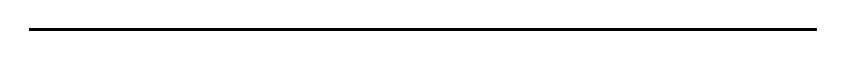
\begin{tikzpicture}
        \draw[line width=1.2pt] (-5,0) -- (5,0);
    \end{tikzpicture}\\[0.3cm]
    {\Huge\bfseries \ProjectName}\\[0.2cm]
    {\large\itshape \ProjectTagline}\\[0.3cm]
    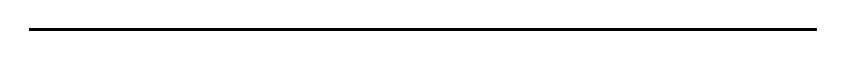
\begin{tikzpicture}
        \draw[line width=1.2pt] (-5,0) -- (5,0);
    \end{tikzpicture}\\[1.0cm]

    % --- Document descriptor ------------------------------------------
    {\large\bfseries \DocTitle}\\[1.1cm]

    % --- Team members -------------------------------------------------
    {\large\bfseries Team Members}\\[0.3cm]
    \begin{tabular}{c}
        Darwin Leonardo D\'iaz Gonz\'alez \\
        Geovanny Jahir Diaz Loor \\
        Carla Alejandra Guti\'errez C\'ordova \\
        Johao Carlos Dorado Quinde \\
    \end{tabular}\\[1.1cm]

    % --- Professor ----------------------------------------------------
    {\large\bfseries Professor}\\[0.3cm]
    {Mgti. Vanessa Jurado Alexandra Vite}\\[1.2cm]

    % --- Date and semester (see assumption [A2]) ----------------------
    {\large June 2026}\\[0.2cm]
    {\normalsize PAO II -- 2026}

    \end{spacing}
    \vfill
\end{titlepage}

\tableofcontents
\newpage

\listoffigures
\newpage

\listoftables
\newpage
% =====================================================================
%  1. INTRODUCTION
%  (document_structure.md, section "1. Introduction")
%
%  Sources used in this chapter:
%    * project_description.md  -> inherited start state supplied by the
%      product owner (technology stack, existing capabilities, business
%      goals, target users, business rules, known issues).
%    * user_stories.md         -> primary source for the functional
%      scope (epics HUG, HUC, HUA, HUE, HUL).
%    * document_structure.md   -> required subsections 1.1--1.5.
%
%  Additional assumptions flagged here:
%     [A4] Terminology: user_stories.md names the roles "Storage Manager",
%          "Client", "Administrator", "Organization Administrator", and
%          the mobile companion "Leodeguita". project_description.md
%          names them "landlord", "tenant", and "System Administrator".
%          Because user stories are the primary source, the user-story
%          terms are adopted as canonical and mapped to the inherited
%          codebase terms once, in Section 1.2.
%     [A5] The "Leodeguita" mobile companion is in scope (HUL-01..HUL-06).
%          project_description.md states a React Native app is "planned
%          for future versions"; the technology is therefore assumed to
%          be React Native, but only the six Leodeguita flows are
%          required by this specification.
% =====================================================================
\chapter{Introduction}

% ---------------------------------------------------------------------
\section{Problem Definition}
% ---------------------------------------------------------------------

The storage of goods is a recurring logistical need for both individuals and companies, yet the available supply of storage space is fragmented and largely underutilised. Many property owners hold unused spaces --- warehouses, garages, rooms, containers, basements, and attics --- that could be offered to third parties, while many other individuals and organisations struggle to find flexible, adequately sized, and conveniently located storage alternatives. At present, the matching between supply and demand of storage space is mostly carried out through informal, unmediated channels, which makes the process slow, opaque, and risky for both parties.

This situation gives rise to several concrete problems that the present software project intends to solve:

\begin{itemize}
    \item \textbf{Lack of trust and verifiable information.} Prospective renters cannot easily verify the conditions, dimensions, location, or legal compliance of a storage space before committing to a rental, and owners lack a structured reputation mechanism to demonstrate reliability.
    \item \textbf{Absence of formal moderation and compliance control.} There is no centralised authority that validates listings --- for example, that the mandatory fire department permit is in order --- before they are exposed to the public.
    \item \textbf{Inefficient reservation and contracting.} The coordination of availability windows, the detection of date conflicts, the formalisation of payment, and the activation of contracts are performed manually, which is error-prone and does not scale.
    \item \textbf{Limited communication and incident management.} Once a rental begins, the parties lack a dedicated channel to coordinate access, resolve incidents, or escalate problems to a moderator, and there is no structured report-and-resolution workflow.
    \item \textbf{No support for organisational (company-level) rentals.} Companies that need storage space for their collaborators cannot manage rentals under a collective identity, invite members, or audit the actions performed in the organisation's name.
    \item \textbf{No mobile access.} The management of published spaces and the exploration of available spaces are confined to a web experience, which limits on-the-go use by owners and clients.
    \item \textbf{No integration with external inventory systems.} Clients who already manage their stock in an external system must re-enter their product data manually, with no mechanism to query or import inventory automatically.
\end{itemize}

To address these problems, the product owner supplied an existing web platform, \textbf{Leodega}, as the starting point of the project. This platform already provides a collaborative marketplace for storage space --- including listing publication, search, reservations, ratings, reports, moderation, notifications, and messaging --- but it must be extended with the organisational, mobile, integration, compliance, and control capabilities specified in the user stories, which constitute the primary source of functional requirements for this document.

% ---------------------------------------------------------------------
\section{Project Context}
% ---------------------------------------------------------------------

The product owner provided the team with an existing full-stack web application, \textbf{Leodega}, as the start state of the project. Leodega is an online marketplace that connects \emph{landlords} (storage owners, hereafter \emph{Storage Managers}) with \emph{tenants} (renters, hereafter \emph{Clients}), and is overseen by a \emph{System Administrator}. At the moment of delivery, the platform was in the integration and testing phase and had been developed under the Scrum methodology.

The inherited platform is implemented with the following technology base, which constitutes the foundation on which the requirements specified in this document are built:

\begin{itemize}
    \item \textbf{Backend.} Laravel~12 (PHP~8.2+) with Laravel Sanctum token-based authentication, Eloquent ORM, and a PostgreSQL database in production (SQLite in local development), containerised with Docker Compose and deployable to Railway.
    \item \textbf{Frontend.} React~19 with TypeScript and Vite, React Router DOM with protected and role-based route guards, Tailwind CSS, Axios with a Bearer-token interceptor, Leaflet/React-Leaflet maps, and i18next internationalisation; deployable to Vercel.
    \item \textbf{Existing capabilities.} User authentication and registration, role-based access control (administrator, landlord, tenant), publication and moderation of storage spaces, search and detail views, reservations with conflict detection, ratings, reports, in-app notifications, conversations and messages, a payments registry, and role-based dashboards.
\end{itemize}

The team's task is to evolve this inherited platform so that it satisfies the functional requirements expressed in the user stories, extending it with organisational accounts, a mobile companion named \emph{Leodeguita}, external inventory integration, Excel inventory import, fire-department-permit compliance, an administrative control dashboard, and account moderation. The system operates in a web environment and requires an Internet connection; the Leodeguita companion extends the principal functions to mobile devices.

% ---------------------------------------------------------------------
\section{General Objective}
% ---------------------------------------------------------------------

To evolve the Leodega platform into a complete, reliable, and mobile-accessible storage marketplace that connects Storage Managers and Clients --- individually or under organisations --- through a moderated and trustworthy system that integrates reservation, payment, communication, incident-reporting, and inventory-integration capabilities, as specified in the user stories.

% ---------------------------------------------------------------------
\section{Specific Objectives}
% ---------------------------------------------------------------------

The following specific objectives support the general objective and correspond to the functional-requirement groups defined in the user stories:

\begin{enumerate}
    \item \textbf{Storage management.} Enable Storage Managers to register, edit, and delete warehouses --- including the mandatory fire department permit --- and to view, cancel, and communicate about their reservations. (References: HUG-01 to HUG-08.)
    \item \textbf{Client experience.} Enable Clients to search and filter warehouses, view their details, reserve and pay for them, manage their reservations, communicate with managers, report incidents, rate finished rentals, and integrate their external inventory systems or import inventory from Excel files. (References: HUC-01 to HUC-14.)
    \item \textbf{Platform administration.} Enable Administrators to validate fire department permits and moderate listings, block and reactivate user accounts, monitor a control dashboard with key metrics, and review and resolve reports. (References: HUA-01 to HUA-04.)
    \item \textbf{Organisational accounts.} Enable the creation of organisations, the invitation and acceptance of client members, the switching between personal and organisation contexts, business-level reservations, and the administration and auditing of organisational activity. (References: HUE-01 to HUE-06.)
    \item \textbf{Mobile companion (Leodeguita).} Provide mobile access for authentication with Leodega credentials, company selection, warehouse publication, and browsing of available warehouses. (References: HUL-01 to HUL-06.)
\end{enumerate}

% ---------------------------------------------------------------------
\section{Project Scope}
% ---------------------------------------------------------------------

The scope of the system is defined by the functional requirements derived from the user stories, which are summarised in Chapter~2 and detailed in Appendix~A. The inherited Leodega platform provides the technological and functional foundation described in Section~1.2; the present specification governs the capabilities that the delivered system must satisfy.

\subsection*{Functional scope by user level}

\textbf{Storage Manager (landlord).} The system allows the Storage Manager to: receive and reply to pre-booking inquiries; receive payment-confirmation notifications and view active contracts; chat with clients during active rentals; register a warehouse with dimensions, location, photos, monthly rate, and fire department permit; view reservations with filtering and detail; cancel future paid reservations with a mandatory reason; delete warehouses that have no active or future reservations; and edit warehouse information. (HUG-01 to HUG-08.)

\textbf{Client (tenant).} The system allows the Client to: search and filter warehouses by location, size, and price, with a map view; view warehouse details; reserve available warehouses with date-conflict validation; complete a simulated payment to confirm a reservation; communicate with managers before and during rentals; view and manage active and historical reservations; cancel future confirmed reservations; report incidents; rate finished rentals; accept or reject organisation invitations; register an external inventory endpoint and its field mapping; view synchronised inventory; and import inventory from an Excel file. (HUC-01 to HUC-14.)

\textbf{Administrator.} The system allows the Administrator to: validate the fire department permit and approve or reject warehouse publications; block and reactivate user accounts with audit logging; monitor a control dashboard with warehouse, user, transaction, reservation, and unresolved-report metrics; and review, reply to, and resolve reports. (HUA-01 to HUA-04.)

\textbf{Organisation Administrator and organisation members.} The system allows an Organisation Administrator to: create an organisation; invite clients as members; access a business administrative panel with members, reservations, and history; and delete business reservations with a mandatory reason. It allows member clients to: switch between personal and organisation contexts; reserve on behalf of the organisation; and share visibility of business reservations, while being prevented from deleting business reservations. (HUE-01 to HUE-06.)

\textbf{Leodeguita users (all roles).} The mobile companion allows any Leodega user to authenticate with existing credentials; allows a client to select the operating company; allows a Storage Manager to publish a warehouse for review and to view their published warehouses; and allows a client to browse and view the detail of available warehouses. (HUL-01 to HUL-06.)

\subsection*{Out of scope}

The following items are explicitly out of scope of this specification:

\begin{itemize}
    \item \textbf{Real financial payment processing.} The payment flow is simulated (HUC-05); integration with real payment gateways or banking processors is not required.
    \item \textbf{ERP integration and electronic invoicing.} These are part of the project vision but are not yet implemented and are not covered by any user story; they are excluded from this specification.
    \item \textbf{A general-purpose React Native mobile application.} A full mobile application is planned for future versions; only the Leodeguita companion flows specified in HUL-01 to HUL-06 are in scope.
    \item \textbf{Inherited-baseline features not re-specified in the user stories} (for example, favourites, session-token management, and password reset) are retained from the inherited platform as-is and are not re-specified as functional requirements in this document.
\end{itemize}

% =====================================================================
%  2. REQUIREMENTS SUMMARY
%  (document_structure.md, section "2. Requirements Summary")
%
%  2.1 Functional Requirements:
%      Summary table of IDs, names, and references to the detailed
%      User Stories in Appendix A. The source of every functional
%      requirement is user_stories.md (primary source per
%      instructions.md, item 6). Story IDs are preserved verbatim
%      (HUG, HUC, HUA, HUE, HUL prefixes) so they match the appendix
%      and the team's backlog.
%
%  2.2 Non-Functional Requirements:
%      Summary table categorised according to Ian Sommerville's
%      classification (Product, Organisational, External) as required
%      by document_structure.md and instructions.md, item 13. Detailed
%      statements and validation criteria live in Appendix B and are
%      sourced from non_functional_requierements.md.
% =====================================================================
\chapter{Requirements Summary}

This chapter consolidates the functional and non-functional requirements of the Leodega platform in summary form. The functional requirements are expressed as User Stories and are detailed in Appendix~A; the non-functional requirements are detailed in Appendix~B. The summaries presented here provide a quick, traceable overview and do not replace the detailed specifications given in the appendices.

% ---------------------------------------------------------------------
\section{Functional Requirements}
% ---------------------------------------------------------------------

The functional requirements of the system are derived exclusively from the User Stories supplied in \texttt{user\_stories.md}, which constitute the primary source of functional requirements per the editorial instructions. They are organised by the five roles that interact with the system: \textbf{Storage Manager} (HUG), \textbf{Client} (HUC), \textbf{Administrator} (HUA), \textbf{Organisation / Company} (HUE), and the \textbf{Leodeguita} mobile companion (HUL). Table~\ref{tab:fr-summary} lists every requirement by ID, a concise descriptive name, and the reference to its detailed User Story in Appendix~A.

\begin{longtable}{>{\raggedright\arraybackslash}p{2.0cm} p{9.2cm} >{\raggedright\arraybackslash}p{3.4cm}}
    \caption{Functional Requirements Summary} \label{tab:fr-summary} \\
    \toprule
    \textbf{ID} & \textbf{Requirement Name} & \textbf{Reference} \\
    \midrule
    \endfirsthead

    \multicolumn{3}{c}{\itshape Table~\ref{tab:fr-summary} (continued)} \\
    \midrule
    \textbf{ID} & \textbf{Requirement Name} & \textbf{Reference} \\
    \midrule
    \endhead

    \midrule
    \multicolumn{3}{r}{\itshape continued on next page} \\
    \endfoot

    \bottomrule
    \endlastfoot

    % --- Storage Manager (HUG) ---
    \multicolumn{3}{l}{\textit{Storage Manager (HUG)}} \\
    \midrule
    HUG-01 & Pre-booking inquiry reception and reply & App.~A, HUG-01 \\
    HUG-02 & Payment-confirmation notification and contract activation & App.~A, HUG-02 \\
    HUG-03 & Active-contract chat with clients & App.~A, HUG-03 \\
    HUG-04 & Warehouse registration with fire department permit & App.~A, HUG-04 \\
    HUG-05 & Reservation list viewing, filtering, and detail & App.~A, HUG-05 \\
    HUG-06 & Cancellation of paid future reservations & App.~A, HUG-06 \\
    HUG-07 & Warehouse deletion (no active or future reservations) & App.~A, HUG-07 \\
    HUG-08 & Warehouse information editing & App.~A, HUG-08 \\
    \midrule

    % --- Client (HUC) ---
    \multicolumn{3}{l}{\textit{Client (HUC)}} \\
    \midrule
    HUC-01 & Warehouse search, filtering, and map view & App.~A, HUC-01 \\
    HUC-02 & Warehouse detail view & App.~A, HUC-02 \\
    HUC-03 & Warehouse reservation with date-conflict detection & App.~A, HUC-03 \\
    HUC-04 & Pre-booking message to manager & App.~A, HUC-04 \\
    HUC-05 & Simulated payment confirmation & App.~A, HUC-05 \\
    HUC-06 & Active-reservation chat & App.~A, HUC-06 \\
    HUC-07 & Reservation history management and cancellation & App.~A, HUC-07 \\
    HUC-08 & Incident reporting and tracking & App.~A, HUC-08 \\
    HUC-09 & Warehouse and manager rating and review & App.~A, HUC-09 \\
    HUC-10 & External inventory endpoint registration & App.~A, HUC-10 \\
    HUC-11 & External inventory field mapping & App.~A, HUC-11 \\
    HUC-12 & Synchronised inventory viewing & App.~A, HUC-12 \\
    HUC-13 & Excel inventory import & App.~A, HUC-13 \\
    HUC-14 & Organisation invitation acceptance or rejection & App.~A, HUC-14 \\
    \midrule

    % --- Administrator (HUA) ---
    \multicolumn{3}{l}{\textit{Administrator (HUA)}} \\
    \midrule
    HUA-01 & Fire department permit validation & App.~A, HUA-01 \\
    HUA-02 & Administrative control dashboard & App.~A, HUA-02 \\
    HUA-03 & User account blocking and reactivation & App.~A, HUA-03 \\
    HUA-04 & Report review and resolution & App.~A, HUA-04 \\
    \midrule

    % --- Organisation / Company (HUE) ---
    \multicolumn{3}{l}{\textit{Organisation / Company (HUE)}} \\
    \midrule
    HUE-01 & Organisation member invitation & App.~A, HUE-01 \\
    HUE-02 & Personal / organisation context switching & App.~A, HUE-02 \\
    HUE-03 & Business administrative panel & App.~A, HUE-03 \\
    HUE-04 & Organisation creation & App.~A, HUE-04 \\
    HUE-05 & Business-level reservation & App.~A, HUE-05 \\
    HUE-06 & Business reservation deletion control & App.~A, HUE-06 \\
    \midrule

    % --- Leodeguita (HUL) ---
    \multicolumn{3}{l}{\textit{Leodeguita mobile companion (HUL)}} \\
    \midrule
    HUL-01 & Leodeguita login with Leodega credentials & App.~A, HUL-01 \\
    HUL-02 & Company selection in Leodeguita & App.~A, HUL-02 \\
    HUL-03 & Mobile warehouse publication for review & App.~A, HUL-03 \\
    HUL-04 & Published warehouses list (mobile) & App.~A, HUL-04 \\
    HUL-05 & Available spaces browsing (mobile) & App.~A, HUL-05 \\
    HUL-06 & Warehouse detail view (mobile) & App.~A, HUL-06 \\
\end{longtable}

In total, the specification comprises 38 functional requirements: 8 for the Storage Manager, 14 for the Client, 4 for the Administrator, 6 for the Organisation, and 6 for the Leodeguita mobile companion. Each entry in Table~\ref{tab:fr-summary} is traceable to a User Story in Appendix~A, where the full statement, priority, estimate, sprint, and acceptance criteria are provided.

% ---------------------------------------------------------------------
\section{Non-Functional Requirements}
\label{sec:non-functional-requirements-summary}
% ---------------------------------------------------------------------

The non-functional requirements of the system are sourced from \texttt{non\_\allowbreak functional\_\allowbreak requierements.md} and are categorised according to Ian Sommerville's classification, which distinguishes three top-level families of quality requirements:

\begin{itemize}
    \item \textbf{Product requirements} constrain the behaviour of the software itself (e.g., efficiency, reliability, usability, security, portability).
    \item \textbf{Organisational requirements} arise from the policies, procedures, and development standards of the team and institution (e.g., implementation and process standards).
    \item \textbf{External requirements} arise from factors outside the system and its development, such as regulatory or legislative obligations.
\end{itemize}

Table~\ref{tab:nfr-summary} lists each non-functional requirement by ID, a concise name, its Sommerville category, and the reference to its detailed specification in Appendix~B, where the validation criteria are provided.

\begin{table}[h]
    \centering
    \caption{Non-Functional Requirements Summary (Sommerville classification)}
    \label{tab:nfr-summary}
    \begin{tabularx}{\textwidth}{>{\raggedright\arraybackslash}p{1.5cm} >{\raggedright\arraybackslash}X >{\raggedright\arraybackslash}p{4.0cm} >{\raggedright\arraybackslash}p{2.3cm}}
        \toprule
        \textbf{ID} & \textbf{Requirement Name} & \textbf{Sommerville Category} & \textbf{Reference} \\
        \midrule
        RNF-01 & Performance (response time)            & Product --- Efficiency            & App.~B, RNF-01 \\
        RNF-02 & Availability                            & Product --- Reliability           & App.~B, RNF-02 \\
        RNF-03 & Security: Authentication                & Product --- Security              & App.~B, RNF-03 \\
        RNF-04 & Security: Data protection               & Product --- Security              & App.~B, RNF-04 \\
        RNF-05 & Usability                               & Product --- Usability             & App.~B, RNF-05 \\
        RNF-06 & Compatibility (browsers and devices)    & Product --- Portability           & App.~B, RNF-06 \\
        RNF-07 & Internationalization                    & Product --- Portability           & App.~B, RNF-07 \\
        RNF-08 & Maintainability                         & Organisational --- Implementation & App.~B, RNF-08 \\
        RNF-09 & Testability                             & Organisational --- Implementation & App.~B, RNF-09 \\
        RNF-10 & Scalability                             & Product --- Efficiency            & App.~B, RNF-10 \\
        RNF-11 & Auditability                            & External --- Regulatory           & App.~B, RNF-11 \\
        \bottomrule
    \end{tabularx}
\end{table}

The categorisation in Table~\ref{tab:nfr-summary} follows Sommerville's framework: eight requirements (RNF-01, RNF-02, RNF-03, RNF-04, RNF-05, RNF-06, RNF-07, and RNF-10) constrain properties of the product; two requirements (RNF-08 and RNF-09) constrain the development process and its implementation standards; and one requirement (RNF-11) responds to external regulatory accountability needs through audit-trail traceability. Every non-functional requirement is stated in testable terms and is accompanied by quantitative validation criteria in Appendix~B, in compliance with the editorial instruction that every requirement be testable and that validation criteria be included for every non-functional requirement.

% =====================================================================
%  SECTION 3 - PROJECT PLANNING AND CONTROL  (Leodega)
%  STANDALONE DOCUMENT - compiles on its own.
%
%  Image files that must be in the same project/folder:
%   - AOA_Leodega_circulos.png                 (Figure 1)
%   - Resource_Limited_Leodega_1_.png          (Figure 2 - optimized)
%   - Resource_Limited_SinOptimizar_Leodega.png(Figure 3 - non-optimized)
% =====================================================================


\chapter{Project Planning and Control}

To plan and control the project, we first organized all the gathered requirements
(user stories) as individual tasks and defined their dependencies, prioritization
and sequencing across the five development sprints. After establishing all
requirements and their dependencies, we developed a Program Evaluation and Review
Technique (PERT) diagram, also known as an Activity-on-Arrow (AOA) diagram. This
diagram, shown in Figure~\ref{fig:aoa}, helps us schedule the project activities by
determining the earliest start times and required completion times for each event.
The diagram reveals a total project
duration of \textbf{52 time units (days)}, with the critical path highlighted in
red. The critical path runs through the activities
HST-001 $\rightarrow$ HST-002 $\rightarrow$ HST-007 $\rightarrow$ HST-009
$\rightarrow$ HST-011 $\rightarrow$ HST-013 $\rightarrow$ HST-014 $\rightarrow$
HST-034 $\rightarrow$ HST-035 $\rightarrow$ HST-036; that is, the chain that runs
from authentication and warehouse registration, through administrator moderation,
catalog search, warehouse detail, reservation and simulated payment, and ends with
the inventory-integration module (external connection, field mapping and inventory
view), which concentrates the heaviest tasks of the project (8, 8 and 5 days).

The project is structured into five sprints, each focusing on a specific aspect of
the platform's development:

\begin{itemize}
    \item \textbf{Sprint 1: Authentication and Warehouse Management Foundations}
    \begin{itemize}
        \item HST-001: Shared login for the web and the Leodeguita mobile app.
        \item HST-002: Warehouse registration including the fire-department permit.
        \item HST-003: Warehouse publishing from the mobile app.
        \item HST-004: Editing a published warehouse.
        \item HST-005: Logical deletion of a warehouse.
        \item HST-006: ``My warehouses'' listing (mobile).
        \item HST-007: Administrator moderation and approval of warehouses.
        \item HST-008: Blocking and reactivating user accounts.
    \end{itemize}
    \item \textbf{Sprint 2: Catalog, Reservations and Payment}
    \begin{itemize}
        \item HST-009: Search and filtering of approved warehouses.
        \item HST-010: Unified space listing (mobile).
        \item HST-011: Warehouse detail view.
        \item HST-012: Warehouse detail view (mobile).
        \item HST-013: Period reservation with temporary availability hold.
        \item HST-014: Simulated instant-book payment.
        \item HST-015: Payment-confirmation notification for the manager.
        \item HST-016: Manager reservation list.
        \item HST-017: Reservation cancellation by the manager.
    \end{itemize}
    \item \textbf{Sprint 3: Organizations (Multi-company)}
    \begin{itemize}
        \item HST-018: Organization creation from a client account.
        \item HST-019: Personal/organization context switcher.
        \item HST-020: Organization selector (mobile).
        \item HST-021: Inviting client users to the organization.
        \item HST-022: Accepting or rejecting invitations.
        \item HST-023: Organization administration panel.
        \item HST-024: Reserving on behalf of an organization.
        \item HST-025: Protection of organization reservations.
    \end{itemize}
    \item \textbf{Sprint 4: Messaging, Reports and Reviews}
    \begin{itemize}
        \item HST-026: Pre-booking inquiry (client side).
        \item HST-027: Pre-booking inquiry (manager side).
        \item HST-028: Reservation chat (client side).
        \item HST-029: Reservation chat (manager side).
        \item HST-030: Client reservation management.
        \item HST-031: Problem reporting.
        \item HST-032: Report management (administrator).
        \item HST-033: Rating and reviews.
    \end{itemize}
    \item \textbf{Sprint 5: Inventory Integration and Metrics}
    \begin{itemize}
        \item HST-034: External inventory connection (pull model).
        \item HST-035: Field mapping between the external system and Leodega.
        \item HST-036: On-demand inventory view.
        \item HST-037: Inventory import from an Excel file.
        \item HST-038: Administrator metrics dashboard.
    \end{itemize}
\end{itemize}

Based on our PERT analysis, we created the comprehensive schedule shown in
Table~\ref{tab:schedule}. This schedule details each requirement's sprint
assignment, predecessors, duration and resource allocation (staff), along with the
earliest event time (EET, i.e. the earliest start), the total float and the latest
event time (LET, i.e. the latest finish), all expressed in days. Activities whose
float is zero belong to the critical path and are marked with a bullet
($\bullet$). Note that HST-002 and HST-003 run in parallel and both have zero
float; the diagram draws the red critical path through HST-002.

\begin{figure}[h]
    \centering
    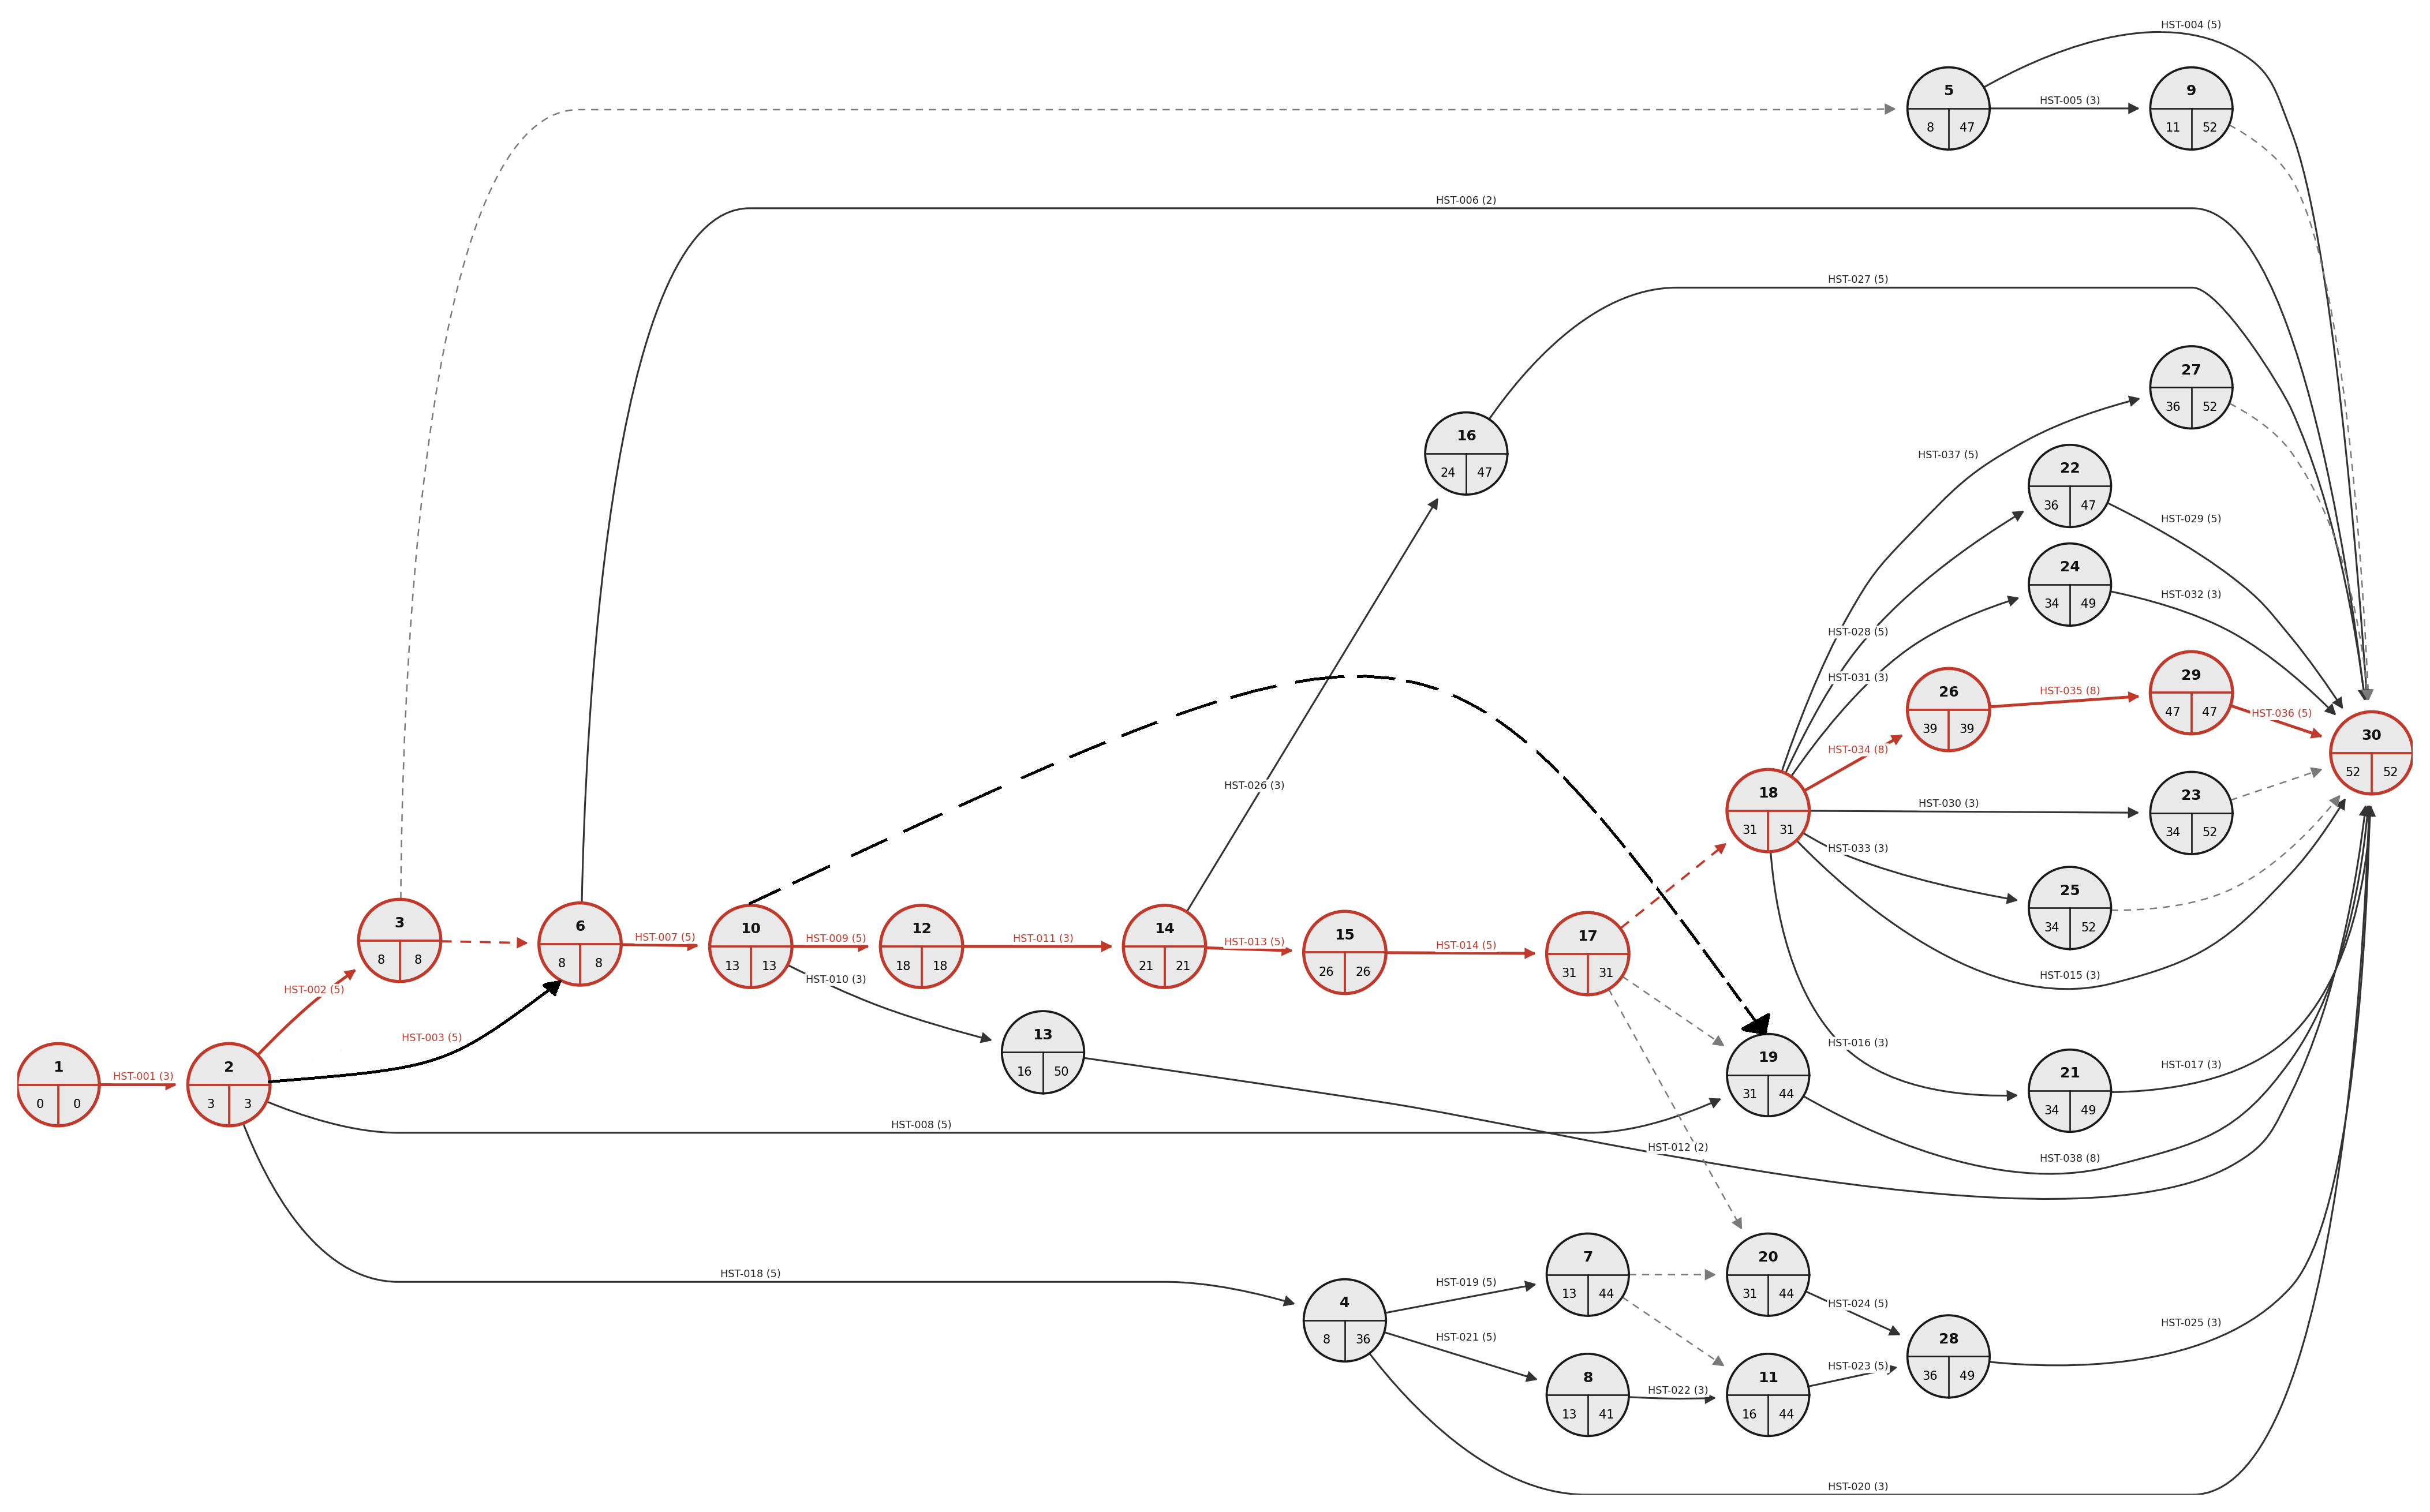
\includegraphics[width=\textwidth]{AOA_Leodega_circulos.png}
    \caption{Activity-on-Arrow (PERT) diagram for Leodega. The critical path is shown in red and the total project duration is 52 days.}
    \label{fig:aoa}
\end{figure}

\renewcommand{\arraystretch}{1.15}
\begin{longtable}{l c c c c c c c c}
\caption{Project schedule for Leodega: sprint, dependencies, timing, resource allocation and CPM analysis (EET, float, LET).}
\label{tab:schedule}\\
\toprule
\textbf{ID} & \textbf{Sprint} & \textbf{Pred.} & \textbf{Dur.} & \textbf{Staff} & \textbf{EET} & \textbf{Float} & \textbf{LET} & \textbf{CP}\\
\midrule
\endfirsthead

\multicolumn{9}{c}{\tablename\ \thetable\ -- \textit{continued from previous page}}\\
\toprule
\textbf{ID} & \textbf{Sprint} & \textbf{Pred.} & \textbf{Dur.} & \textbf{Staff} & \textbf{EET} & \textbf{Float} & \textbf{LET} & \textbf{CP}\\
\midrule
\endhead

\midrule
\multicolumn{9}{r}{\textit{continued on next page}}\\
\endfoot

\bottomrule
\endlastfoot

HST-001 & 1 & --            & 3 & 1 & 0  & 0  & 3  & $\bullet$\\
HST-002 & 1 & 001           & 5 & 2 & 3  & 0  & 8  & $\bullet$\\
HST-003 & 1 & 001           & 5 & 2 & 3  & 0  & 8  & $\bullet$\\
HST-004 & 1 & 002           & 5 & 2 & 8  & 39 & 52 & \\
HST-005 & 1 & 002           & 3 & 1 & 8  & 41 & 52 & \\
HST-006 & 1 & 002, 003      & 2 & 1 & 8  & 42 & 52 & \\
HST-007 & 1 & 002, 003      & 5 & 2 & 8  & 0  & 13 & $\bullet$\\
HST-008 & 1 & 001           & 5 & 2 & 3  & 36 & 44 & \\
HST-009 & 2 & 007           & 5 & 2 & 13 & 0  & 18 & $\bullet$\\
HST-010 & 2 & 007           & 3 & 1 & 13 & 34 & 50 & \\
HST-011 & 2 & 009           & 3 & 1 & 18 & 0  & 21 & $\bullet$\\
HST-012 & 2 & 010           & 2 & 1 & 16 & 34 & 52 & \\
HST-013 & 2 & 011           & 5 & 2 & 21 & 0  & 26 & $\bullet$\\
HST-014 & 2 & 013           & 5 & 2 & 26 & 0  & 31 & $\bullet$\\
HST-015 & 2 & 014           & 3 & 1 & 31 & 18 & 52 & \\
HST-016 & 2 & 014           & 3 & 1 & 31 & 15 & 49 & \\
HST-017 & 2 & 016           & 3 & 1 & 34 & 15 & 52 & \\
HST-018 & 3 & 001           & 5 & 2 & 3  & 28 & 36 & \\
HST-019 & 3 & 018           & 5 & 2 & 8  & 31 & 44 & \\
HST-020 & 3 & 018           & 3 & 1 & 8  & 41 & 52 & \\
HST-021 & 3 & 018           & 5 & 2 & 8  & 28 & 41 & \\
HST-022 & 3 & 021           & 3 & 1 & 13 & 28 & 44 & \\
HST-023 & 3 & 019, 022      & 5 & 2 & 16 & 23 & 49 & \\
HST-024 & 3 & 019, 014      & 5 & 2 & 31 & 13 & 49 & \\
HST-025 & 3 & 023, 024      & 3 & 1 & 36 & 13 & 52 & \\
HST-026 & 4 & 011           & 3 & 1 & 21 & 23 & 47 & \\
HST-027 & 4 & 026           & 5 & 2 & 24 & 23 & 52 & \\
HST-028 & 4 & 014           & 5 & 2 & 31 & 11 & 47 & \\
HST-029 & 4 & 028           & 5 & 2 & 36 & 11 & 52 & \\
HST-030 & 4 & 014           & 3 & 1 & 31 & 18 & 52 & \\
HST-031 & 4 & 014           & 3 & 1 & 31 & 15 & 49 & \\
HST-032 & 4 & 031           & 3 & 1 & 34 & 15 & 52 & \\
HST-033 & 4 & 014           & 3 & 1 & 31 & 18 & 52 & \\
HST-034 & 5 & 014           & 8 & 3 & 31 & 0  & 39 & $\bullet$\\
HST-035 & 5 & 034           & 8 & 3 & 39 & 0  & 47 & $\bullet$\\
HST-036 & 5 & 035           & 5 & 2 & 47 & 0  & 52 & $\bullet$\\
HST-037 & 5 & 014           & 5 & 2 & 31 & 16 & 52 & \\
HST-038 & 5 & 007, 008, 014 & 8 & 3 & 31 & 13 & 52 & \\
\end{longtable}

Because the critical-path duration of 52 days assumes unlimited resources, we then
performed resource-limited scheduling subject to a cap of four team members. We
first built a non-optimized schedule, shown in Figure~\ref{fig:rl-noopt}, which
completes the project in \textbf{87 days}. We then optimized it by levelling
resource usage and reordering non-critical activities within their available
float; the resulting optimized schedule, shown in Figure~\ref{fig:rl-opt},
completes the project in \textbf{85 days}. This optimization saves two days while
never exceeding the four-person limit and never delaying any critical activity.

\begin{figure}[H]
    \centering
    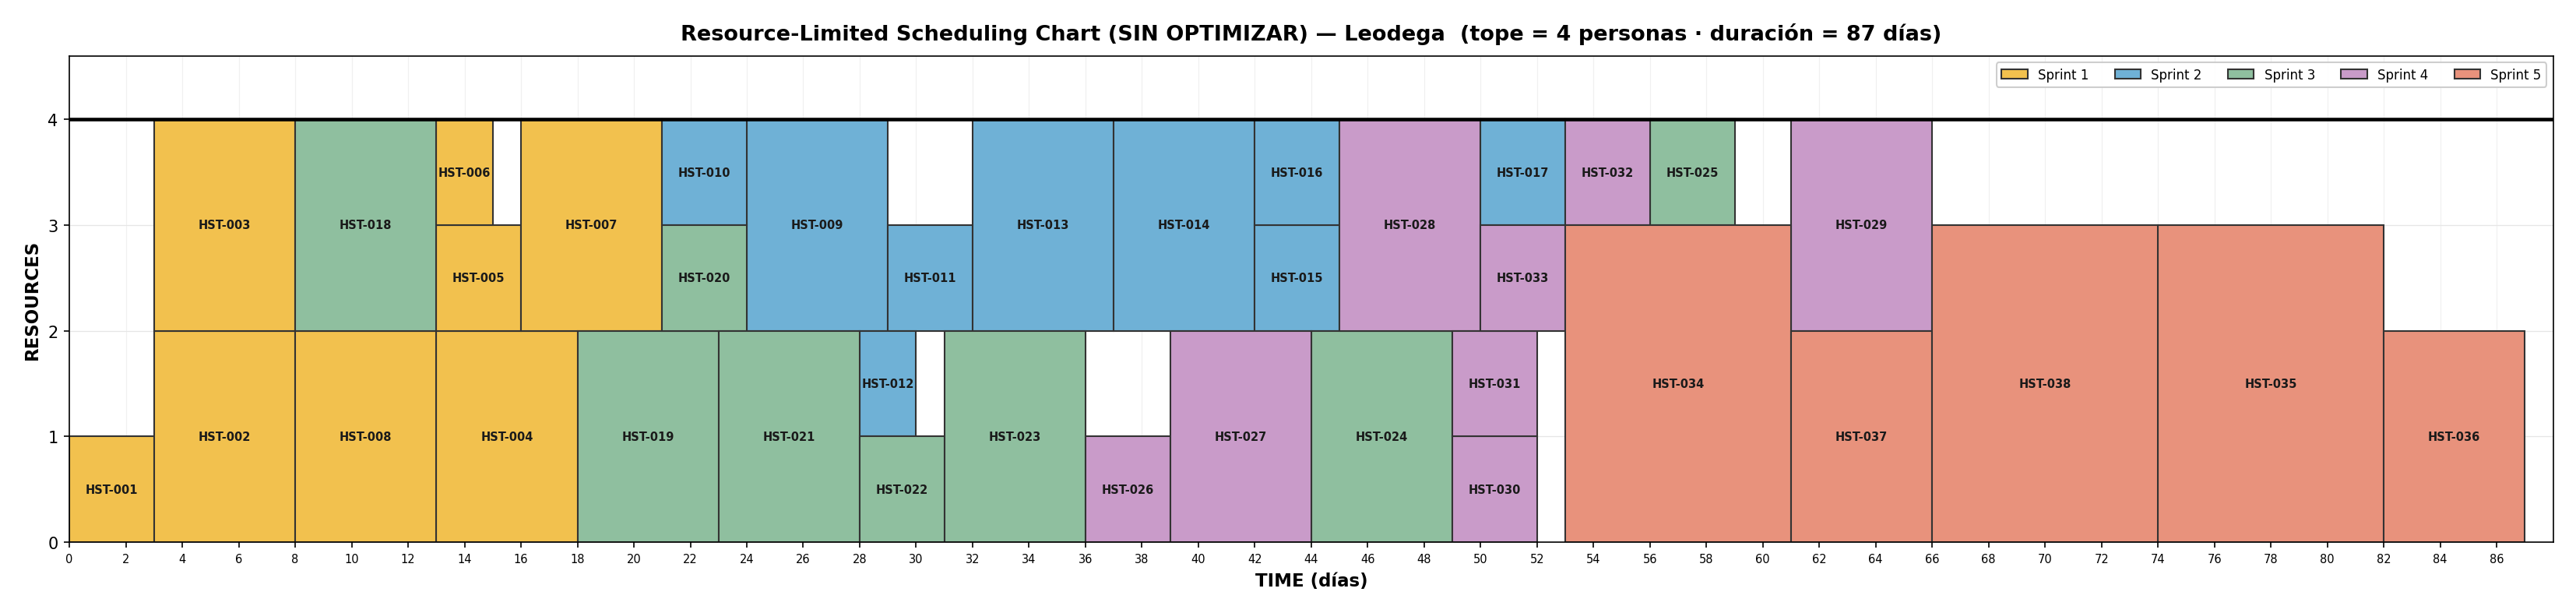
\includegraphics[width=\textwidth]{Resource_Limited_SinOptimizar_Leodega.png}
    \caption{Non-optimized resource-limited scheduling chart (cap = 4 people, total duration = 87 days).}
    \label{fig:rl-noopt}
\end{figure}

\begin{figure}[H]
    \centering
    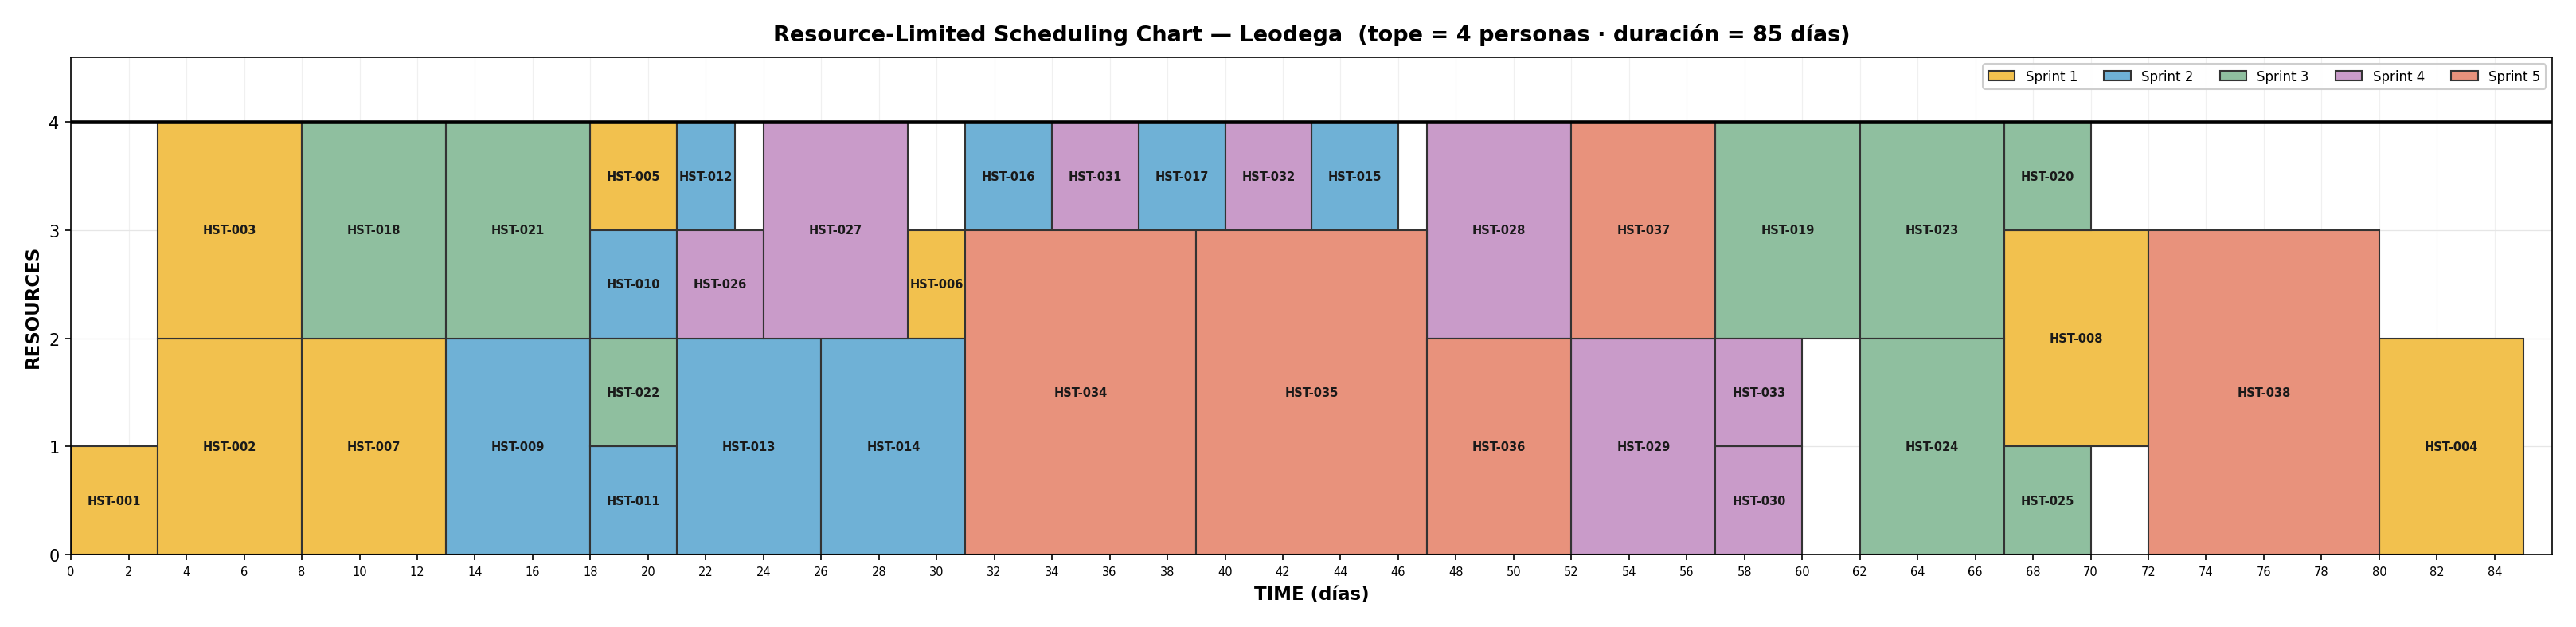
\includegraphics[width=\textwidth]{Resource_Limited_Leodega_1_.png}
    \caption{Optimized resource-limited scheduling chart (cap = 4 people, total duration = 85 days).}
    \label{fig:rl-opt}
\end{figure}

% ═══════════════════════════════════════════════════════════════════
%  CHAPTER 4 — SYSTEM PROTOTYPE (INTERFACE SCREENS)
%  Add \input{section4_prototype} BEFORE \chapter{Acceptance Letter}
%  Requires in preamble: \usepackage{graphicx}  \usepackage{float}
%  Images must be in the ./img/ folder in Overleaf.
% ═══════════════════════════════════════════════════════════════════

\chapter{System Prototype}
\label{chap:prototype-screens}

The Leodega prototype is a high-fidelity web application developed
using React and Tailwind CSS. The system supports three primary user
roles: \textbf{Tenant}, \textbf{Landlord/Manager}, and
\textbf{Administrator}, each with distinct interaction flows. The
following sections document the main screens of the prototype,
organised by user role.

% ───────────────────────────────────────────────────────────────────
\section{General Screens}
% ───────────────────────────────────────────────────────────────────

The following screens are shared across all user types, covering the
public landing page, authentication flow, and user profile selection.

\begin{figure}[H]
    \centering
    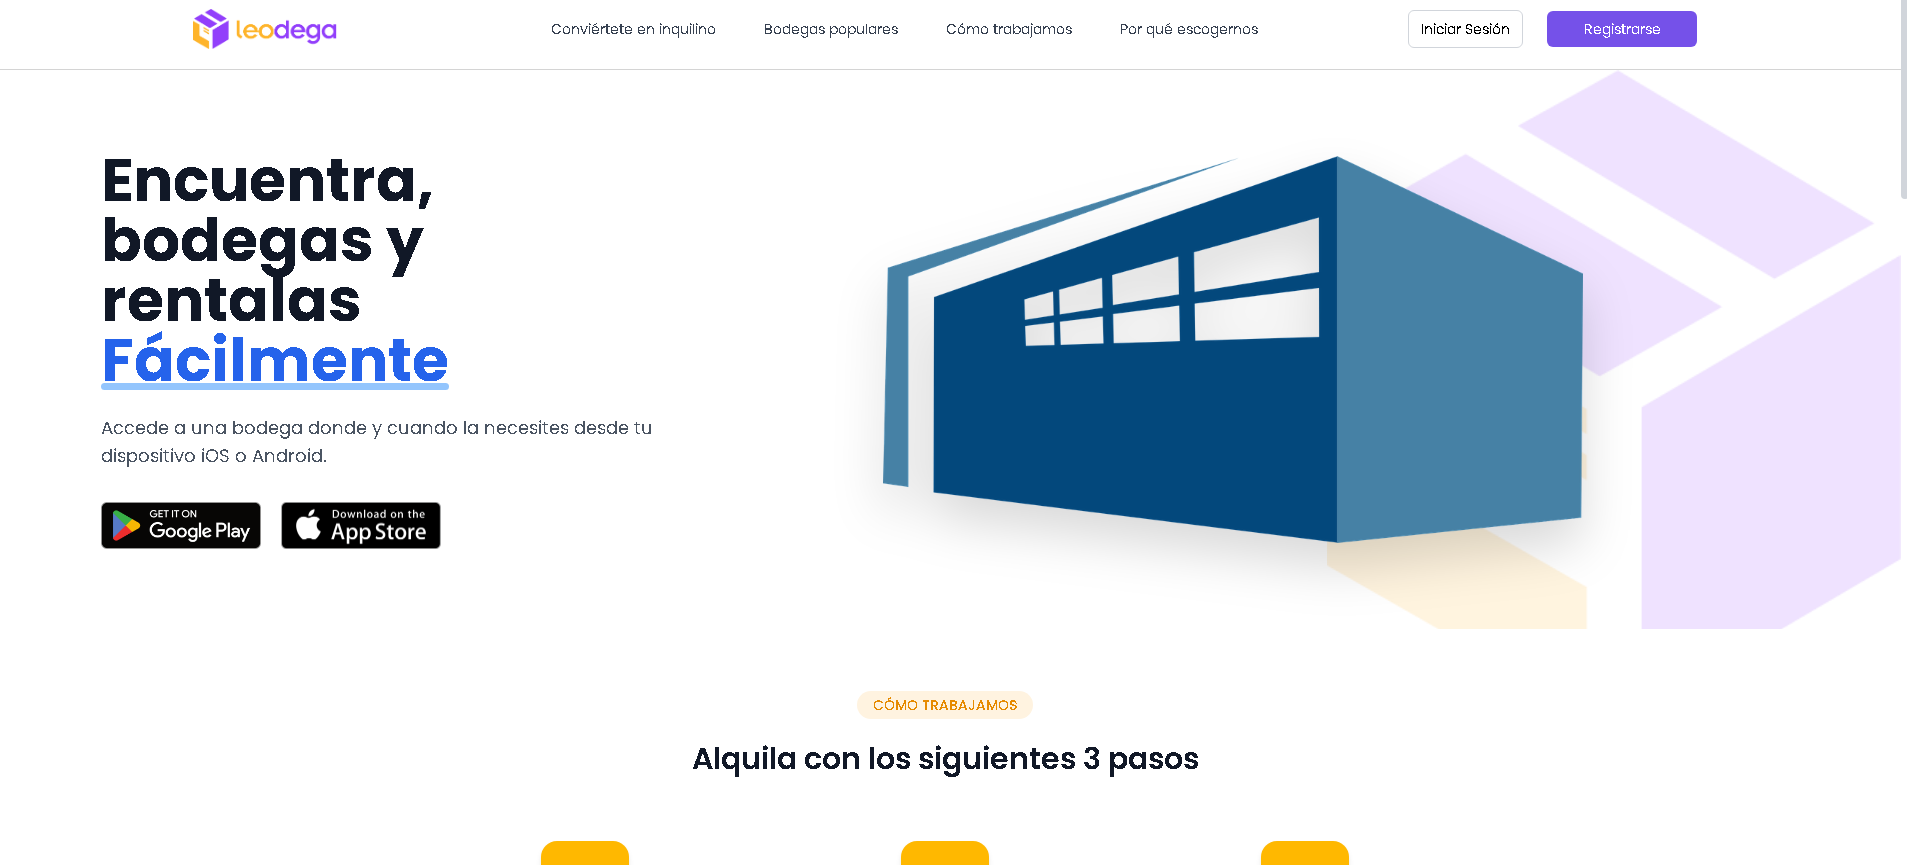
\includegraphics[width=\linewidth]{img/fig01_landing_hero}
    \caption{Landing Page: hero section with value proposition and
    mobile platform access links.}
    \label{fig:landing_hero}
\end{figure}

\begin{figure}[H]
    \centering
    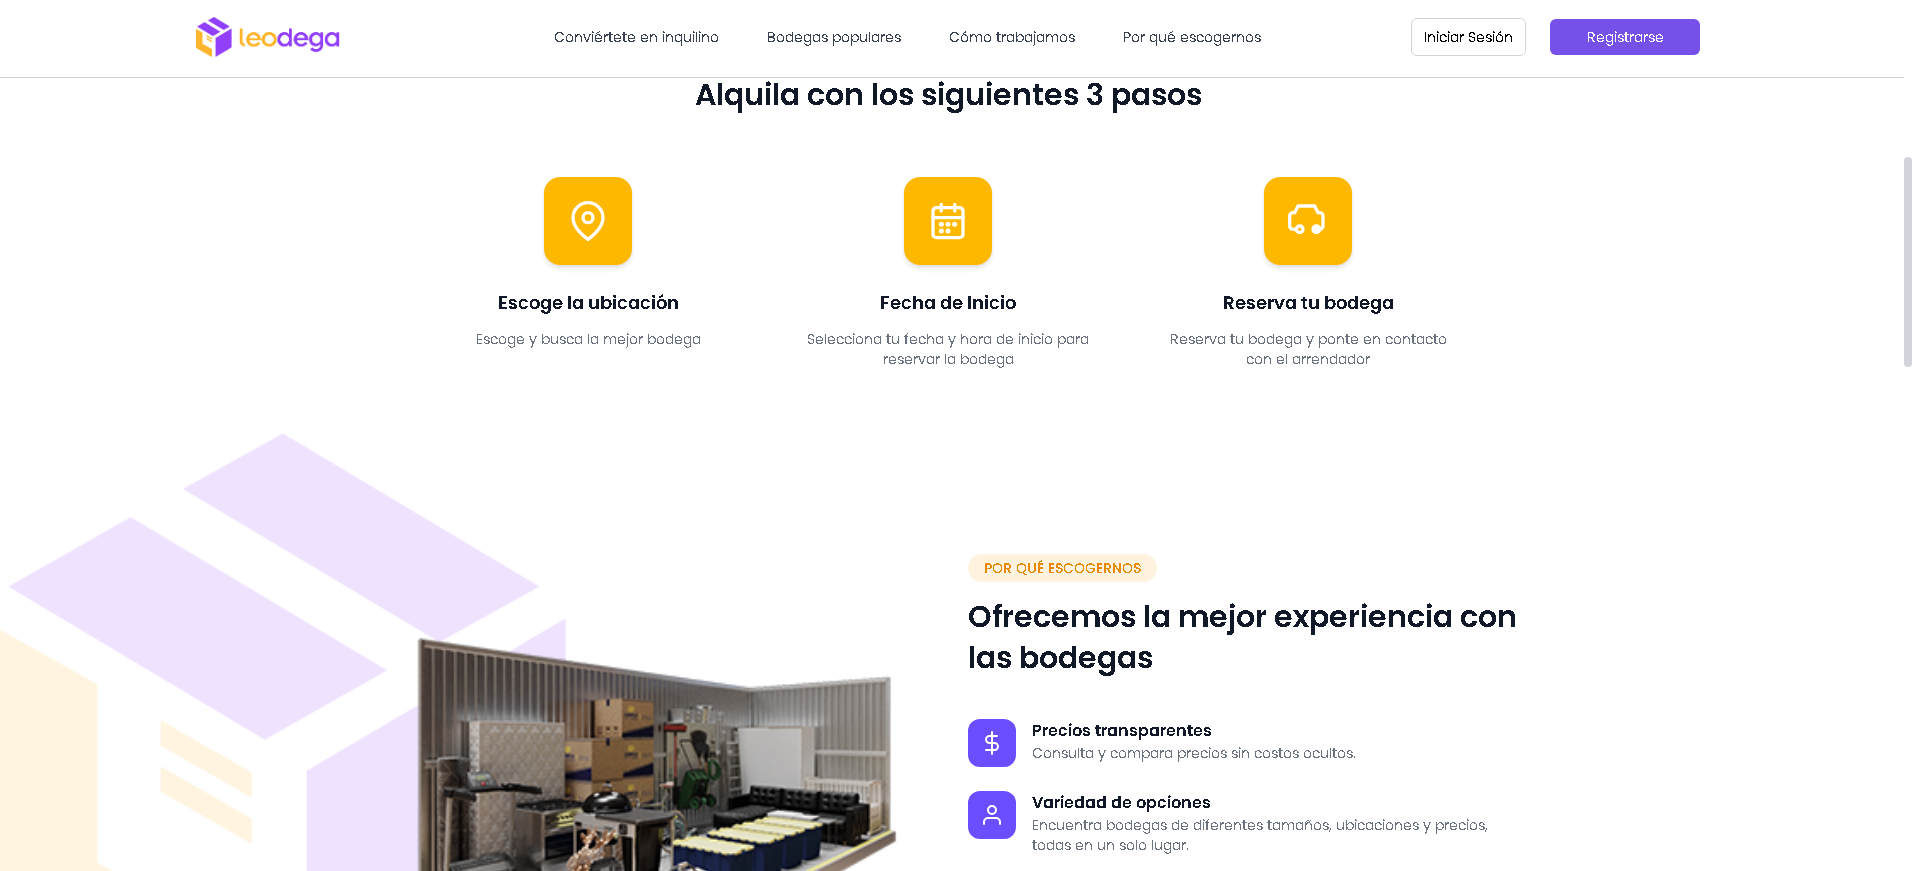
\includegraphics[width=\linewidth]{img/fig02_how_it_works}
    \caption{Landing Page: ``How We Work'' section presenting the
    warehouse rental process in three steps.}
    \label{fig:how_it_works}
\end{figure}

\begin{figure}[H]
    \centering
    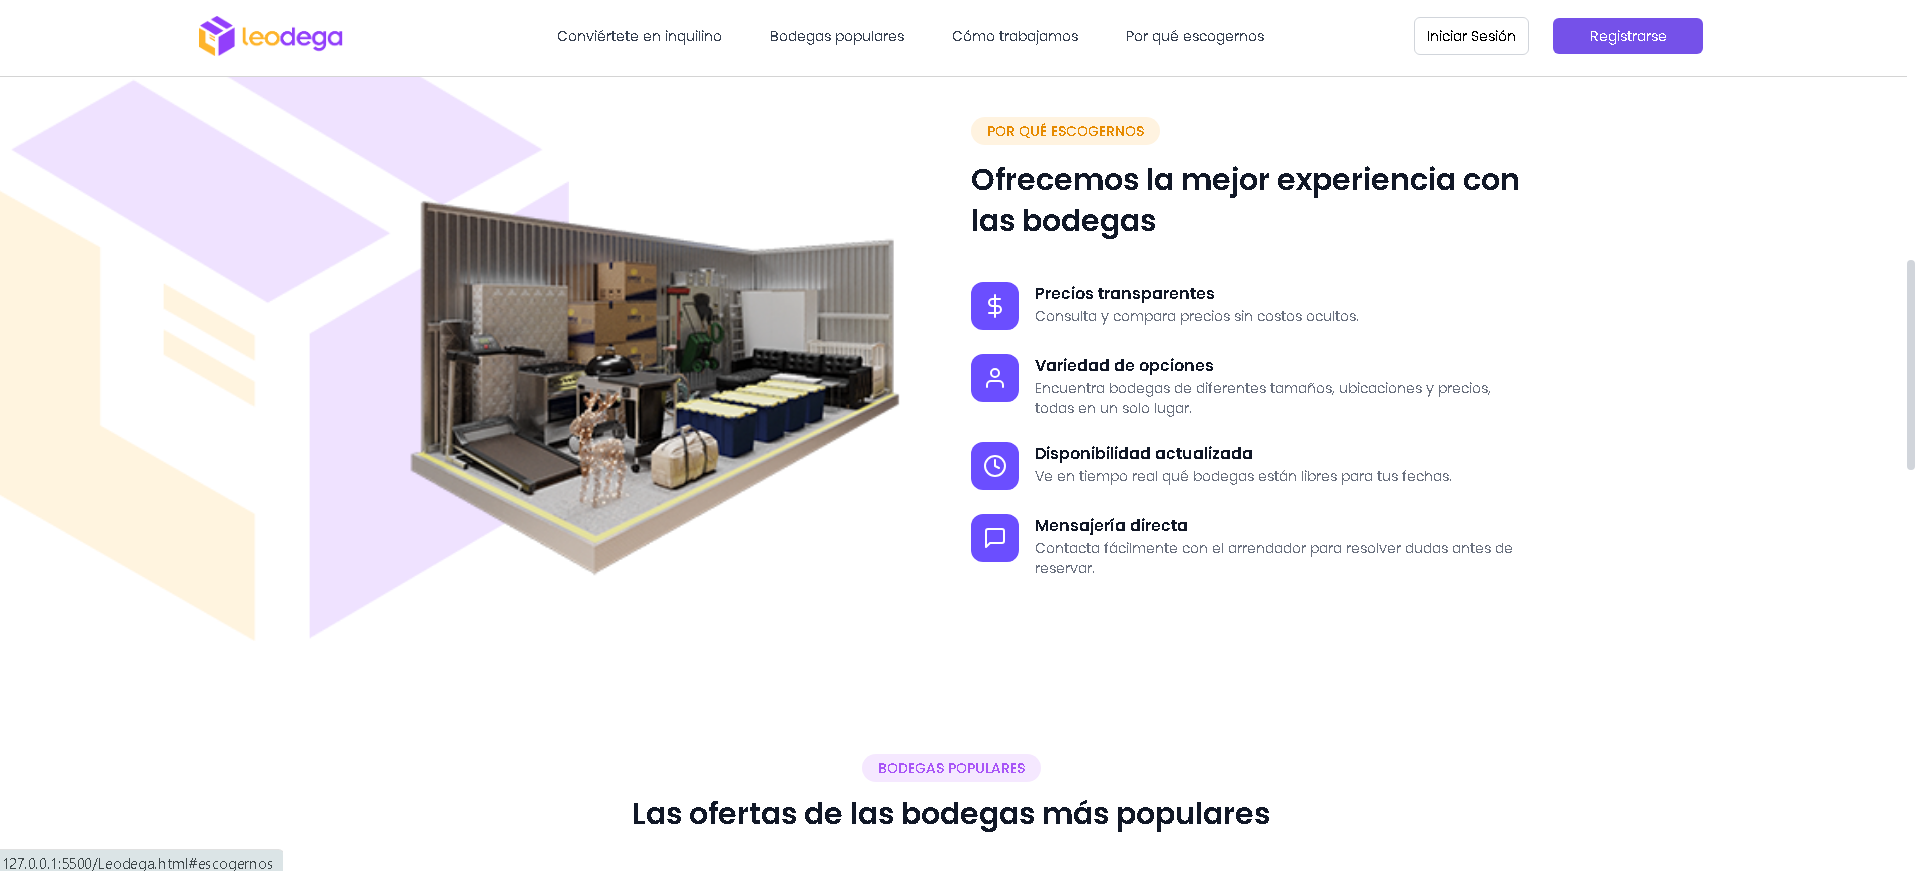
\includegraphics[width=\linewidth]{img/fig03_why_choose_us}
    \caption{Landing Page: ``Why Choose Us'' section highlighting the
    platform's key differentiators.}
    \label{fig:why_choose_us}
\end{figure}

\begin{figure}[H]
    \centering
    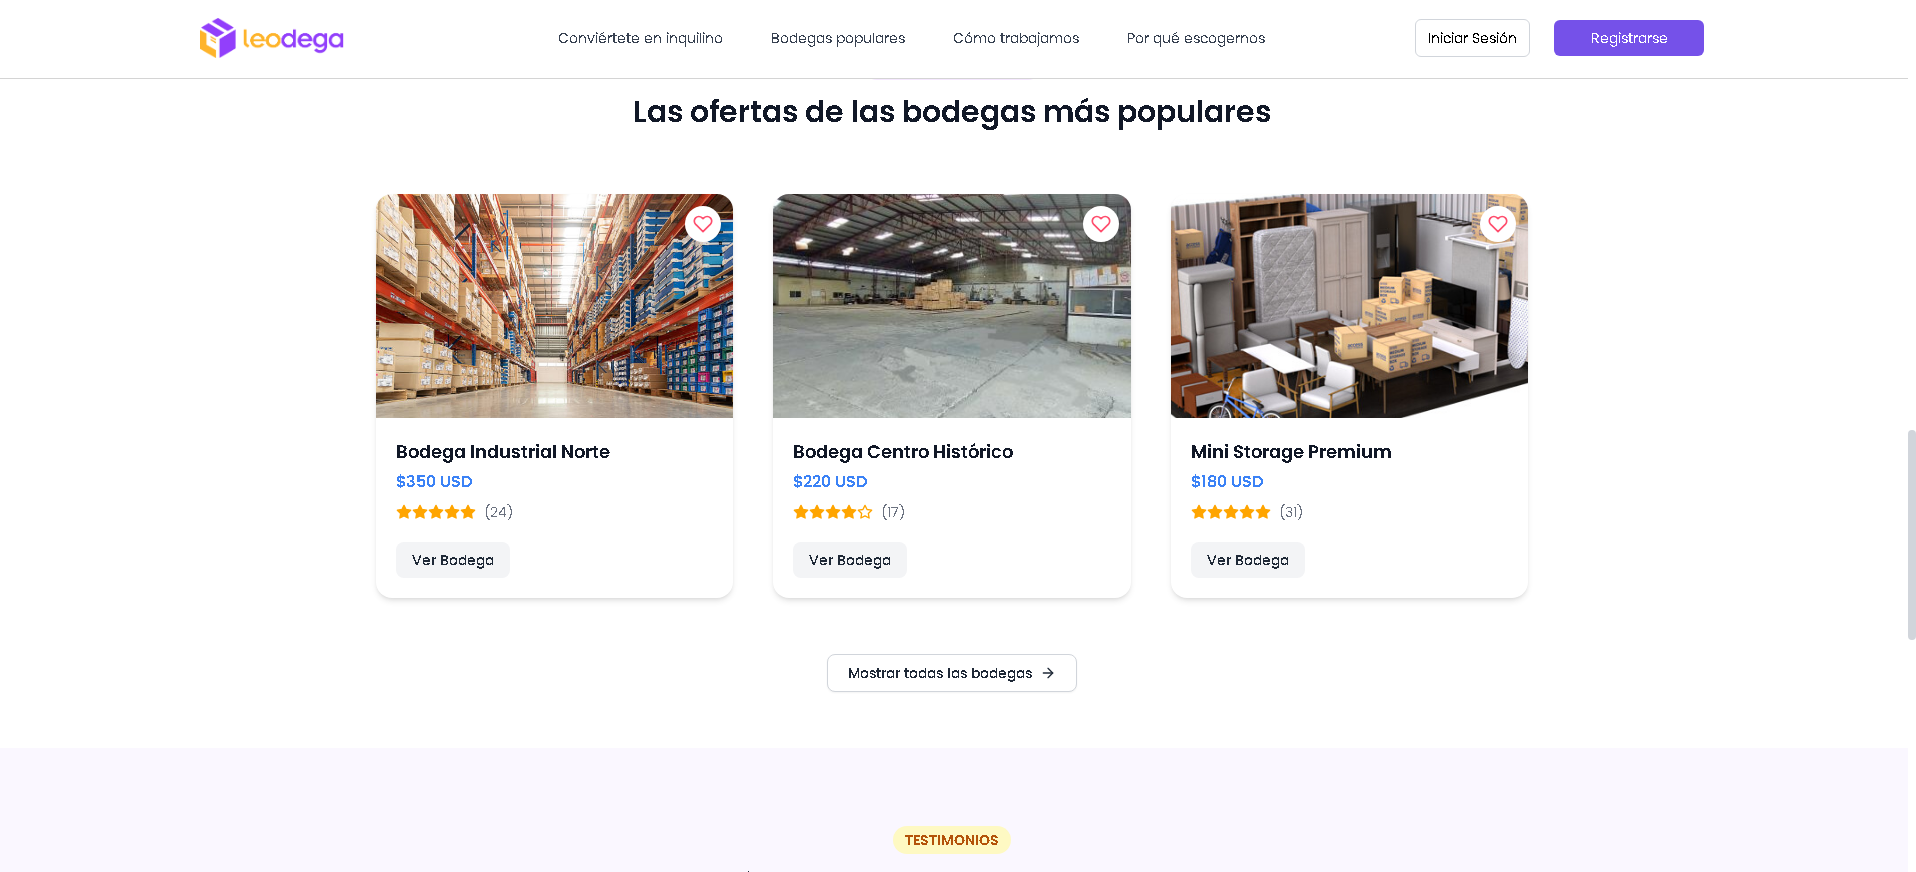
\includegraphics[width=\linewidth]{img/fig04_popular_warehouses}
    \caption{Landing Page: ``Popular Warehouses'' section showing
    featured listings with price and rating.}
    \label{fig:popular_warehouses}
\end{figure}

\subsection{Authentication}

The authentication flow allows users to create a new account or sign
in using their own credentials or through third-party providers
(Facebook, Google, Apple).

\begin{figure}[H]
    \centering
    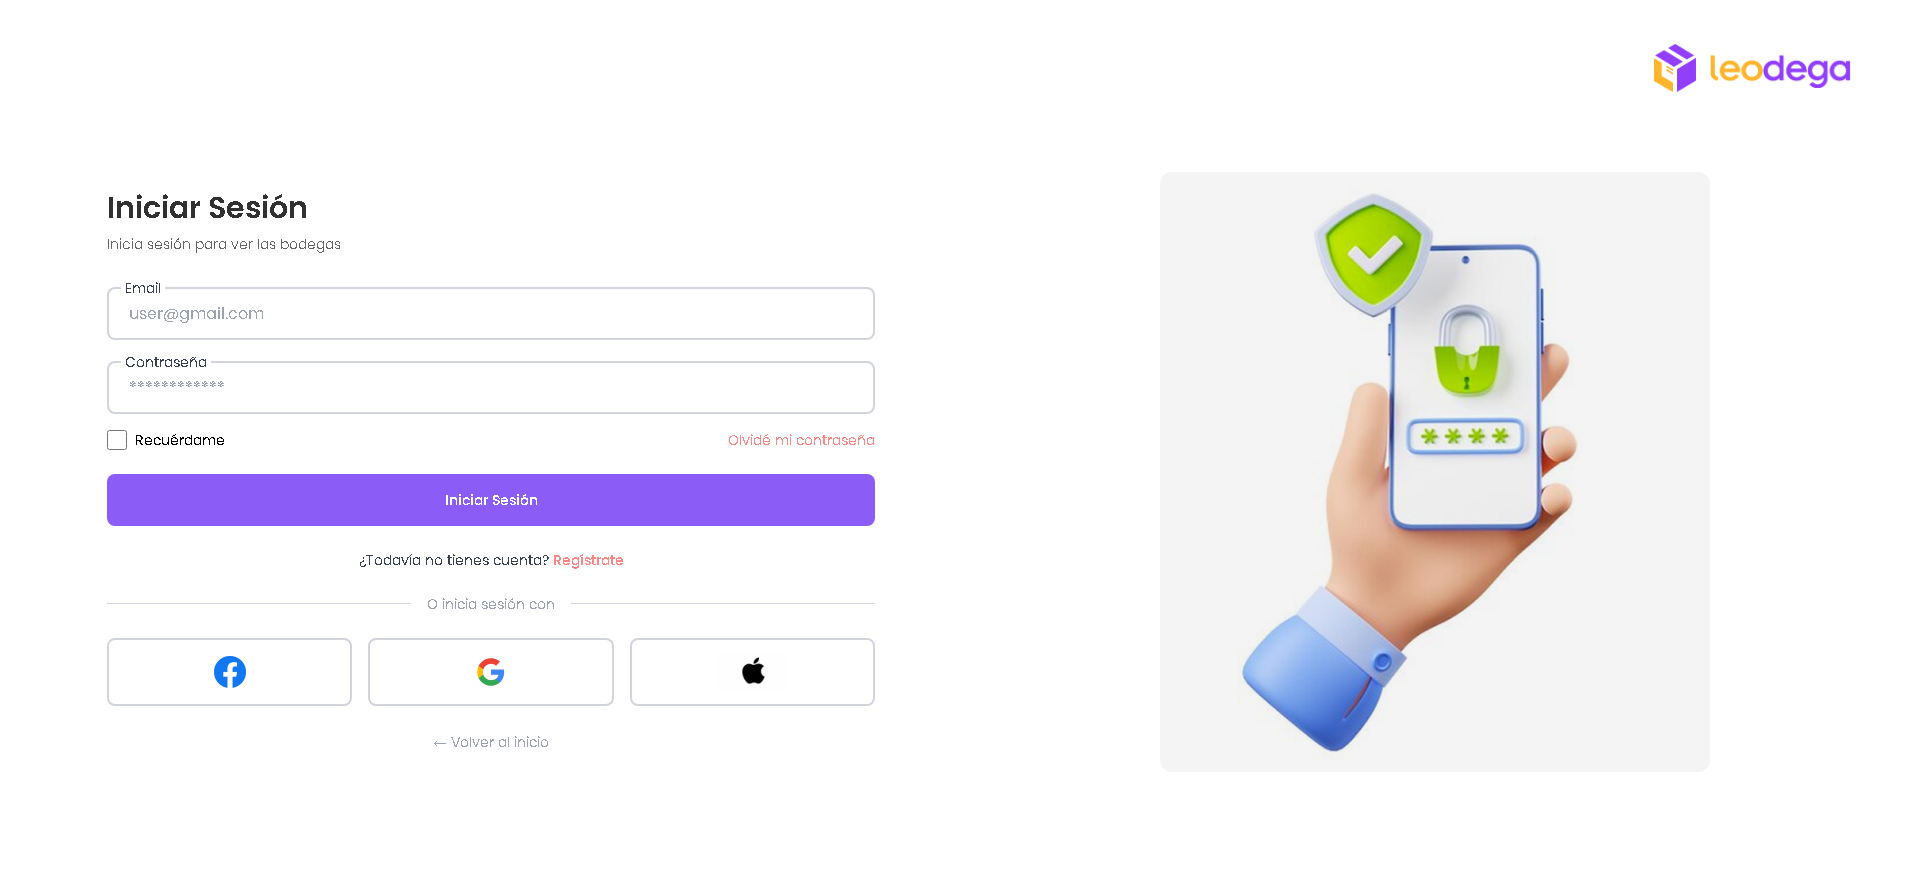
\includegraphics[width=0.85\linewidth]{img/fig05_login}
    \caption{Login screen with email and password form and social
    login options.}
    \label{fig:login}
\end{figure}

\begin{figure}[H]
    \centering
    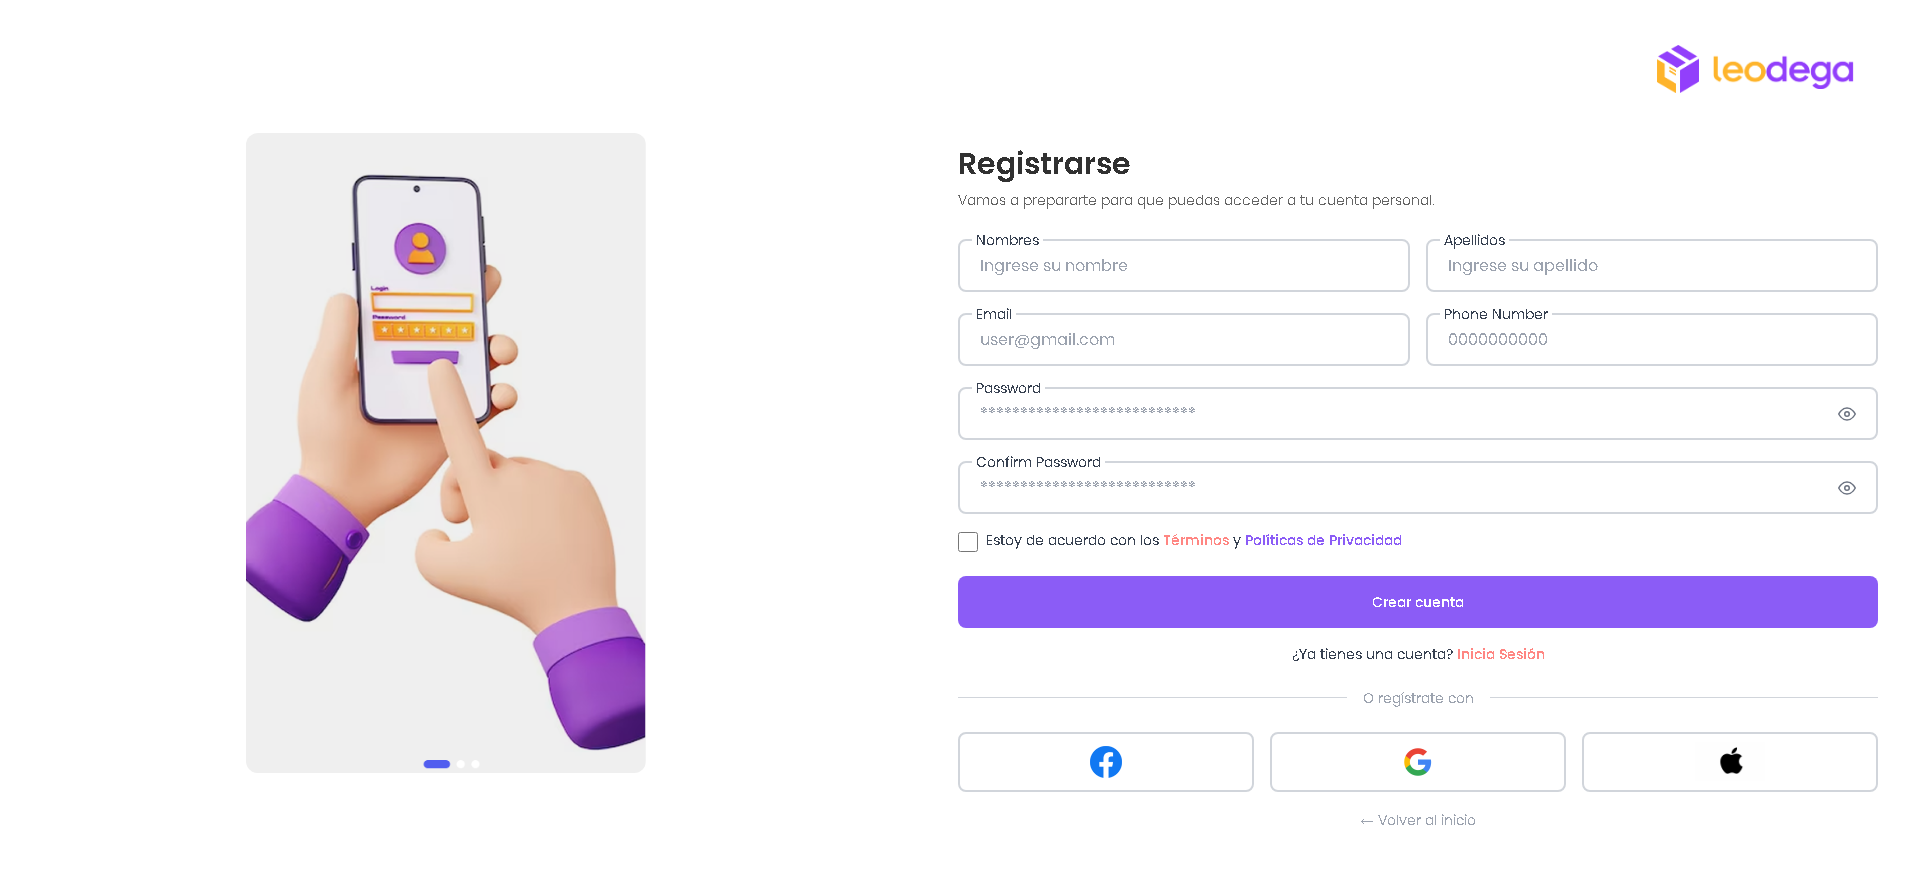
\includegraphics[width=0.85\linewidth]{img/fig06_registration}
    \caption{Registration screen: account creation form with personal
    data and password confirmation.}
    \label{fig:registration}
\end{figure}

\begin{figure}[H]
    \centering
    
\includegraphics[width=0.6\linewidth]{img/fig07_profile_selection}
    \caption{User profile selection: Tenant, Landlord/Manager, or
    Administrator.}
    \label{fig:profile_selection}
\end{figure}

% ───────────────────────────────────────────────────────────────────
\section{Tenant}
% ───────────────────────────────────────────────────────────────────

The Tenant flow enables users to search and filter available
warehouses, view detailed information, complete the booking and
payment process, and manage their active rentals.

\subsection{Warehouse Catalog}

The catalog displays available warehouses with filters for city,
size, and price. Each card shows the type, location, surface area,
rating, and monthly price.

\begin{figure}[H]
    \centering
    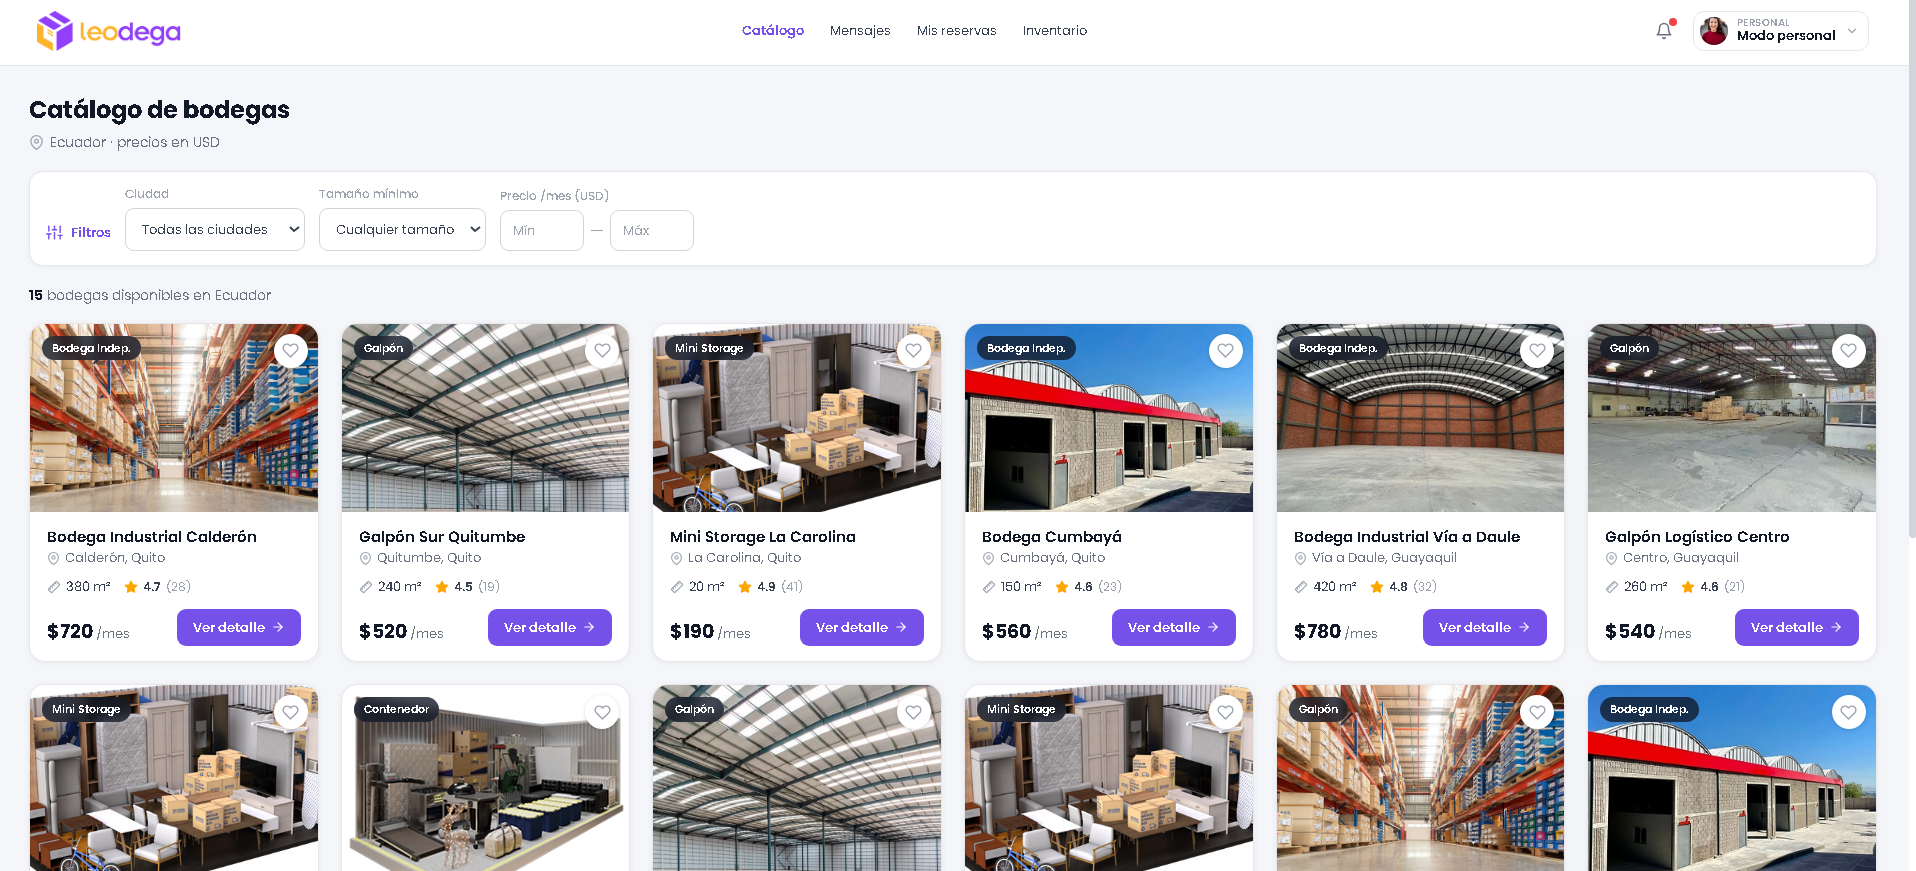
\includegraphics[width=\linewidth]{img/fig08_catalog}
    \caption{Warehouse Catalog: grid view with city, size, and price
    filters (15 listings shown).}
    \label{fig:catalog}
\end{figure}

\subsection{Warehouse Detail}

The detail view presents a photo gallery, full description, features,
assigned manager, availability calendar, location map, and cost
breakdown.

\begin{figure}[H]
    \centering
    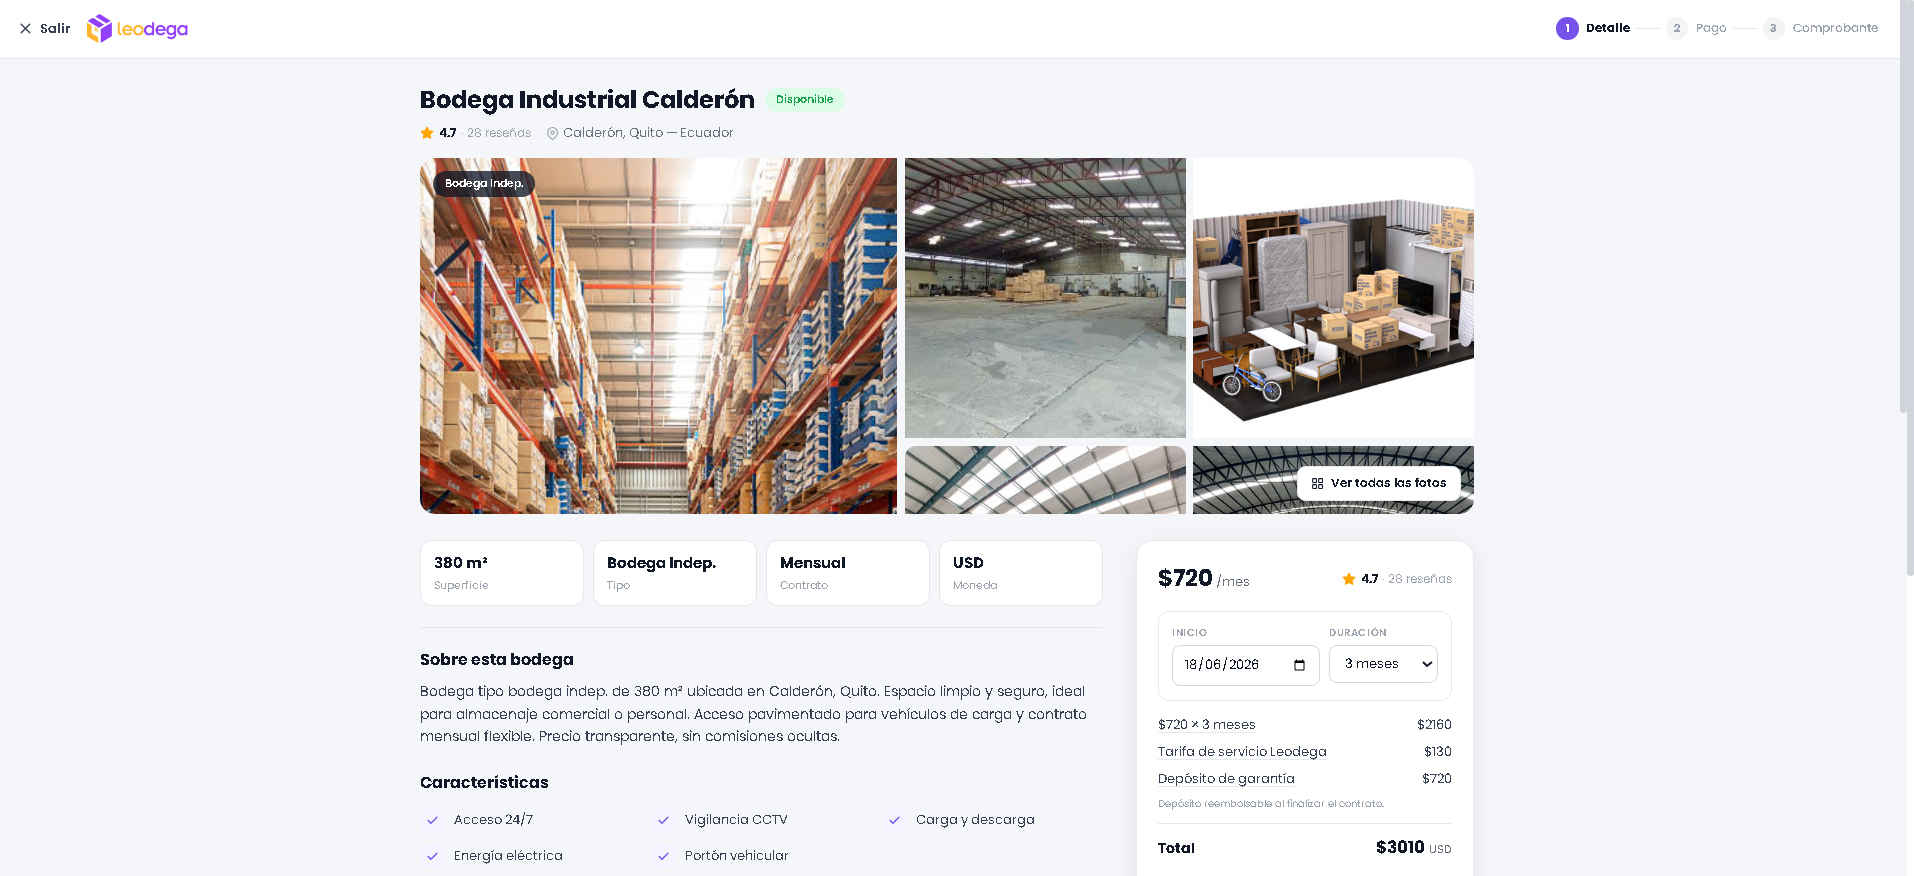
\includegraphics[width=\linewidth]{img/fig09_warehouse_detail}
    \caption{Warehouse Detail: photo gallery, features, and cost
    summary (Step 1 of the booking flow).}
    \label{fig:warehouse_detail}
\end{figure}

\begin{figure}[H]
    \centering
    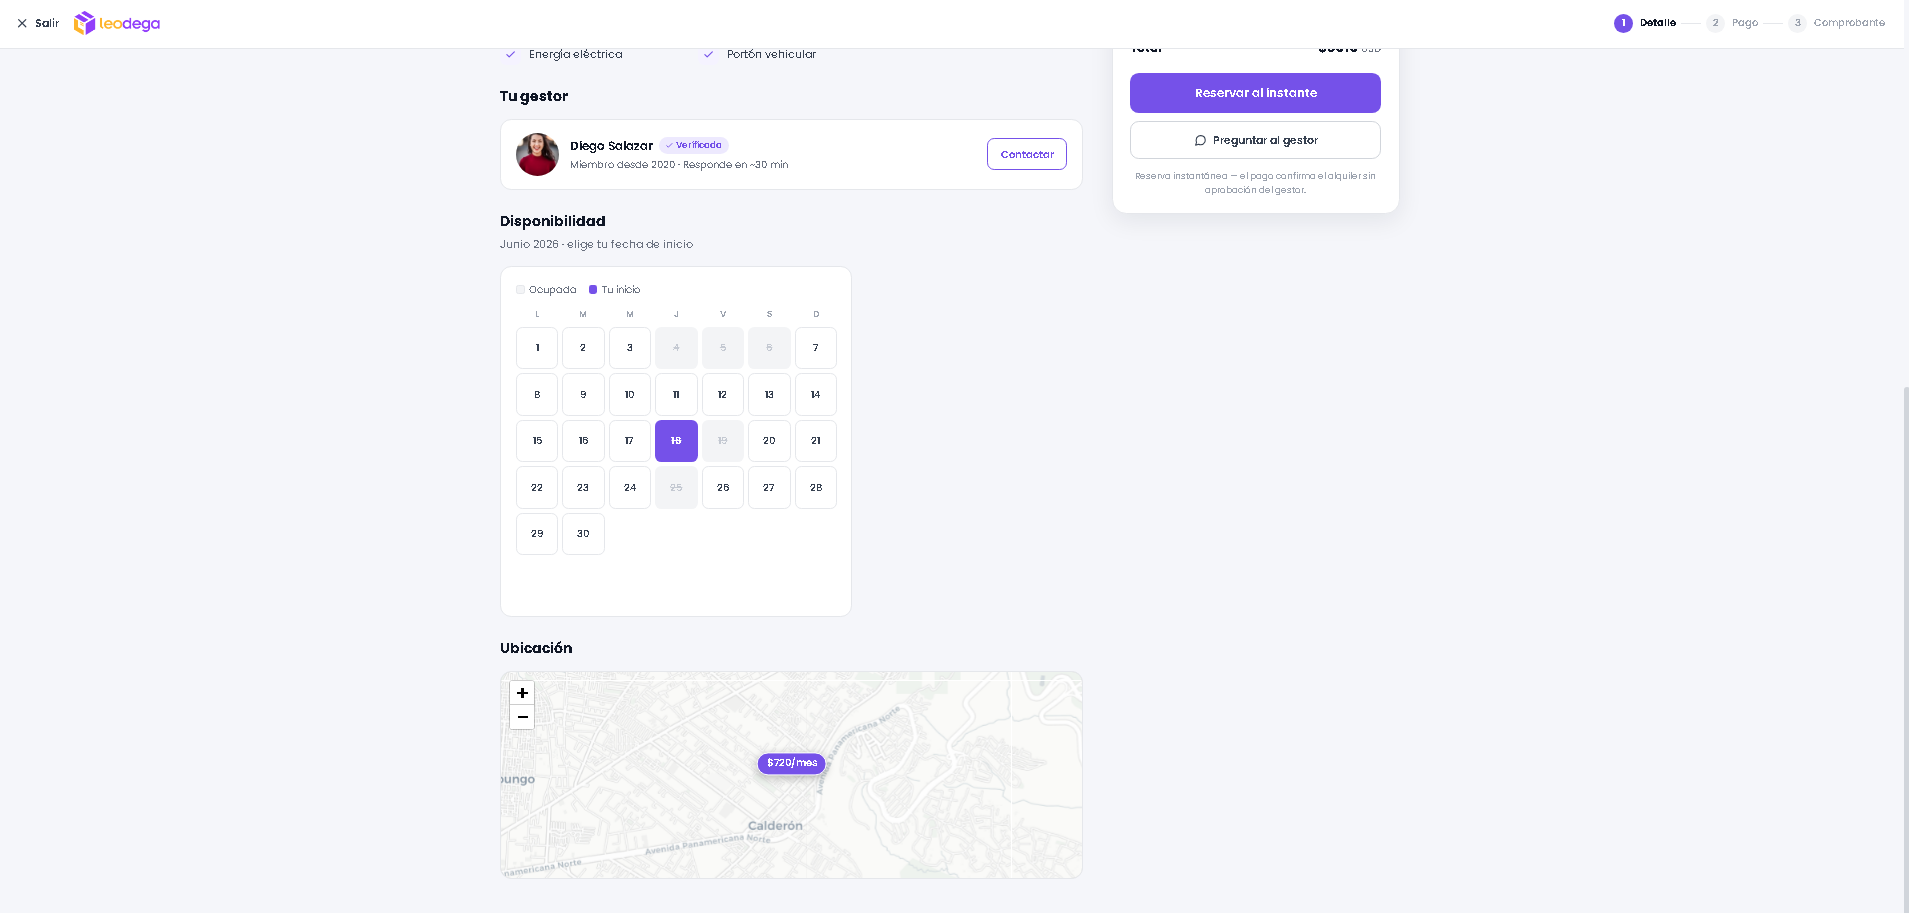
\includegraphics[width=\linewidth]{img/fig10_warehouse_calendar}
    \caption{Warehouse Detail: manager information, availability
    calendar, and location map.}
    \label{fig:warehouse_calendar}
\end{figure}

\subsection{Booking and Payment Process}

The booking flow consists of three steps: Detail, Payment, and
Receipt. The payment step collects card information and shows the
final cost breakdown before confirmation.

\begin{figure}[H]
    \centering
    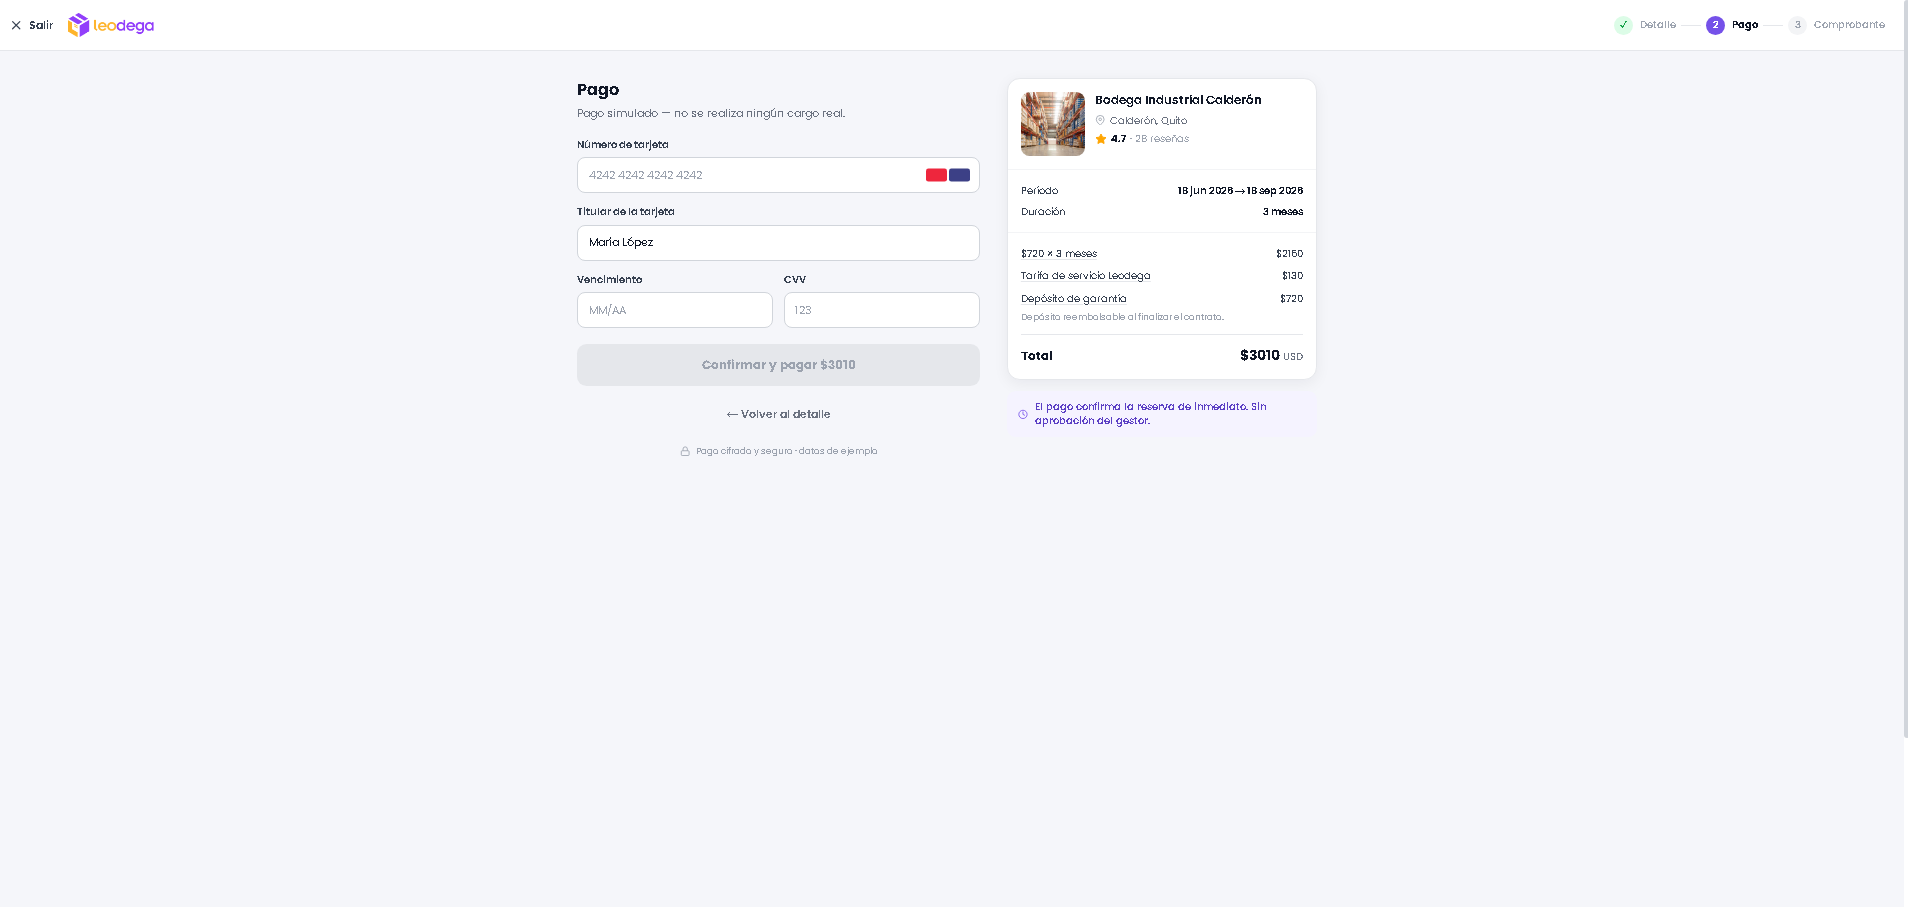
\includegraphics[width=\linewidth]{img/fig11_payment}
    \caption{Step 2 -- Payment: card details form and total cost
    summary (\$3,010 USD).}
    \label{fig:payment}
\end{figure}

\subsection{My Bookings}

The bookings panel groups rentals into Active, Completed, and
Cancelled tabs, with options to cancel or report an issue.

\begin{figure}[H]
    \centering
    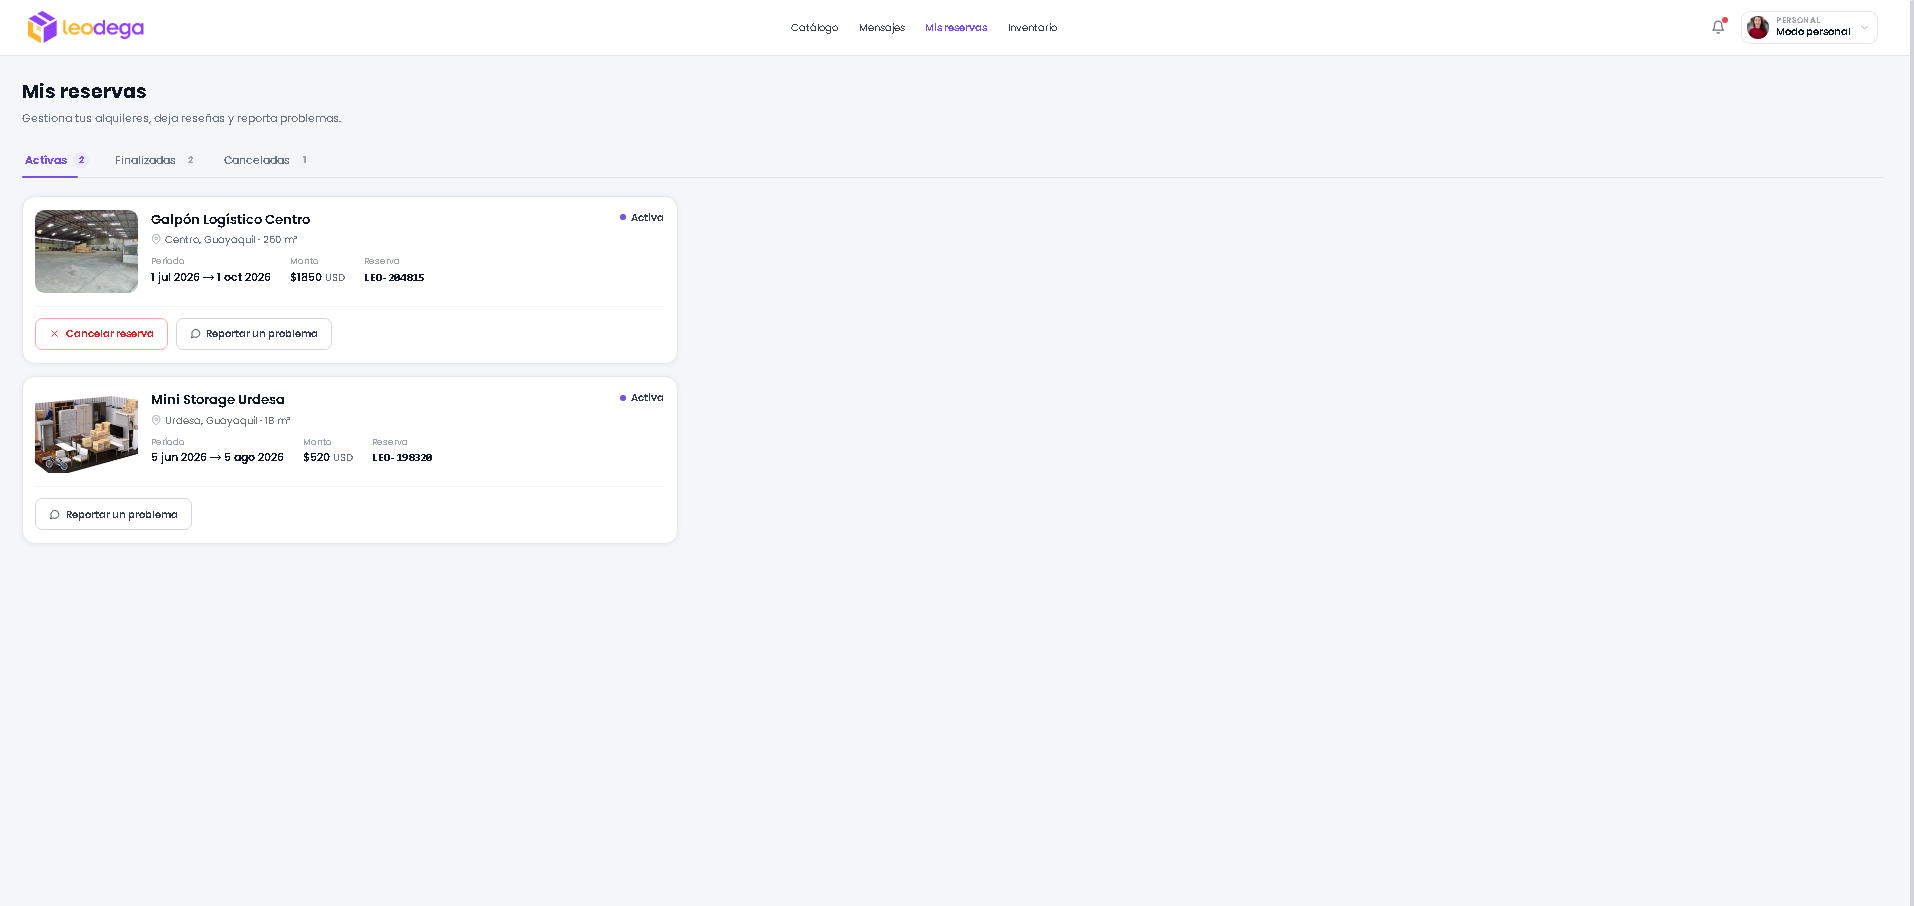
\includegraphics[width=\linewidth]{img/fig12_my_bookings}
    \caption{My Bookings: active rentals list with period, amount,
    and booking reference code.}
    \label{fig:my_bookings}
\end{figure}

\subsection{Messages}

The messaging module allows tenants to communicate with warehouse
managers for pre-booking inquiries and during active rental periods.

\begin{figure}[H]
    \centering
    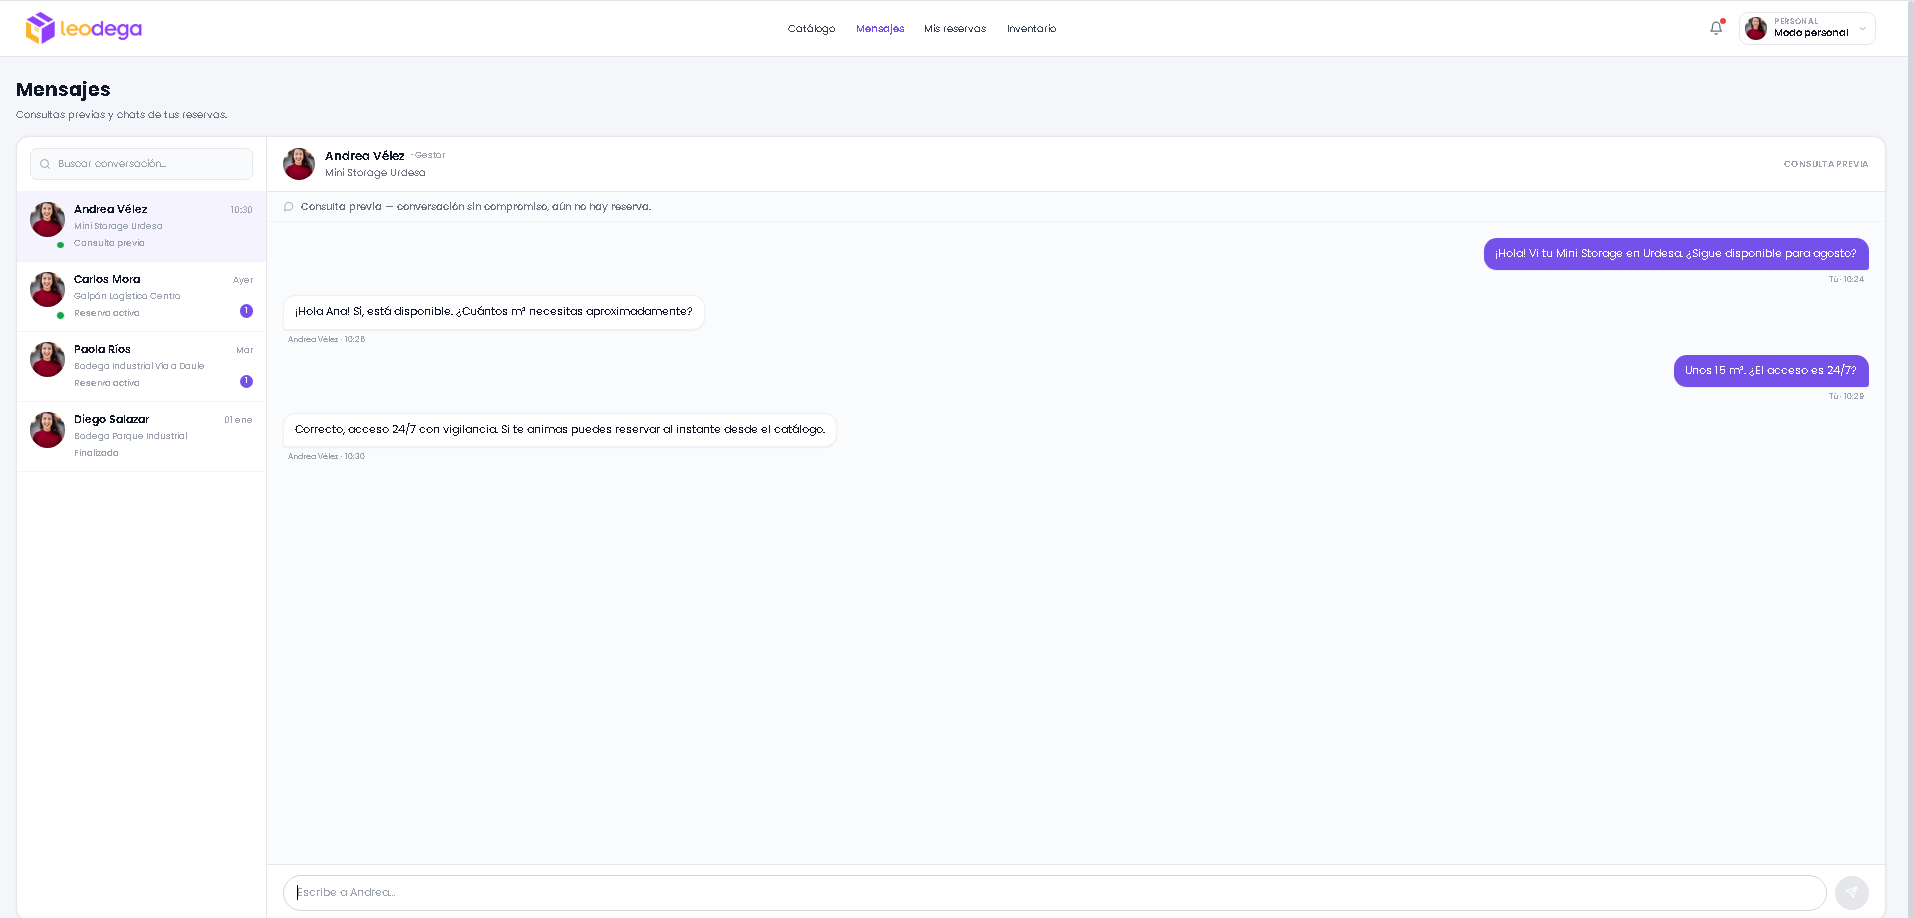
\includegraphics[width=\linewidth]{img/fig13_tenant_messages}
    \caption{Tenant Messages: inbox with per-warehouse conversations
    and real-time chat with the manager.}
    \label{fig:tenant_messages}
\end{figure}

\subsection{Inventory}

The inventory module allows tenants to connect an external system via
a read-only endpoint URL to display stock data directly within
Leodega.

\begin{figure}[H]
    \centering
    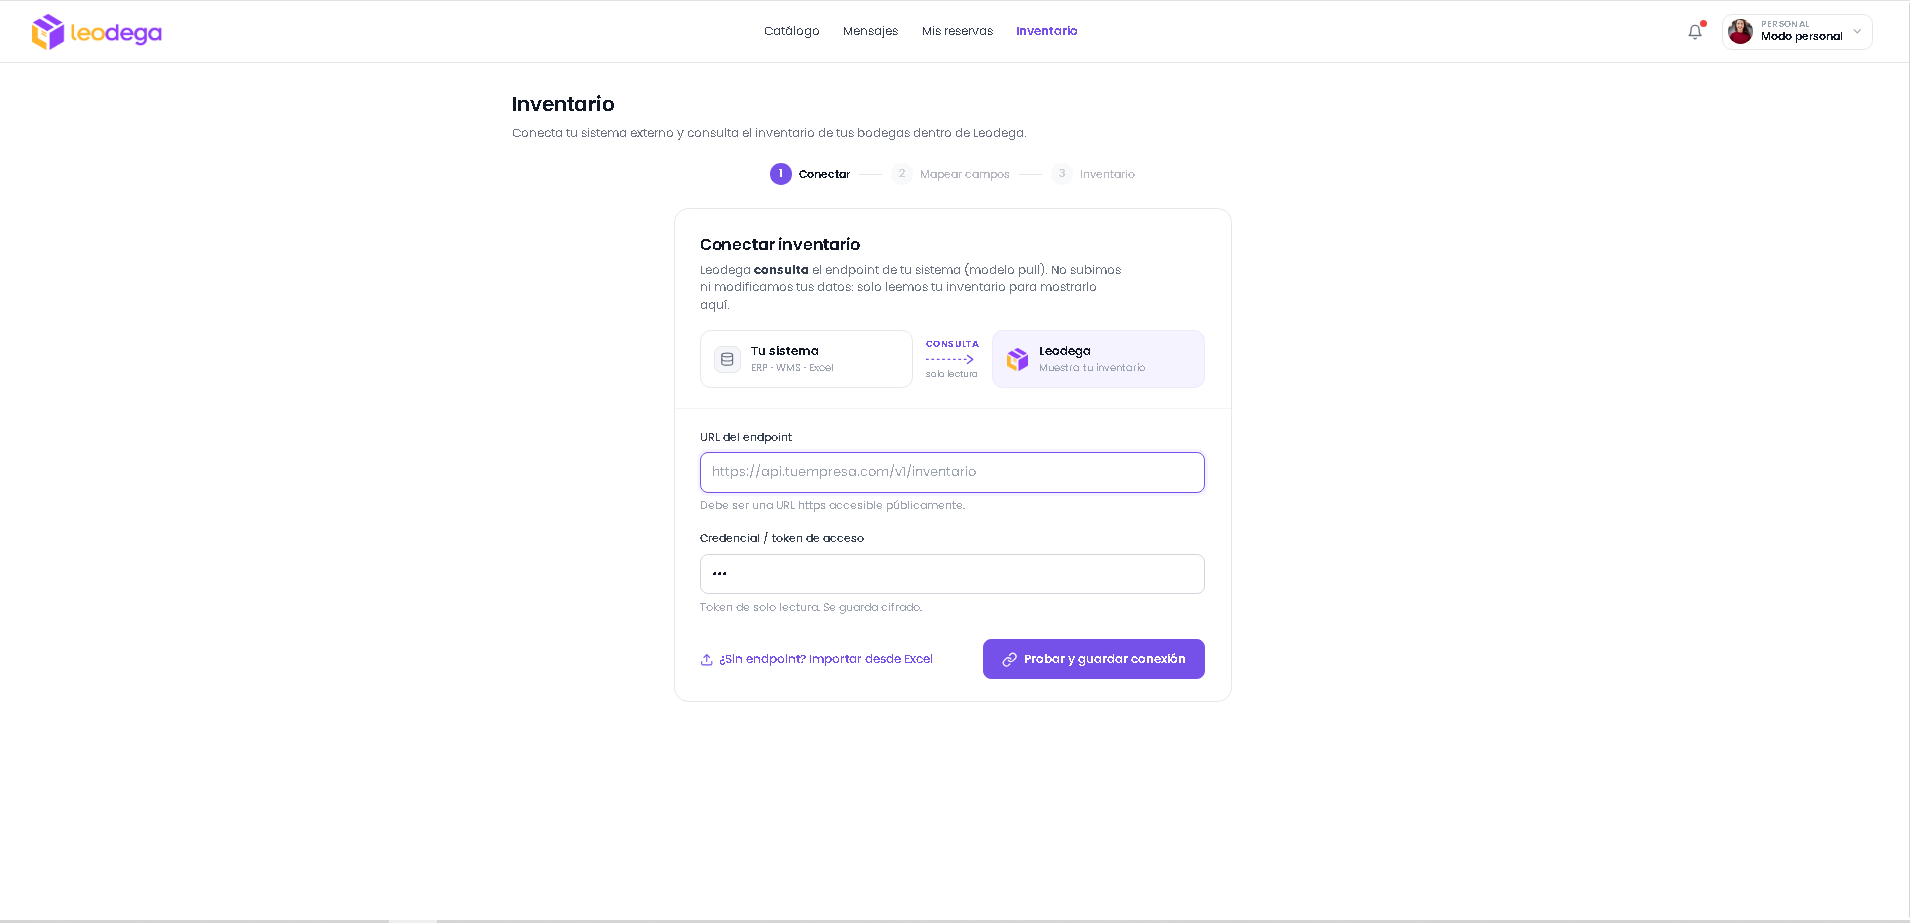
\includegraphics[width=\linewidth]{img/fig14_inventory}
    \caption{Inventory: external system connection via endpoint URL
    and read-only access token.}
    \label{fig:inventory}
\end{figure}

% ───────────────────────────────────────────────────────────────────
\section{Landlord / Manager}
% ───────────────────────────────────────────────────────────────────

The Landlord/Manager role provides a management panel for publishing
warehouses, tracking incoming bookings, communicating with tenants,
and monitoring the occupancy calendar.

\subsection{Main Panel: My Warehouses}

The central view lists all published warehouses filtered by
verification status: Approved, Pending, Occupied, Rejected, and
Inactive.

\begin{figure}[H]
    \centering
    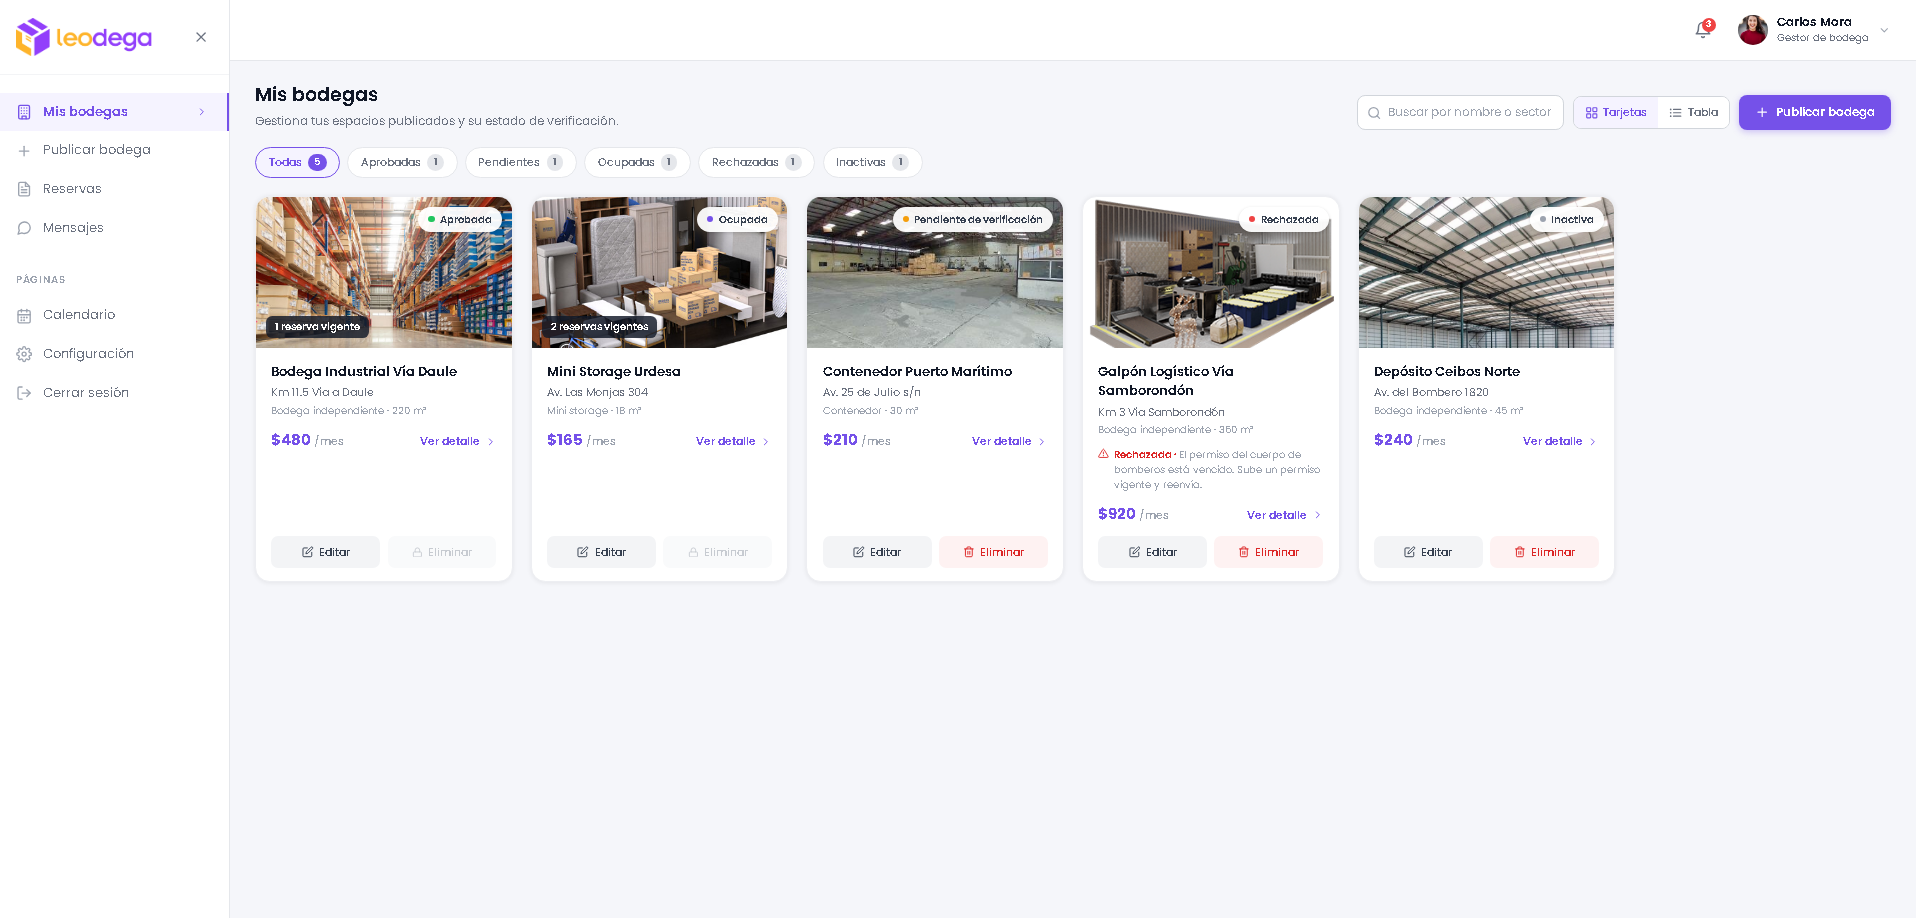
\includegraphics[width=\linewidth]{img/fig15_my_warehouses_all}
    \caption{My Warehouses: main panel with five warehouses across
    different verification states.}
    \label{fig:my_warehouses_all}
\end{figure}

\begin{figure}[H]
    \centering
    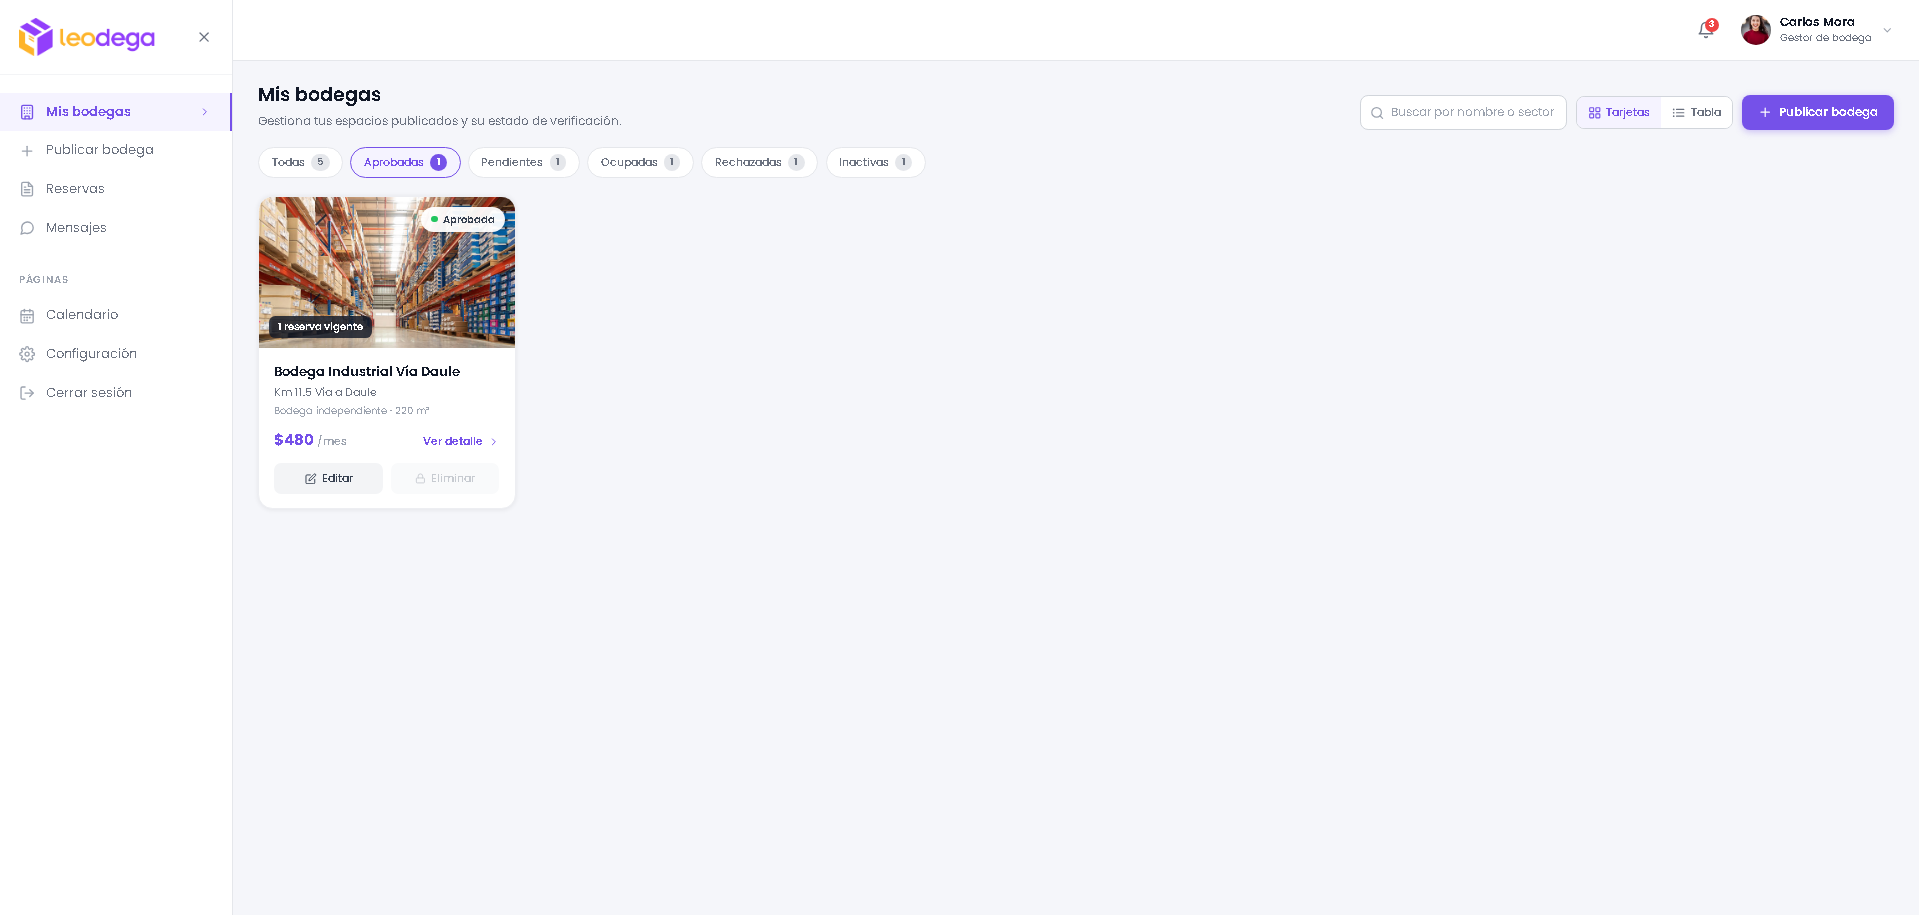
\includegraphics[width=\linewidth]{img/fig16_my_warehouses_approved}
    \caption{My Warehouses: ``Approved'' filter showing an active
    warehouse with one ongoing booking.}
    \label{fig:my_warehouses_approved}
\end{figure}

\subsection{Publish Warehouse}

A guided seven-step flow for listing a new warehouse: space type,
storage modality, photos, location, title and description, pricing
and size, and security documentation.

\begin{figure}[H]
    \centering
    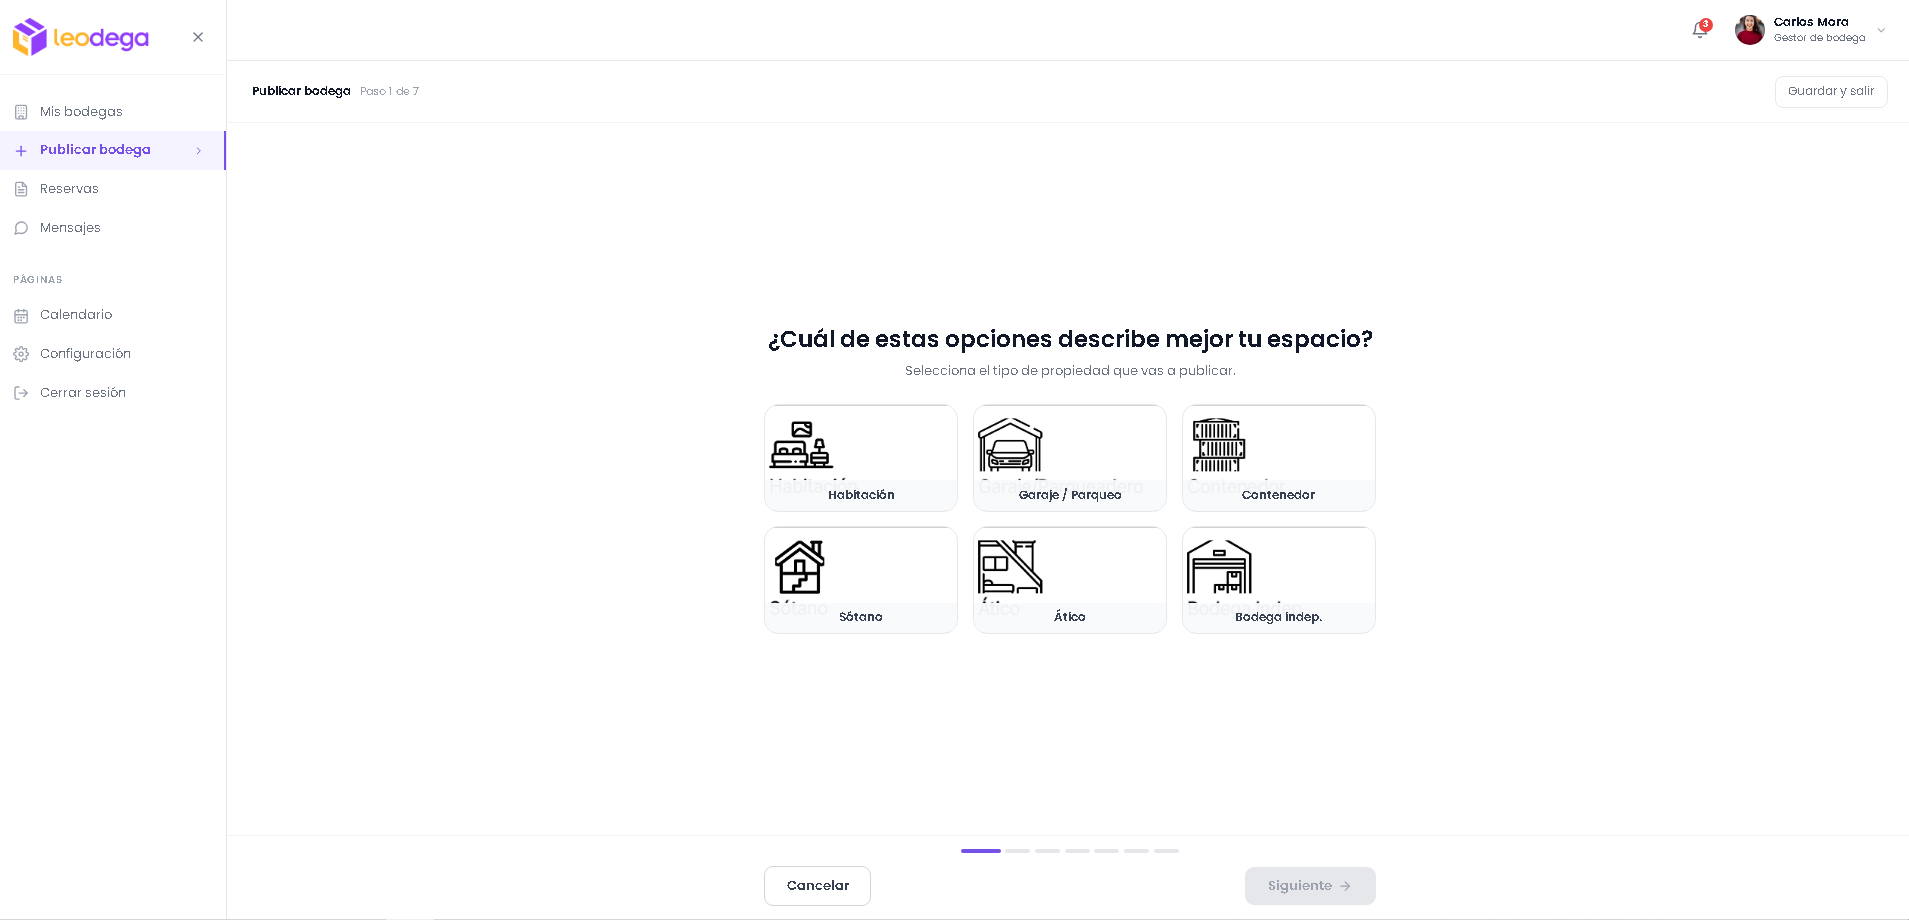
\includegraphics[width=\linewidth]{img/fig17_publish_step1}
    \caption{Publish Warehouse, Step 1/7: space type selection.}
    \label{fig:publish_step1}
\end{figure}

\begin{figure}[H]
    \centering
    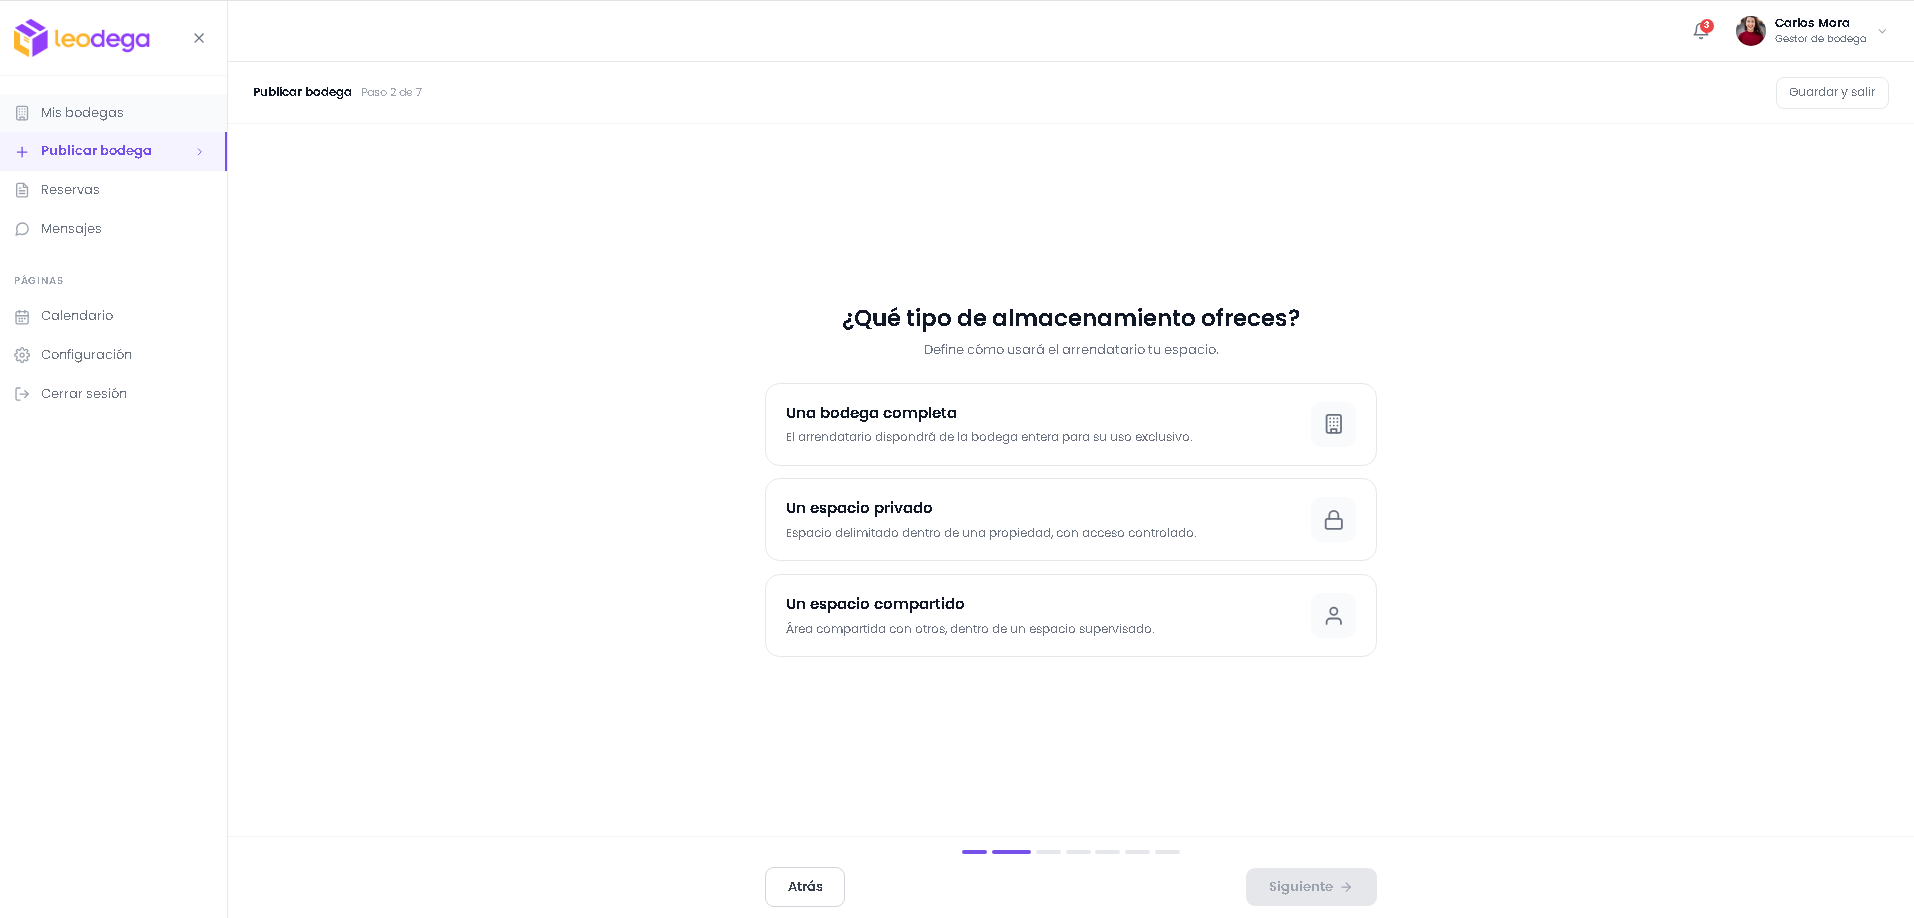
\includegraphics[width=\linewidth]{img/fig18_publish_step2}
    \caption{Publish Warehouse, Step 2/7: storage modality
    (complete, private, or shared).}
    \label{fig:publish_step2}
\end{figure}

\begin{figure}[H]
    \centering
    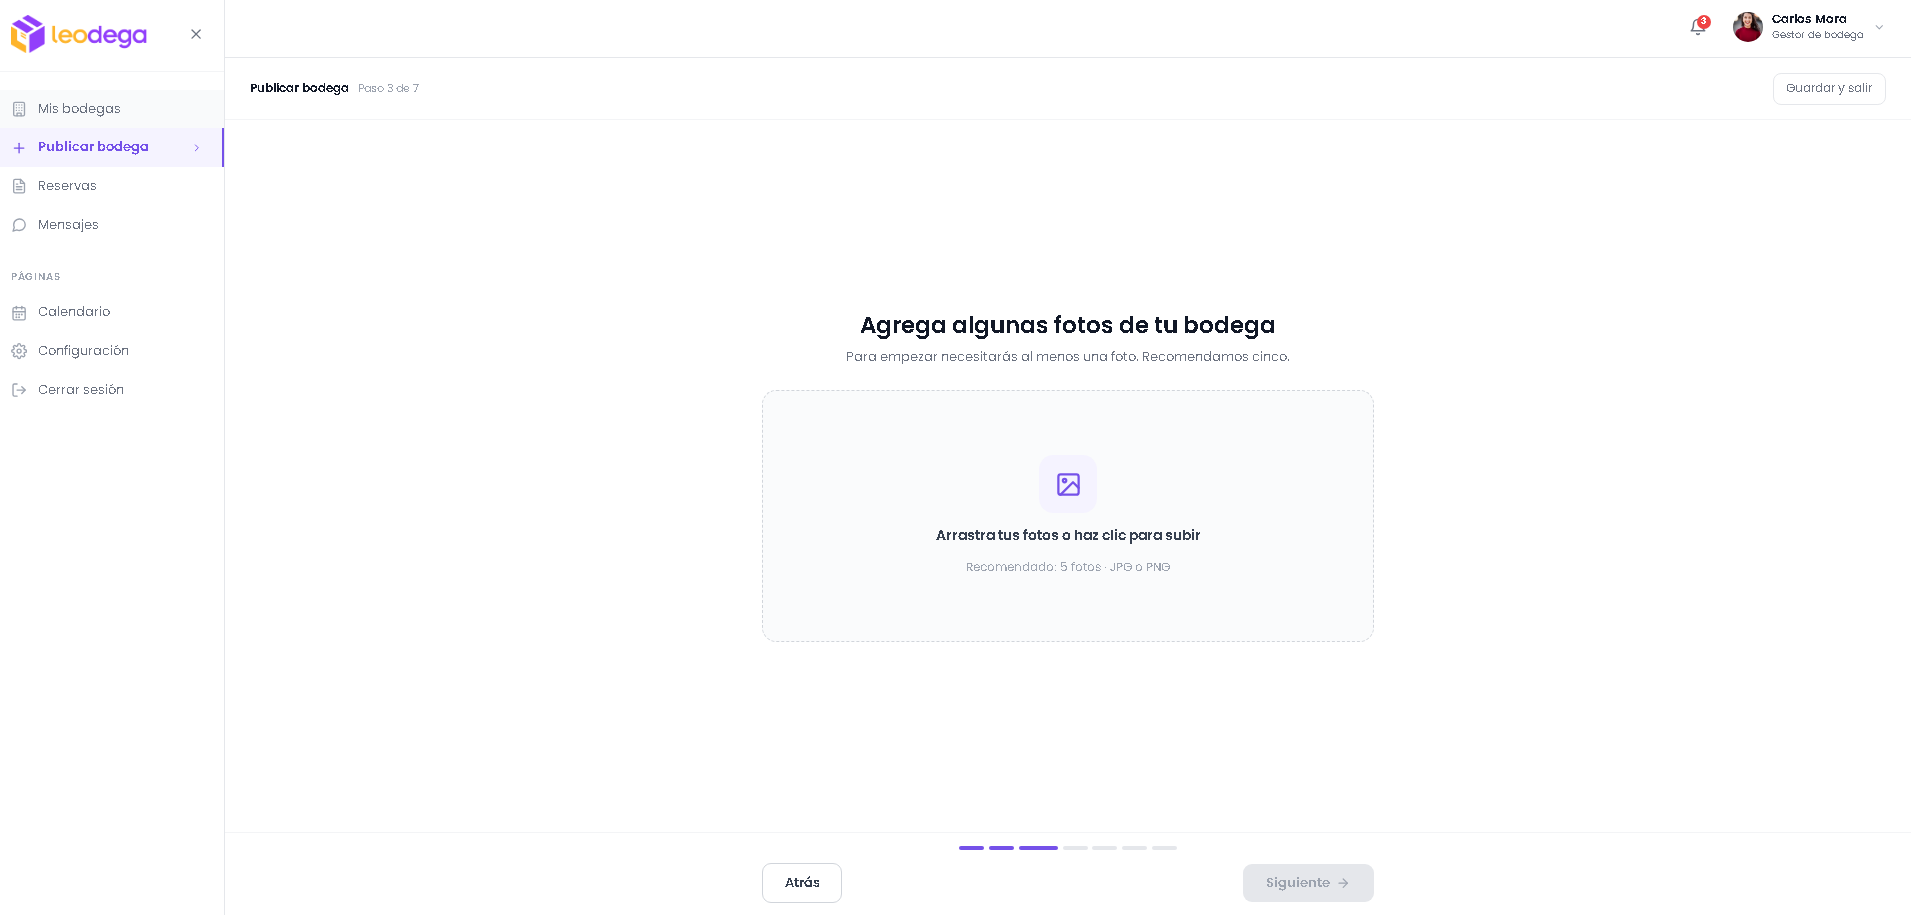
\includegraphics[width=\linewidth]{img/fig19_publish_step3}
    \caption{Publish Warehouse, Step 3/7: photo upload
    (minimum 1, recommended 5).}
    \label{fig:publish_step3}
\end{figure}

\begin{figure}[H]
    \centering
    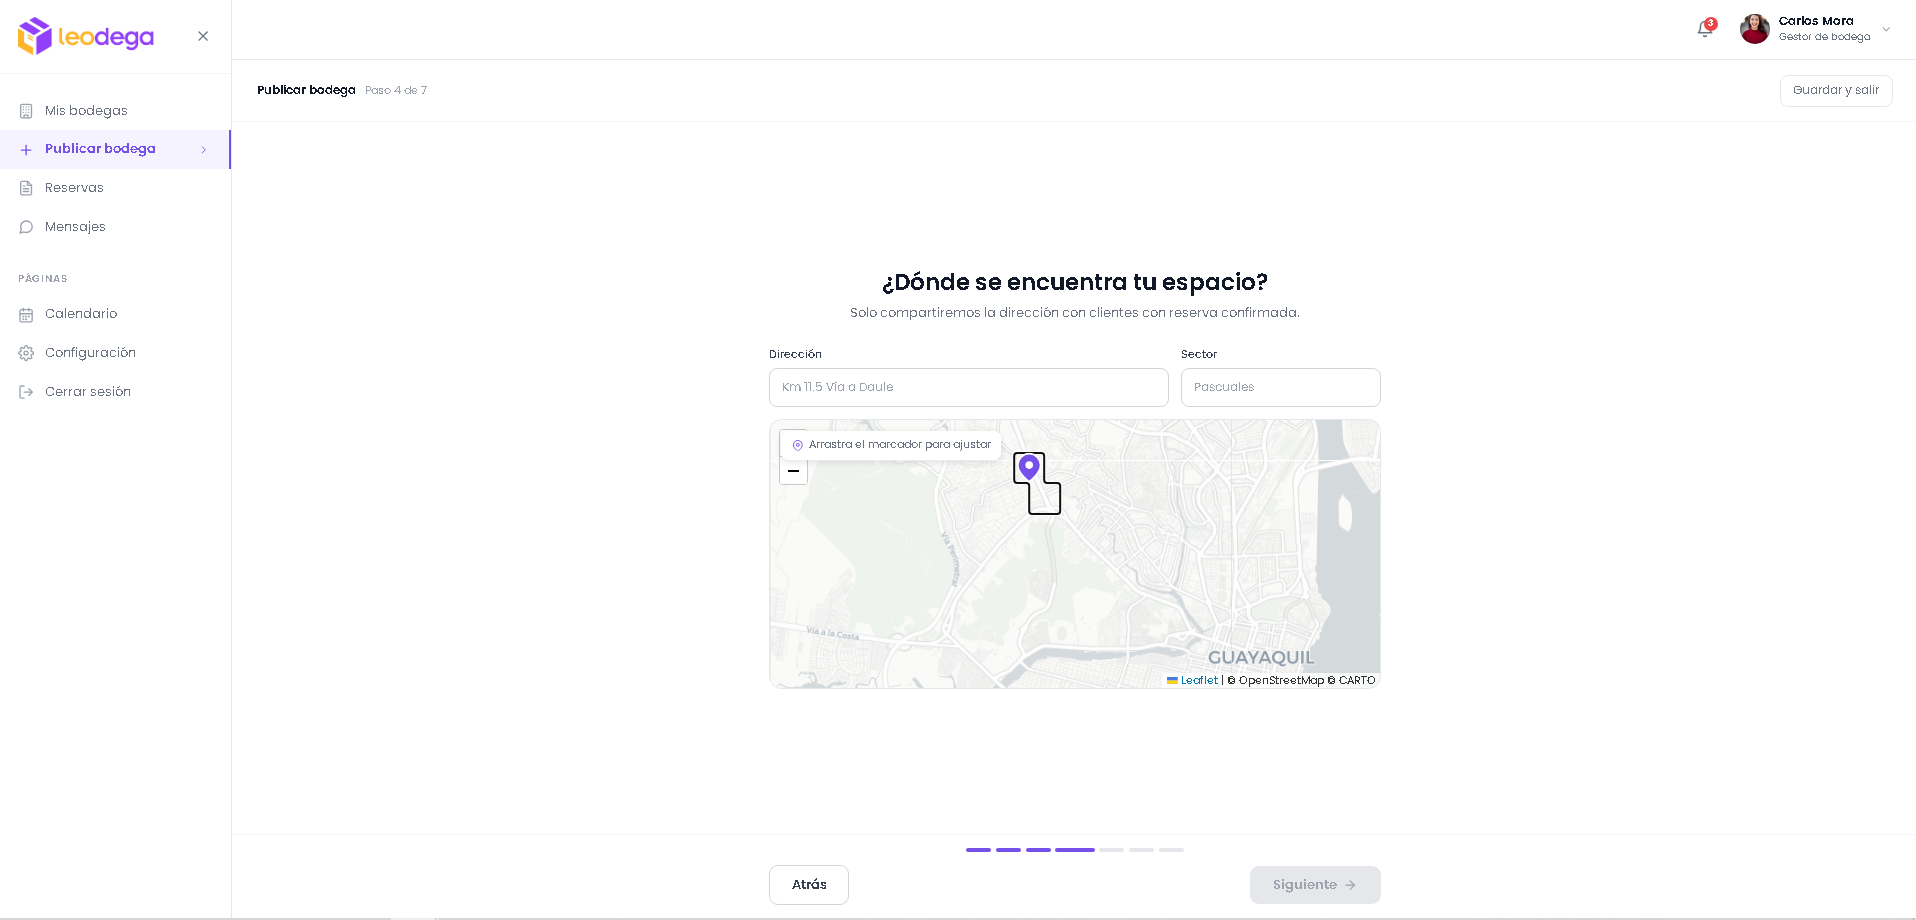
\includegraphics[width=\linewidth]{img/fig20_publish_step4}
    \caption{Publish Warehouse, Step 4/7: location on map with
    address and district fields.}
    \label{fig:publish_step4}
\end{figure}

\begin{figure}[H]
    \centering
    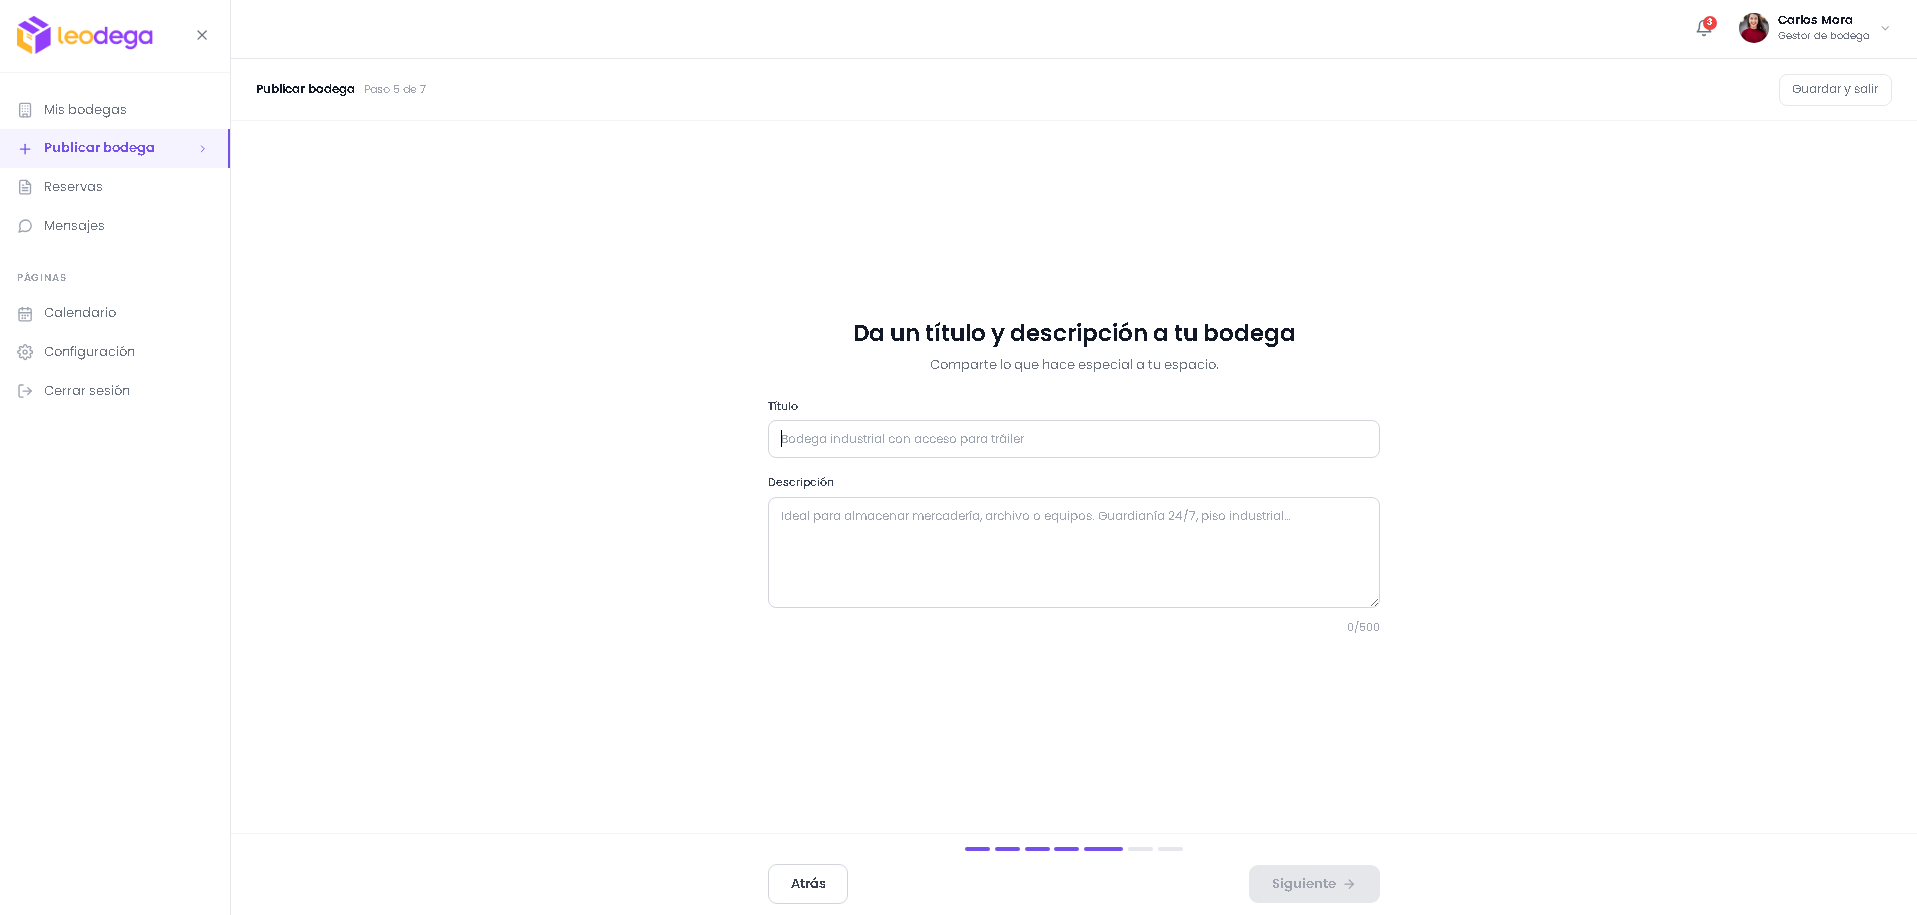
\includegraphics[width=\linewidth]{img/fig21_publish_step5}
    \caption{Publish Warehouse, Step 5/7: title and description
    of the space.}
    \label{fig:publish_step5}
\end{figure}

\begin{figure}[H]
    \centering
    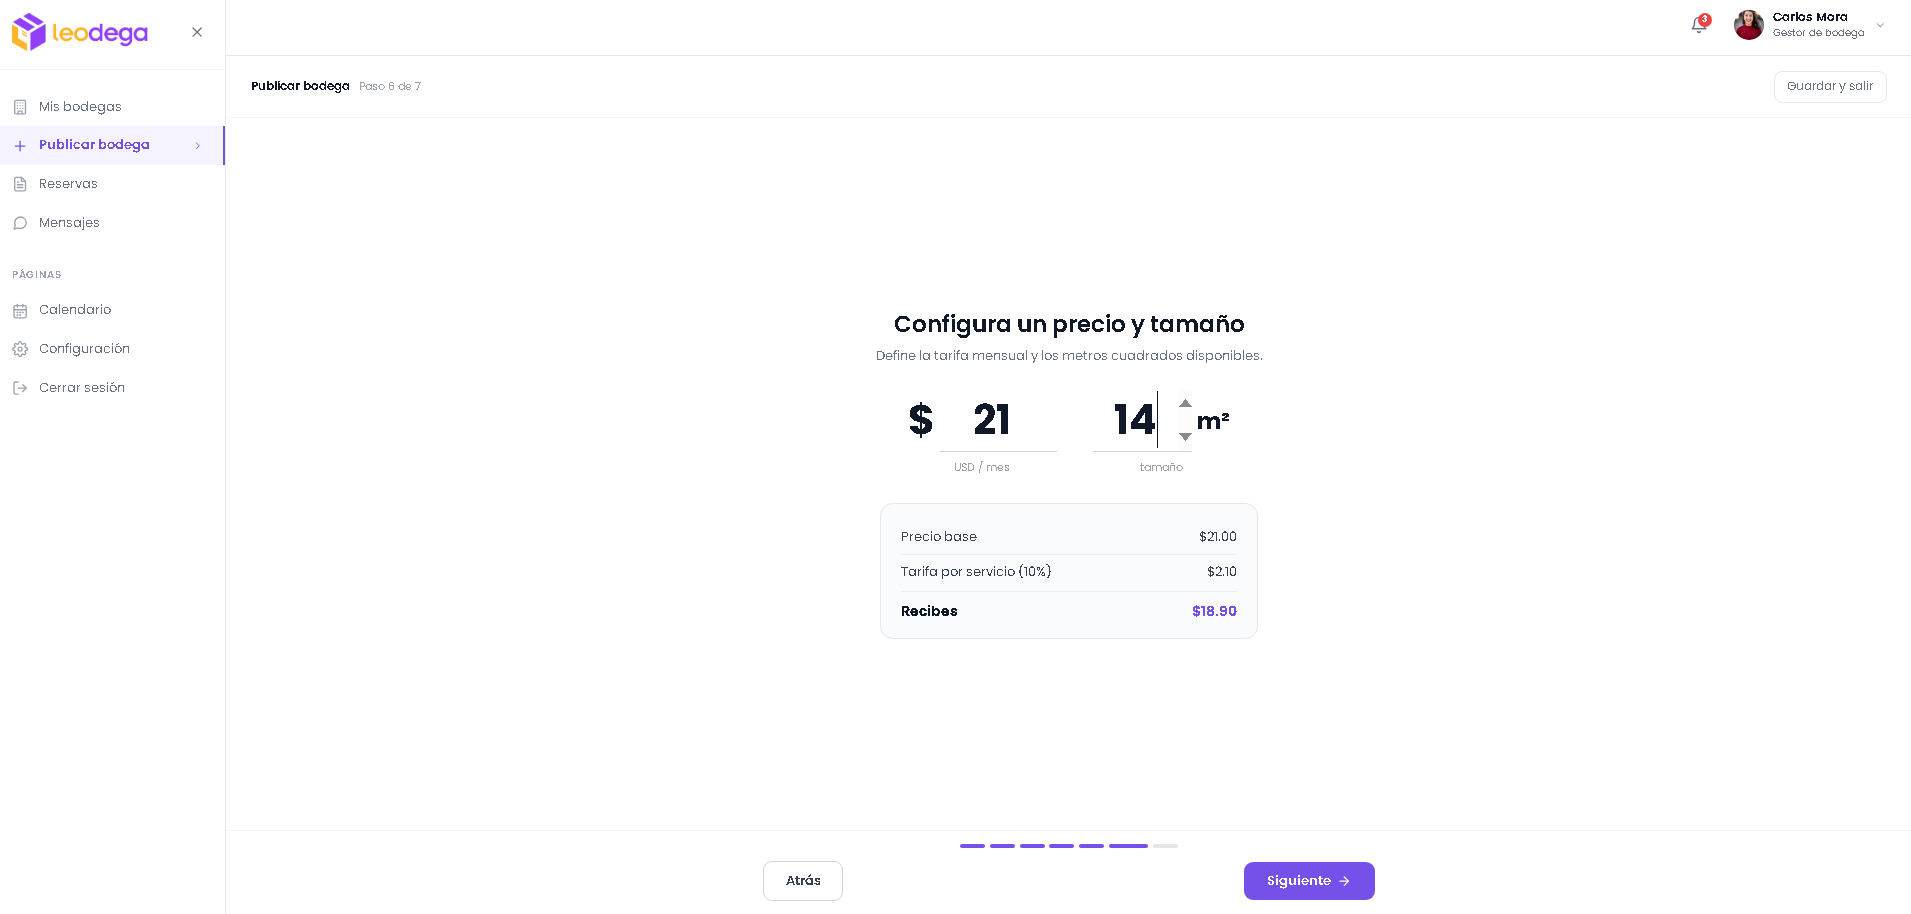
\includegraphics[width=\linewidth]{img/fig22_publish_step6}
    \caption{Publish Warehouse, Step 6/7: monthly price and surface
    area (m$^{2}$) configuration.}
    \label{fig:publish_step6}
\end{figure}

\begin{figure}[H]
    \centering
    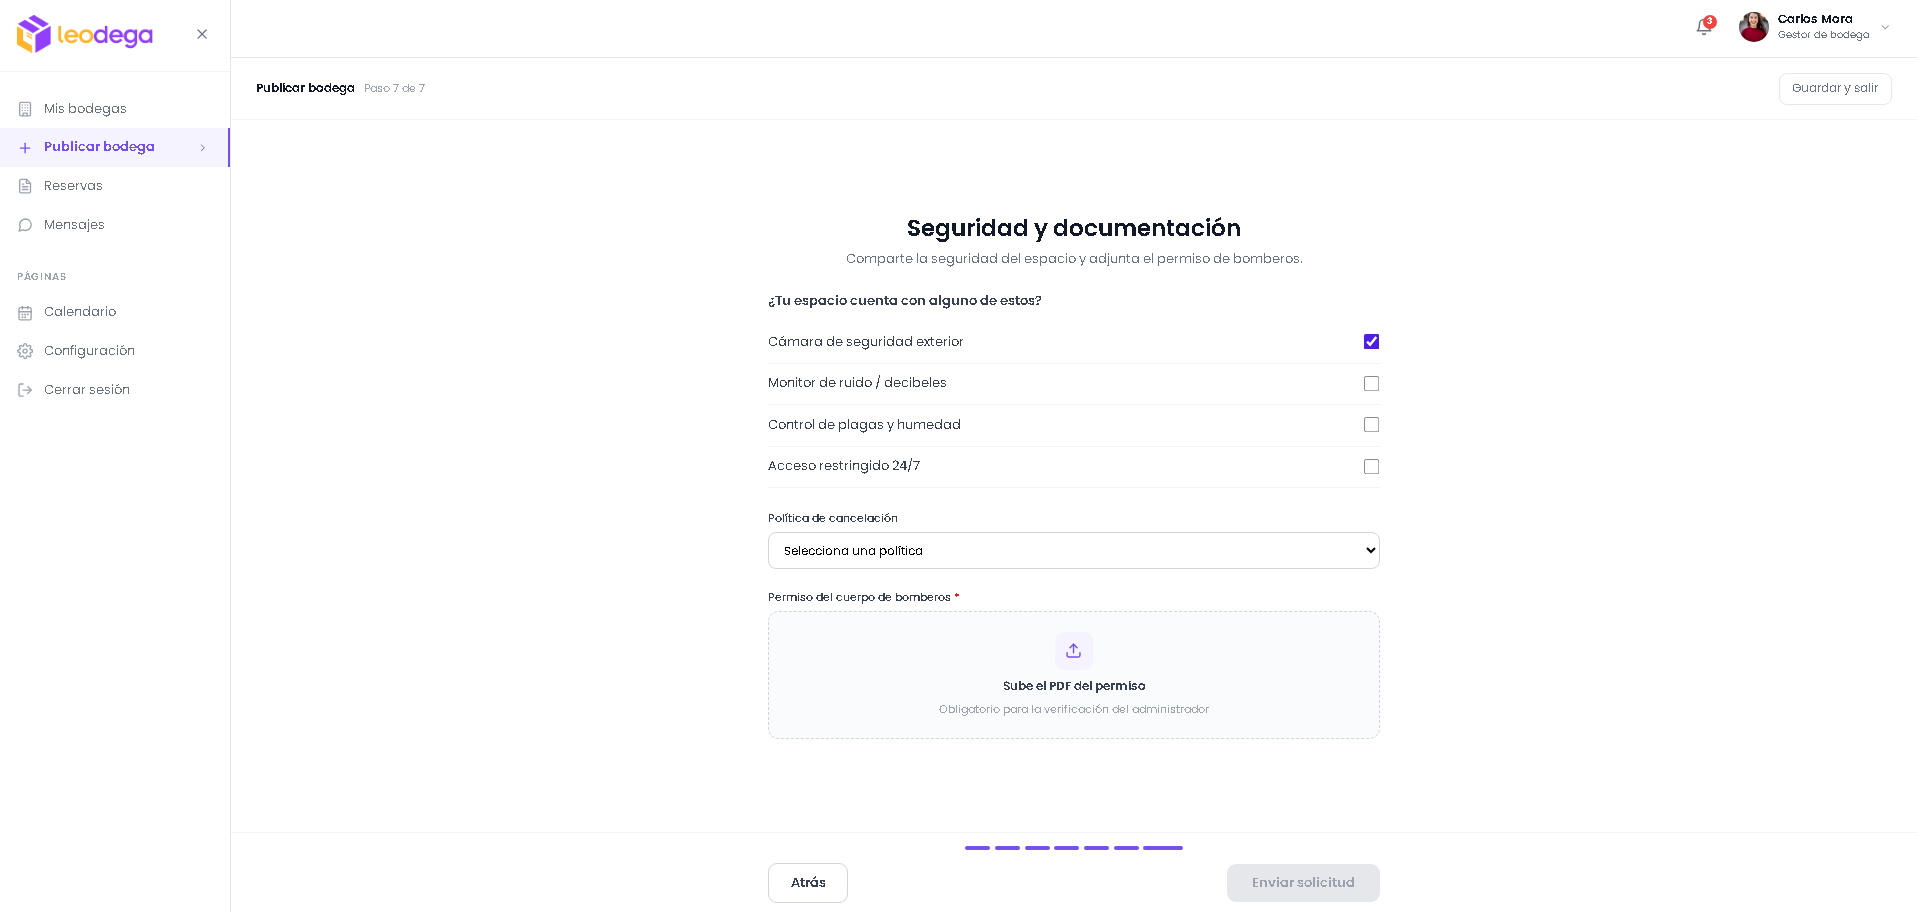
\includegraphics[width=\linewidth]{img/fig23_publish_step7}
    \caption{Publish Warehouse, Step 7/7: security features,
    cancellation policy, and mandatory fire department permit.}
    \label{fig:publish_step7}
\end{figure}

\subsection{Incoming Bookings}

A table view of all bookings across the manager's warehouses with
global metrics and filters by client, payment status, and date range.

\begin{figure}[H]
    \centering
    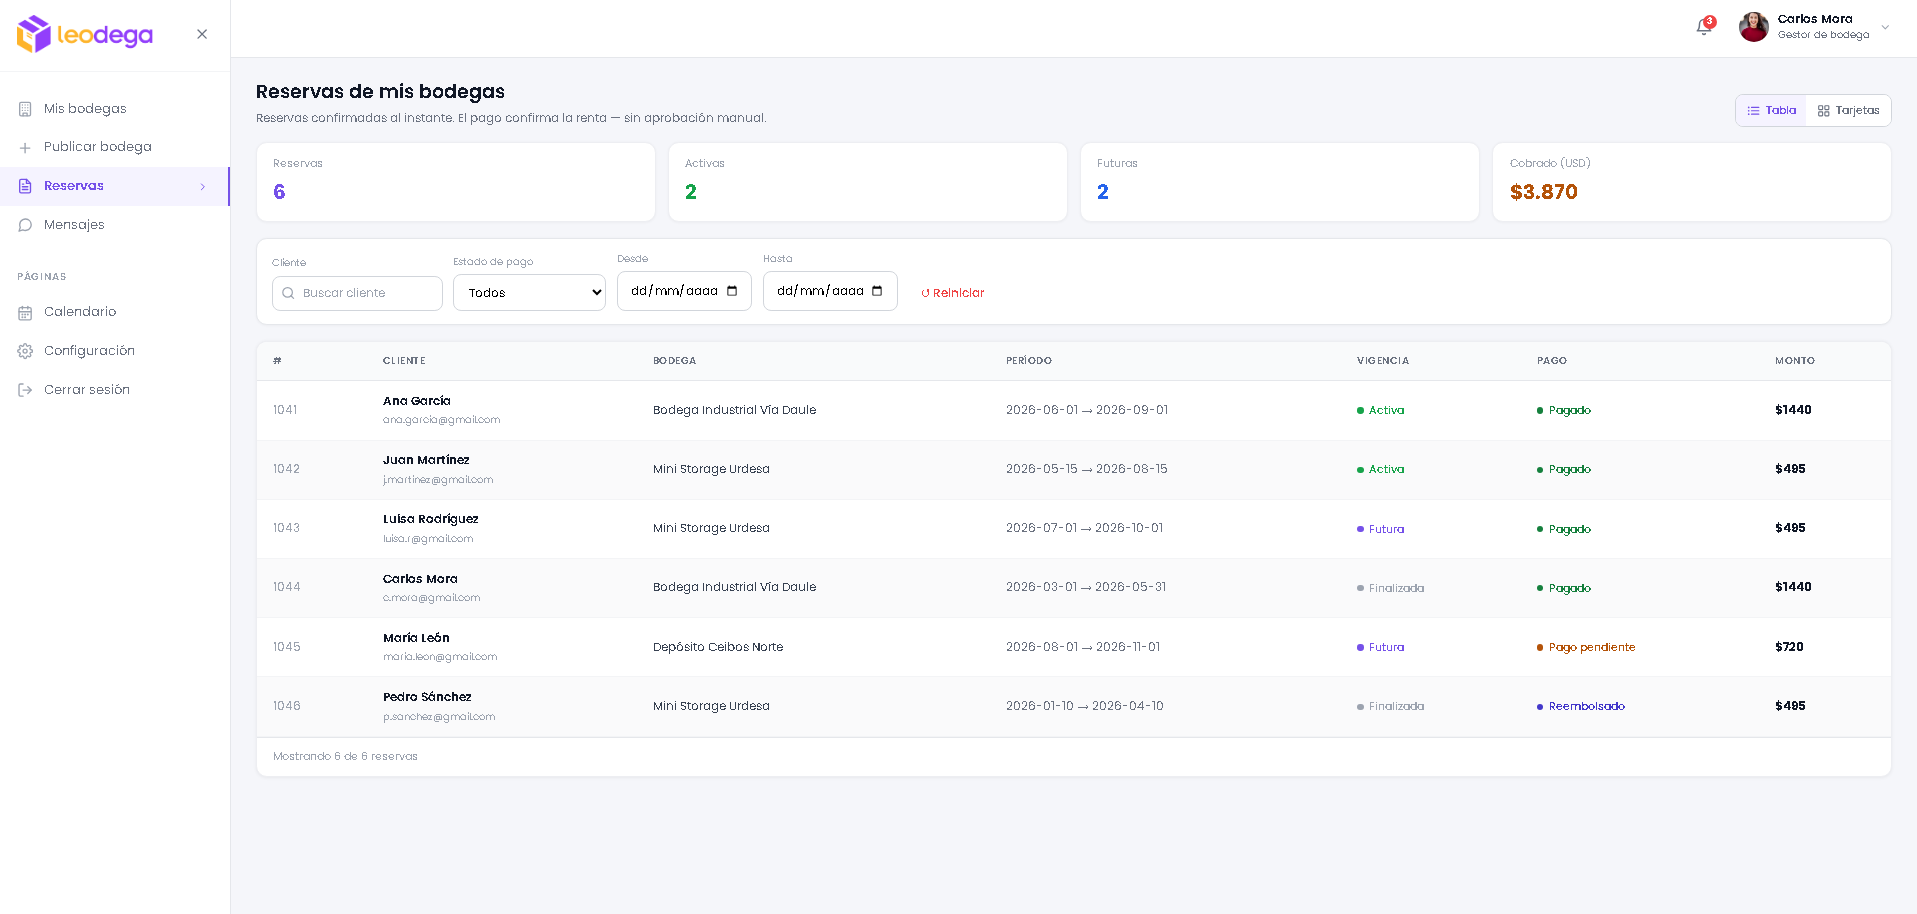
\includegraphics[width=\linewidth]{img/fig24_manager_bookings}
    \caption{Incoming Bookings: table with six bookings, key metrics,
    and payment status indicators.}
    \label{fig:manager_bookings}
\end{figure}

\subsection{Messages}

The manager's inbox organises conversations by client and warehouse,
distinguishing between pre-booking inquiries and active rental chats.

\begin{figure}[H]
    \centering
    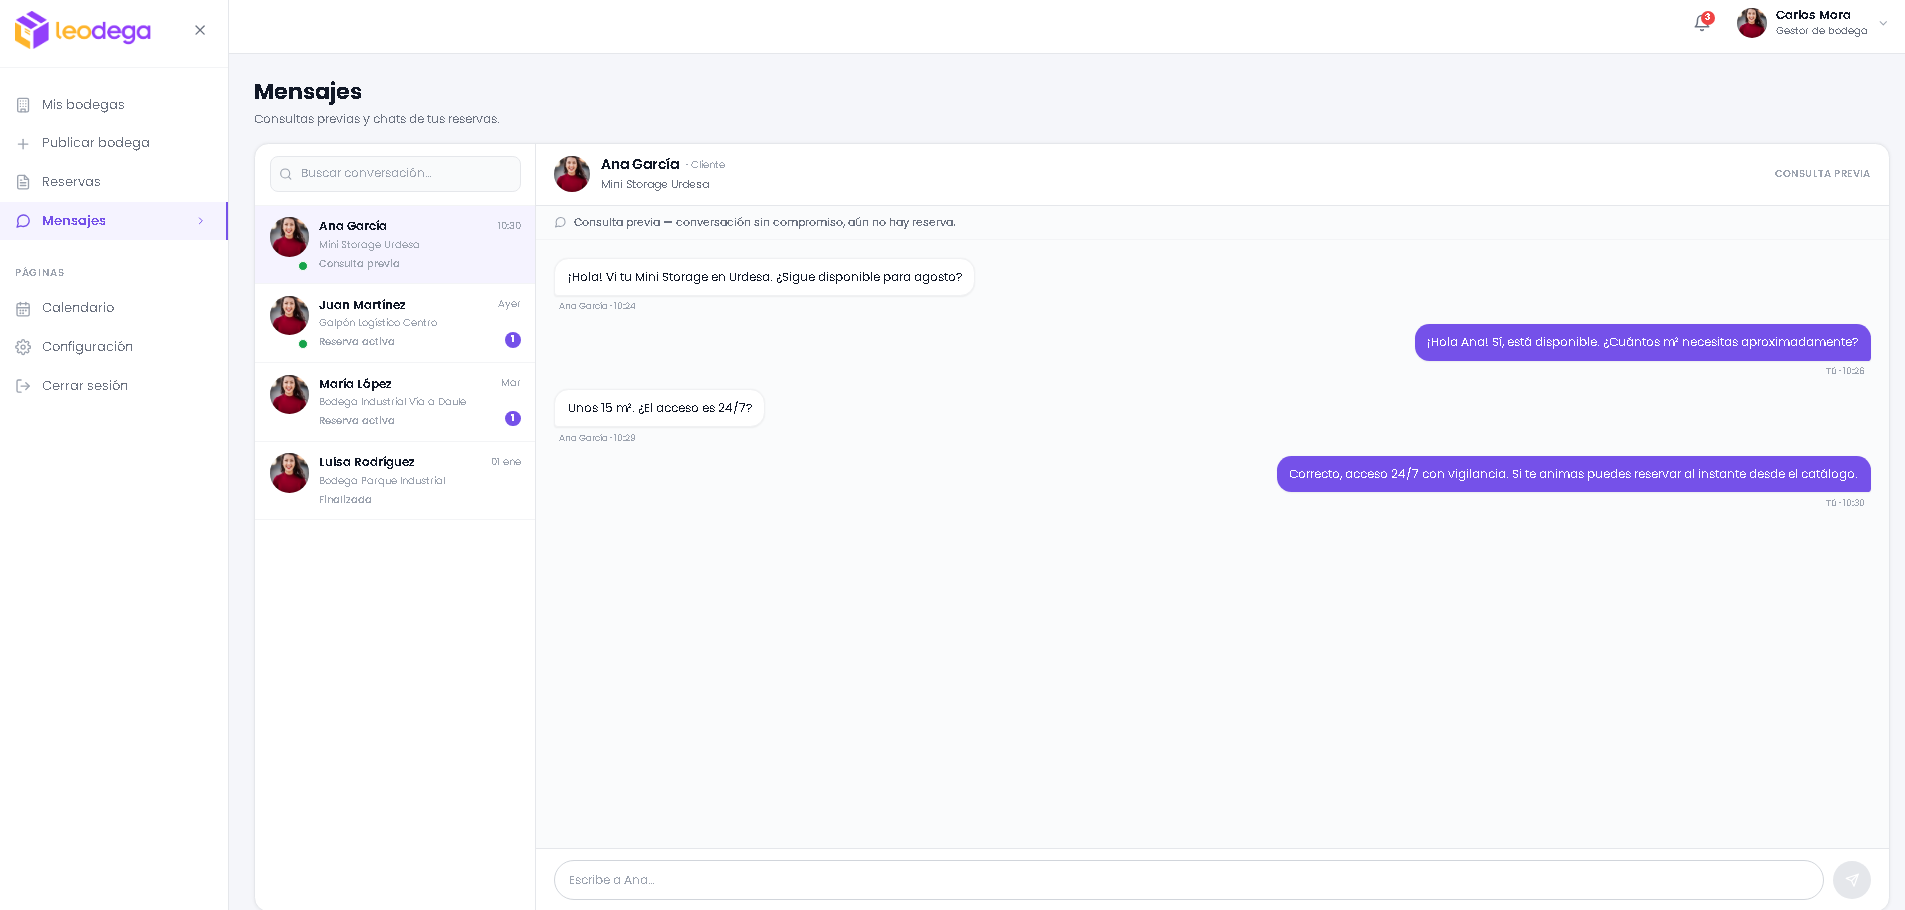
\includegraphics[width=\linewidth]{img/fig25_manager_messages}
    \caption{Manager Messages: client conversations organised by
    warehouse and booking status.}
    \label{fig:manager_messages}
\end{figure}

\subsection{Calendar}

Monthly calendar view displaying all bookings and pending payments,
colour-coded by status.

\begin{figure}[H]
    \centering
    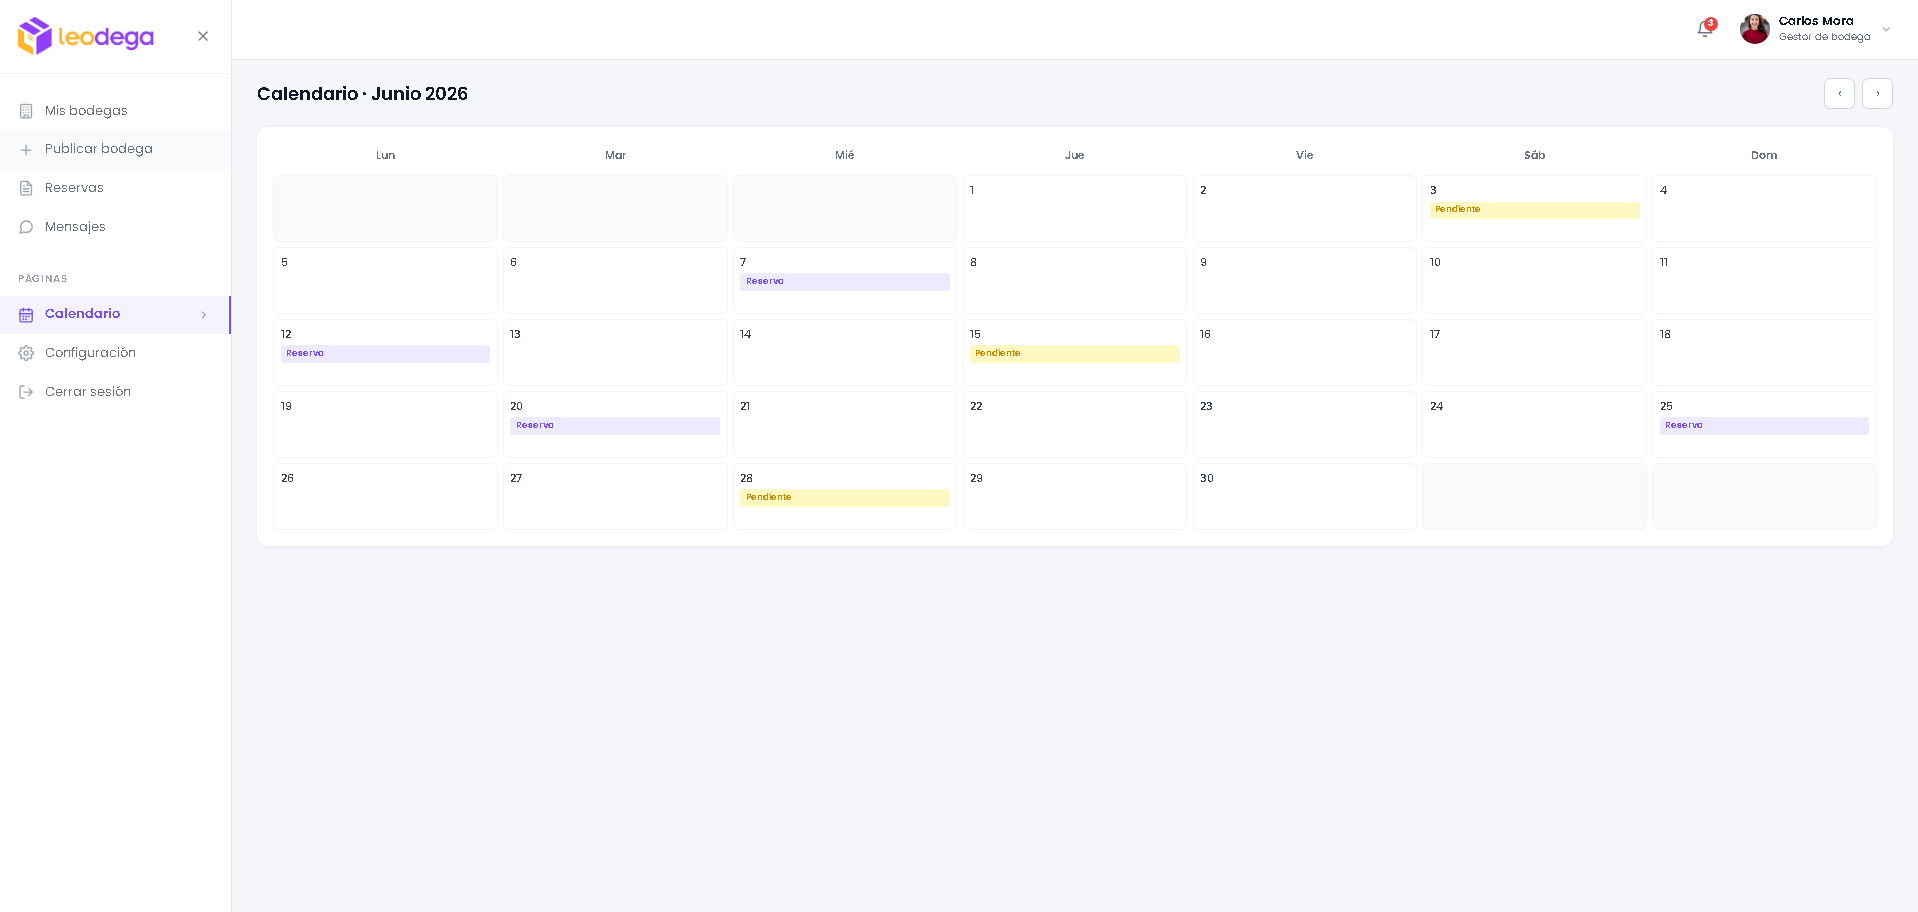
\includegraphics[width=\linewidth]{img/fig26_calendar}
    \caption{Calendar: monthly view (June 2026) with active bookings
    and pending payment events.}
    \label{fig:calendar}
\end{figure}

\subsection{Profile Settings}

Profile screen for updating personal information and switching the
panel view between available system roles.

\begin{figure}[H]
    \centering
    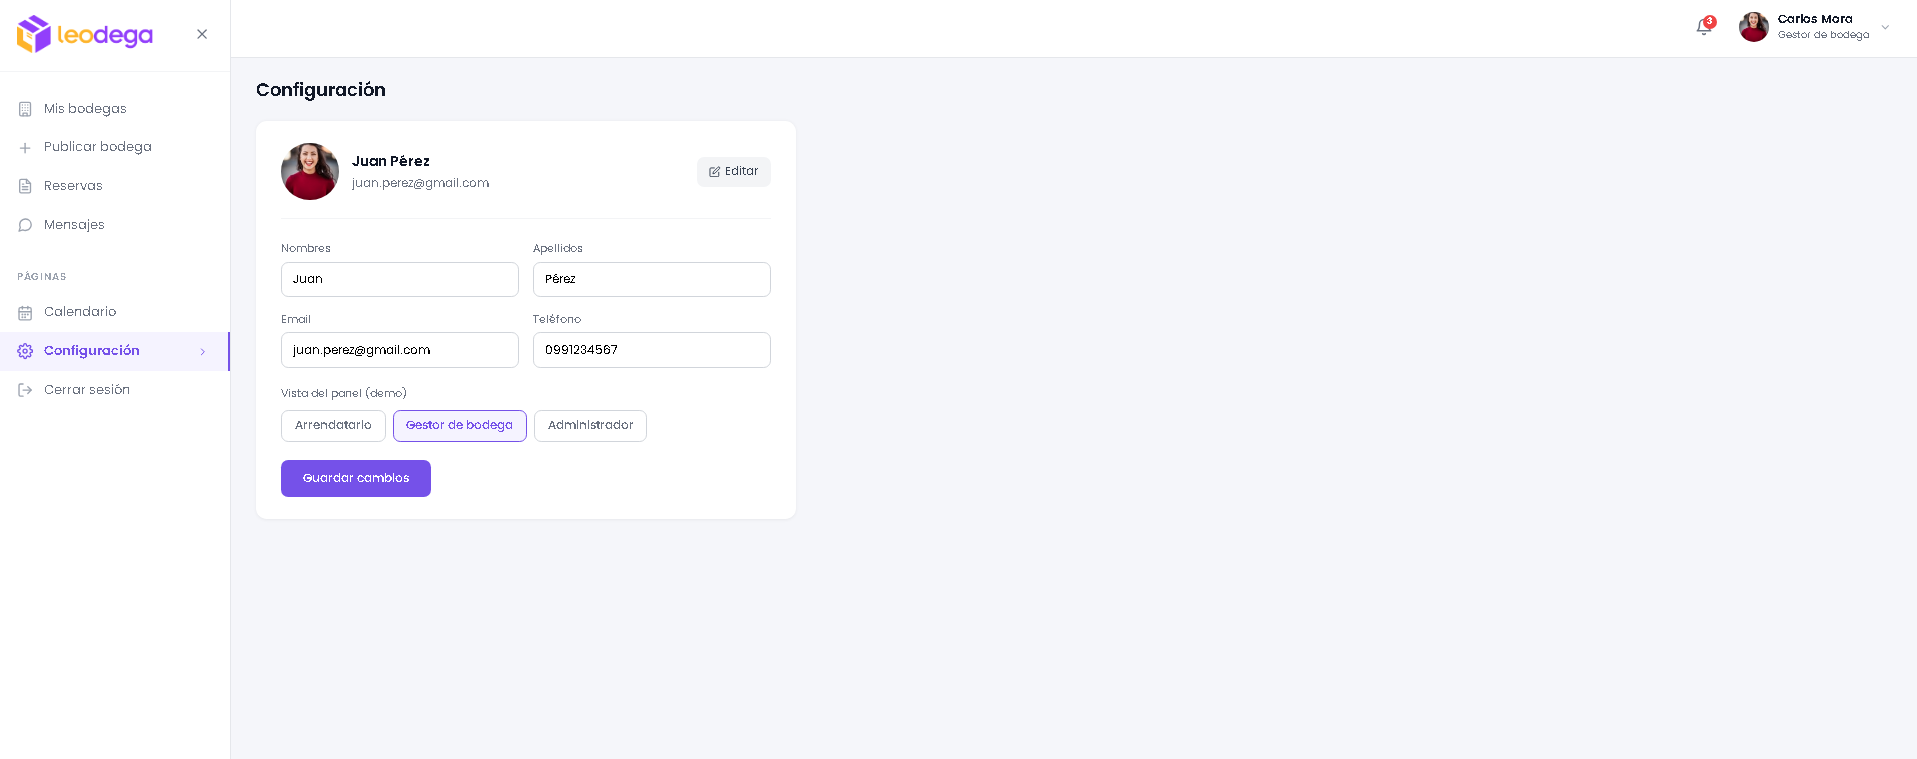
\includegraphics[width=0.55\linewidth]{img/fig27_manager_config}
    \caption{Profile Settings: personal data editor with role view
    selector.}
    \label{fig:manager_config}
\end{figure}

% ───────────────────────────────────────────────────────────────────
\section{Administrator}
% ───────────────────────────────────────────────────────────────────

The Administrator has full platform control: warehouse listing
approval, user account management, incident report tracking, and
direct messaging with participants.

\subsection{Dashboard}

Platform-wide metrics: active warehouses, pending approvals, monthly
bookings, and open reports, plus a pending listings queue and recent
activity log.

\begin{figure}[H]
    \centering
    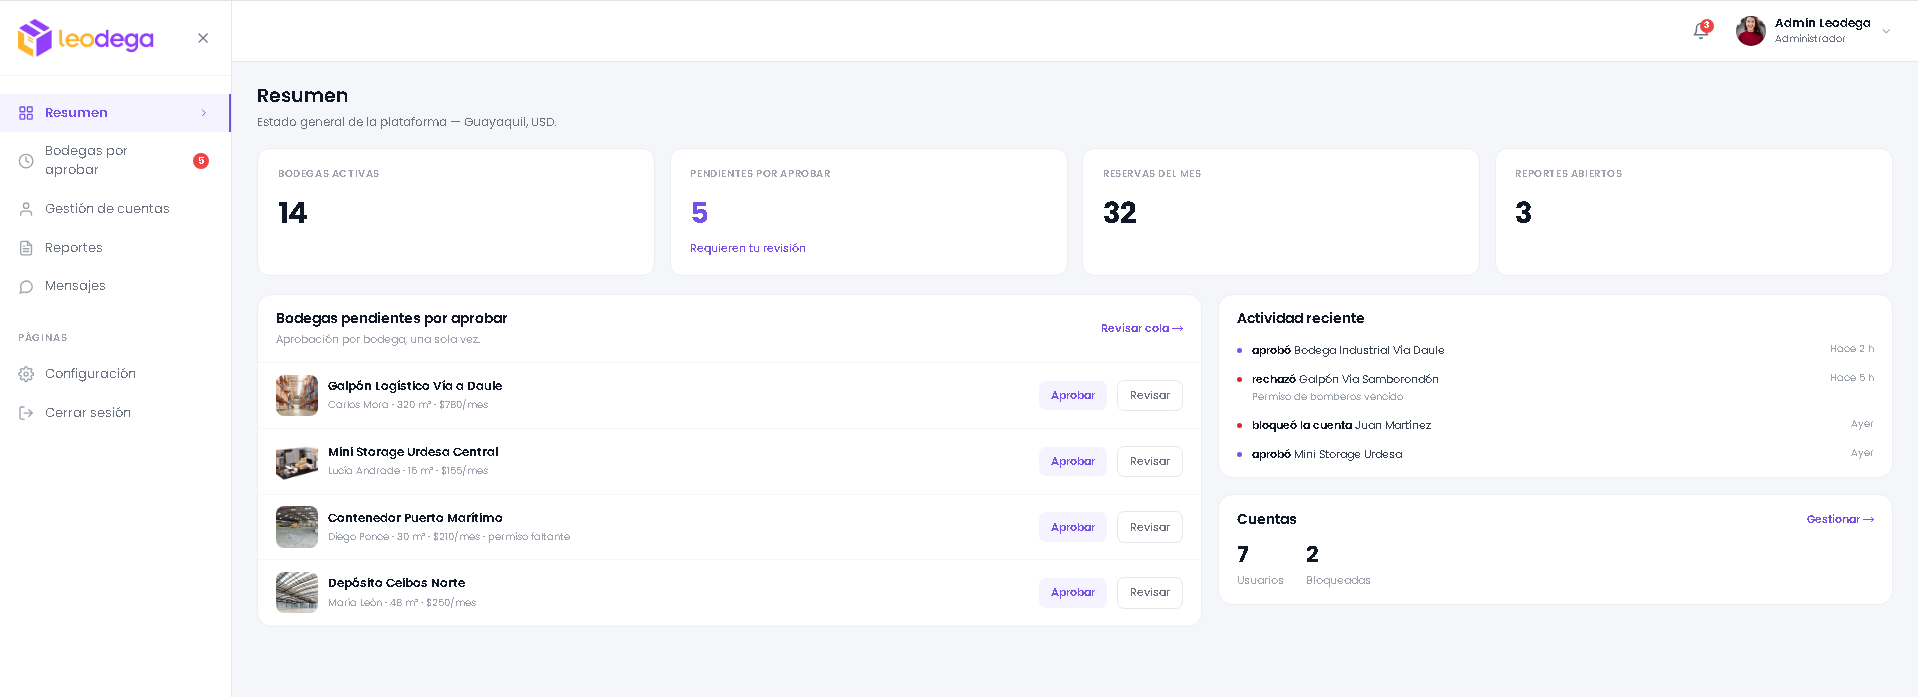
\includegraphics[width=\linewidth]{img/fig28_admin_dashboard}
    \caption{Admin Dashboard: platform overview showing 14 active
    warehouses, 5 pending approvals, 32 bookings, and 3 open reports.}
    \label{fig:admin_dashboard}
\end{figure}

\subsection{Warehouse Approval}

The approval queue presents submitted listings with photo galleries,
property details, and the fire department permit.

\begin{figure}[H]
    \centering
    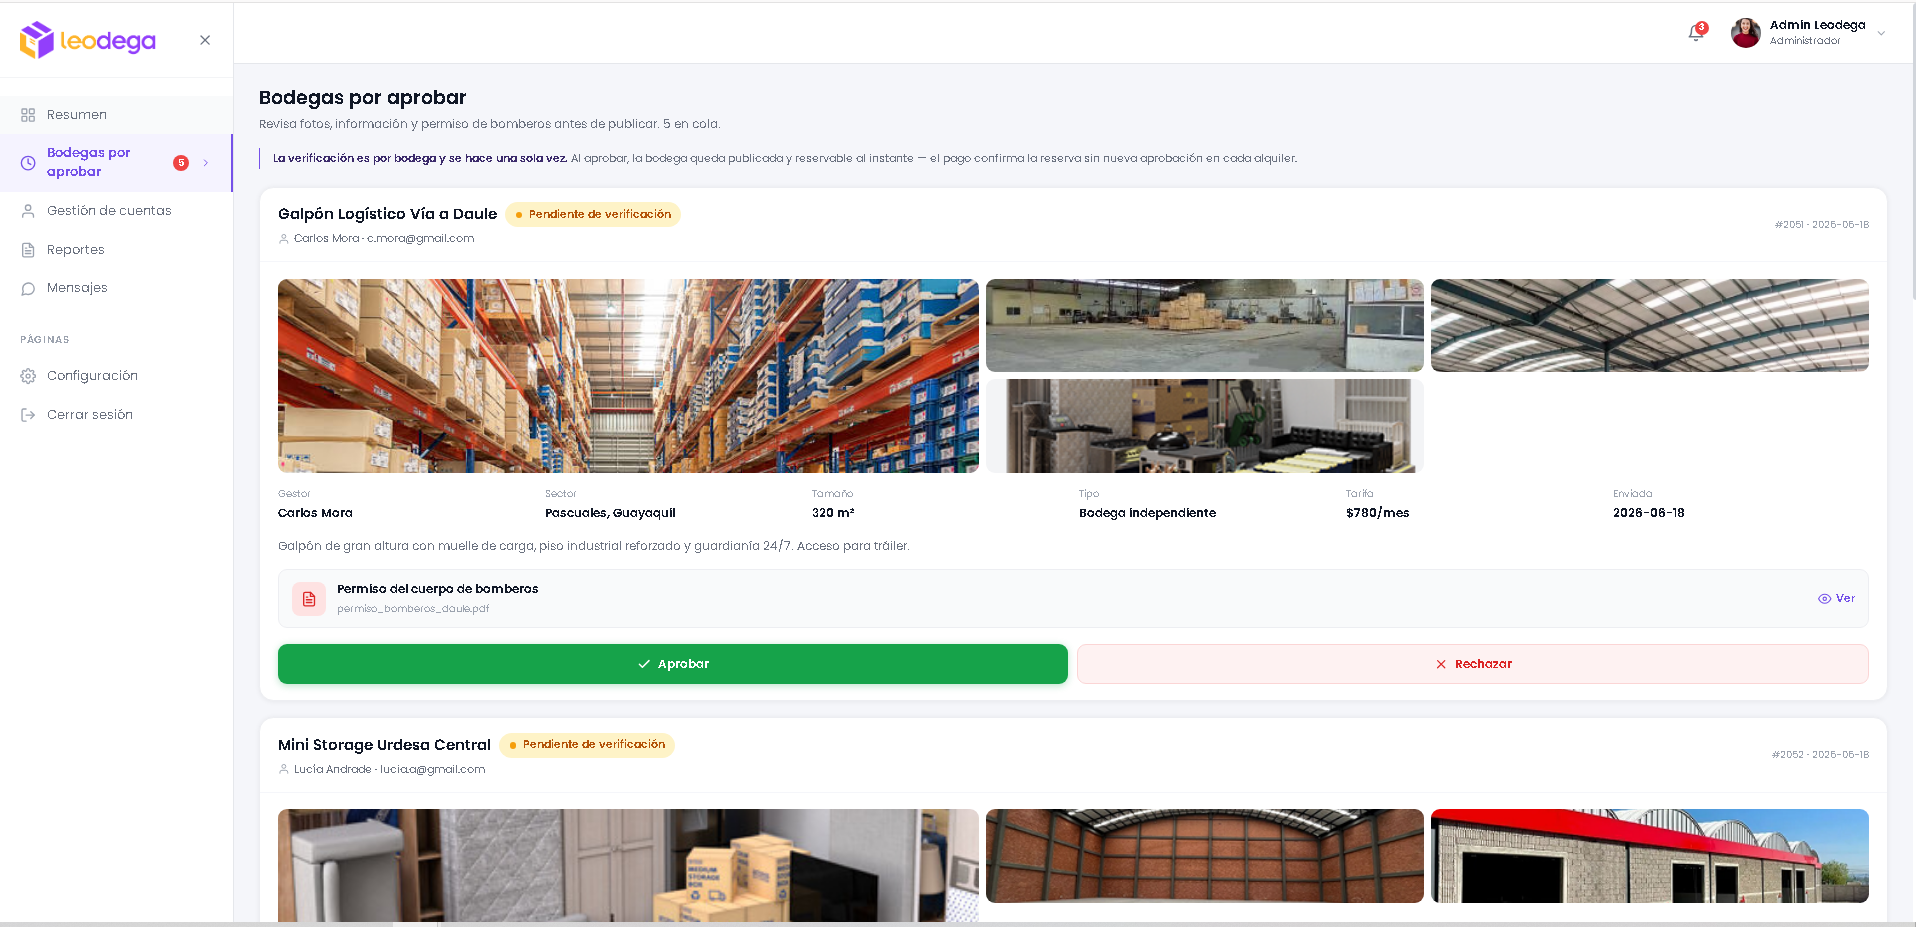
\includegraphics[width=\linewidth]{img/fig29_admin_approval}
    \caption{Warehouse Approval: review queue with photos, details,
    permit verification, and approve/reject actions.}
    \label{fig:admin_approval}
\end{figure}

\begin{figure}[H]
    \centering
    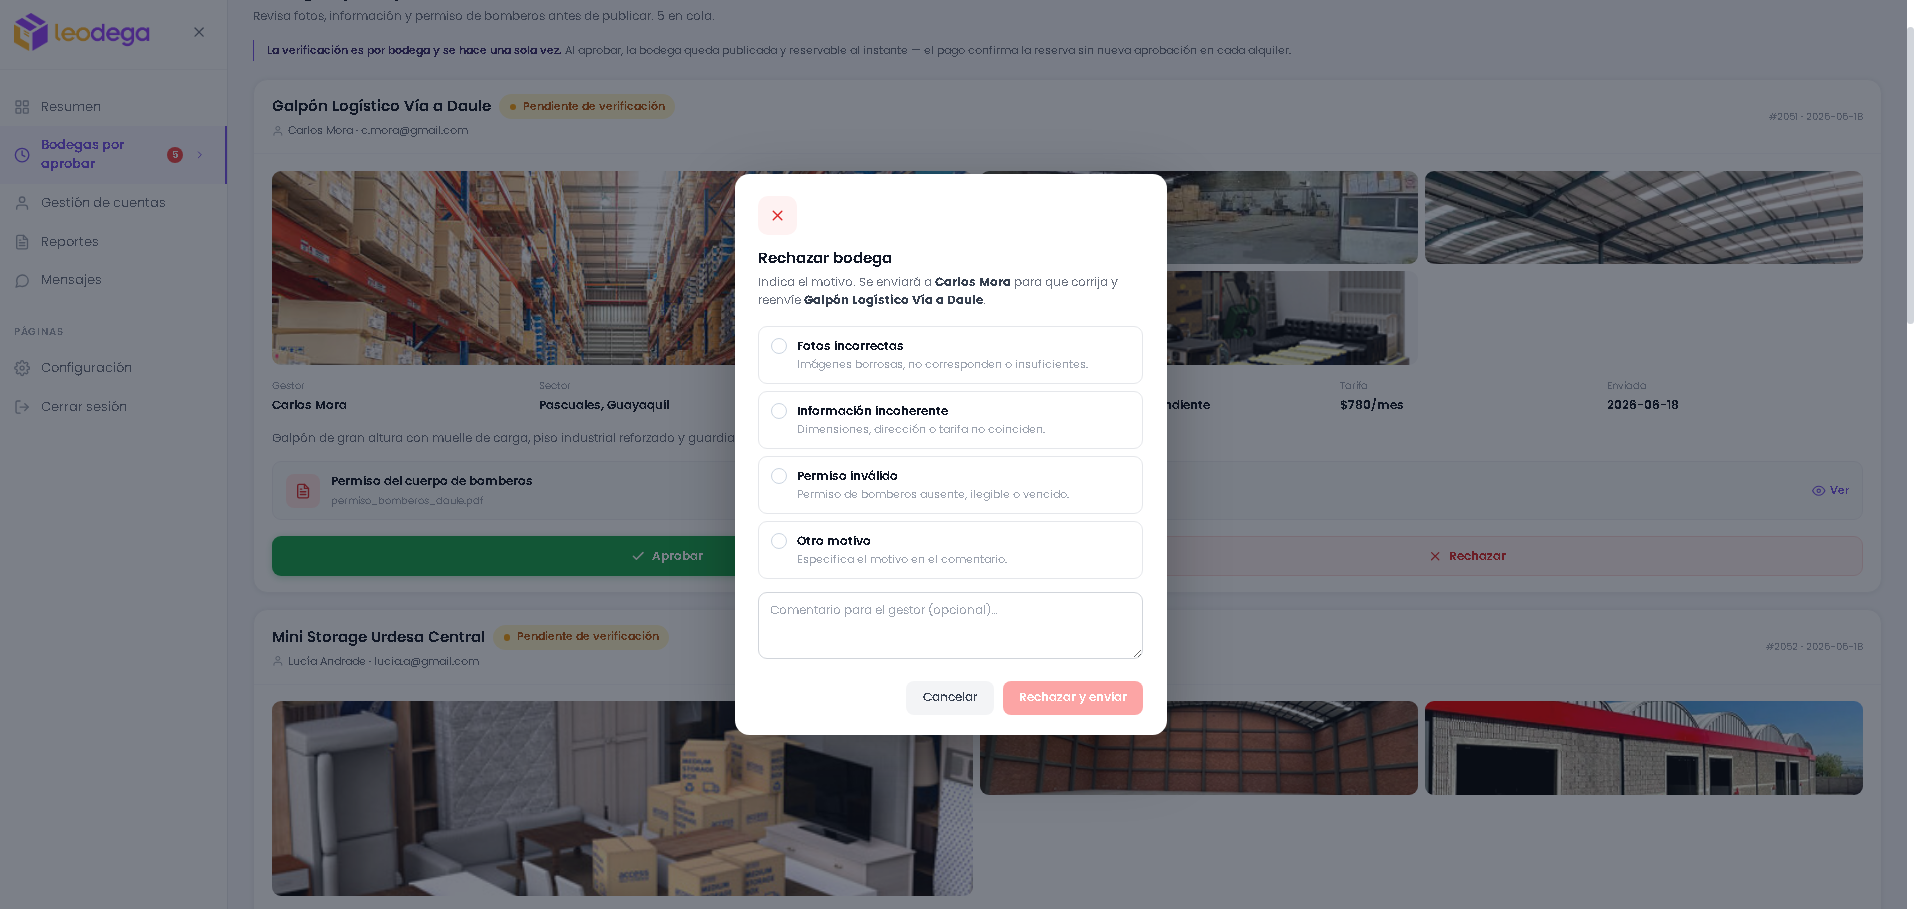
\includegraphics[width=\linewidth]{img/fig30_admin_reject_modal}
    \caption{Reject Warehouse Modal: rejection reason selection with
    optional comment sent to the manager.}
    \label{fig:admin_reject_modal}
\end{figure}

\subsection{Account Management}

Lists all registered accounts with role, registration date, warehouse
count, and status. The admin can block or reactivate accounts.

\begin{figure}[H]
    \centering
    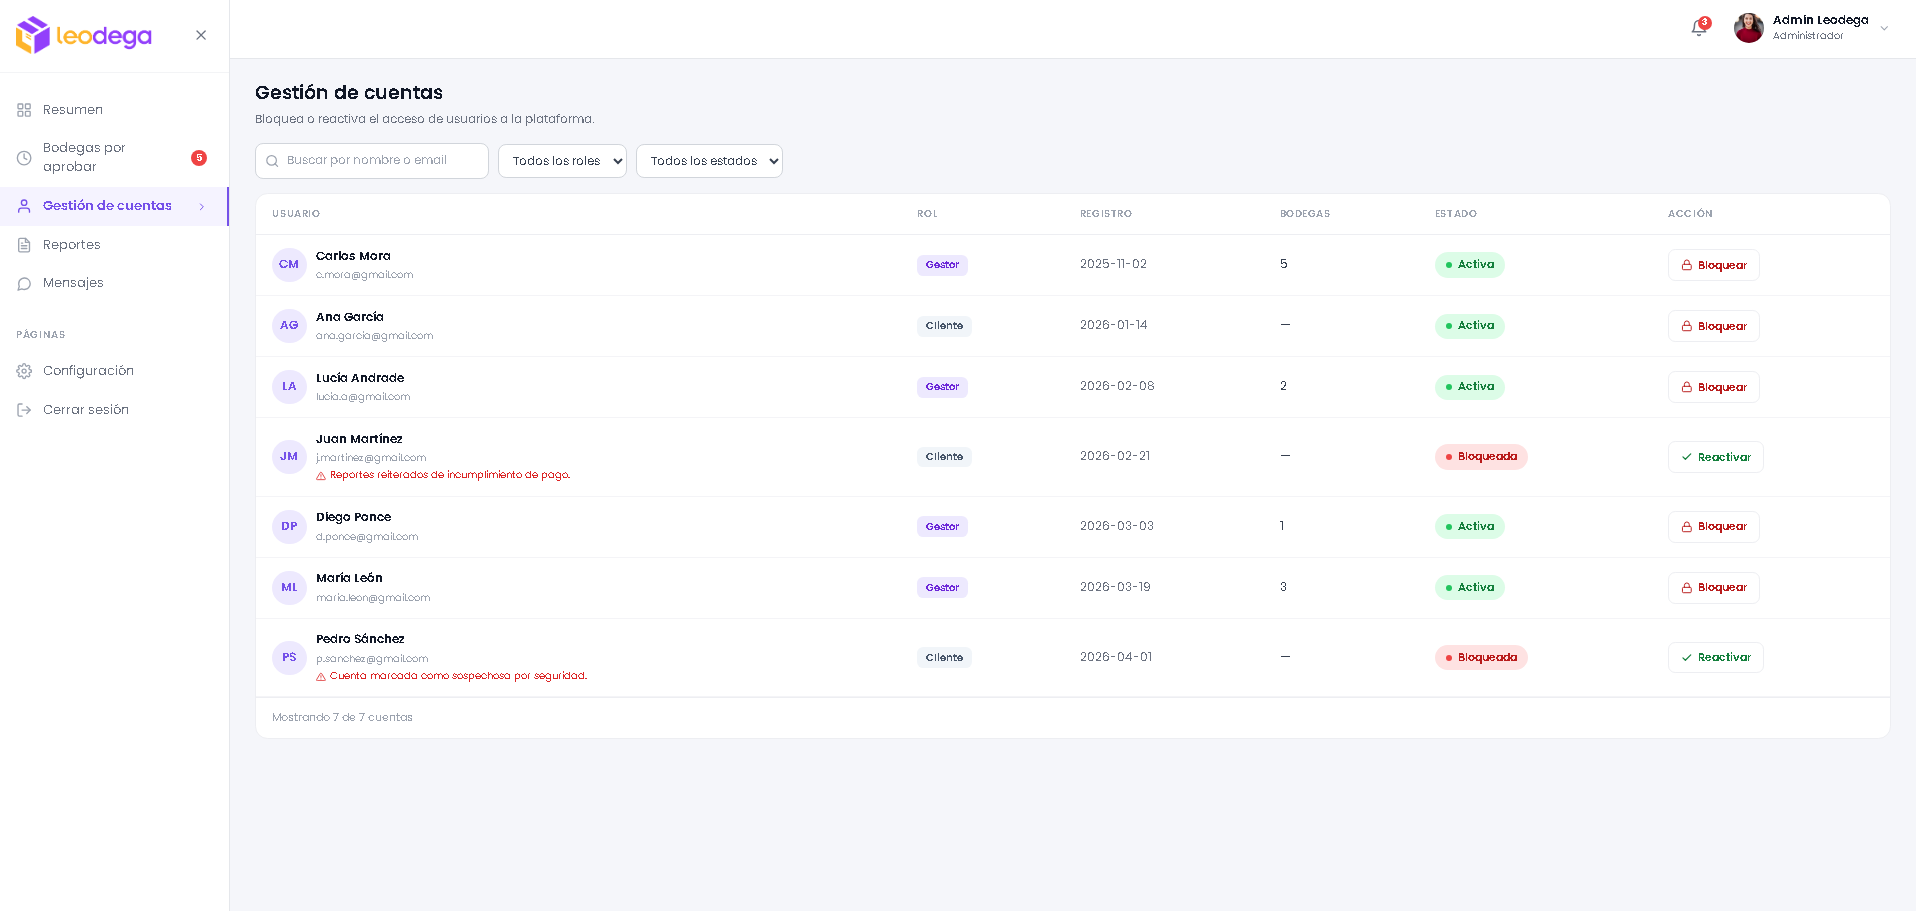
\includegraphics[width=\linewidth]{img/fig31_admin_accounts}
    \caption{Account Management: user table with role, registration
    date, warehouse count, and account status.}
    \label{fig:admin_accounts}
\end{figure}

\subsection{Reports}

Tracks platform incidents by type (Access, Security, Infrastructure)
and resolution status.

\begin{figure}[H]
    \centering
    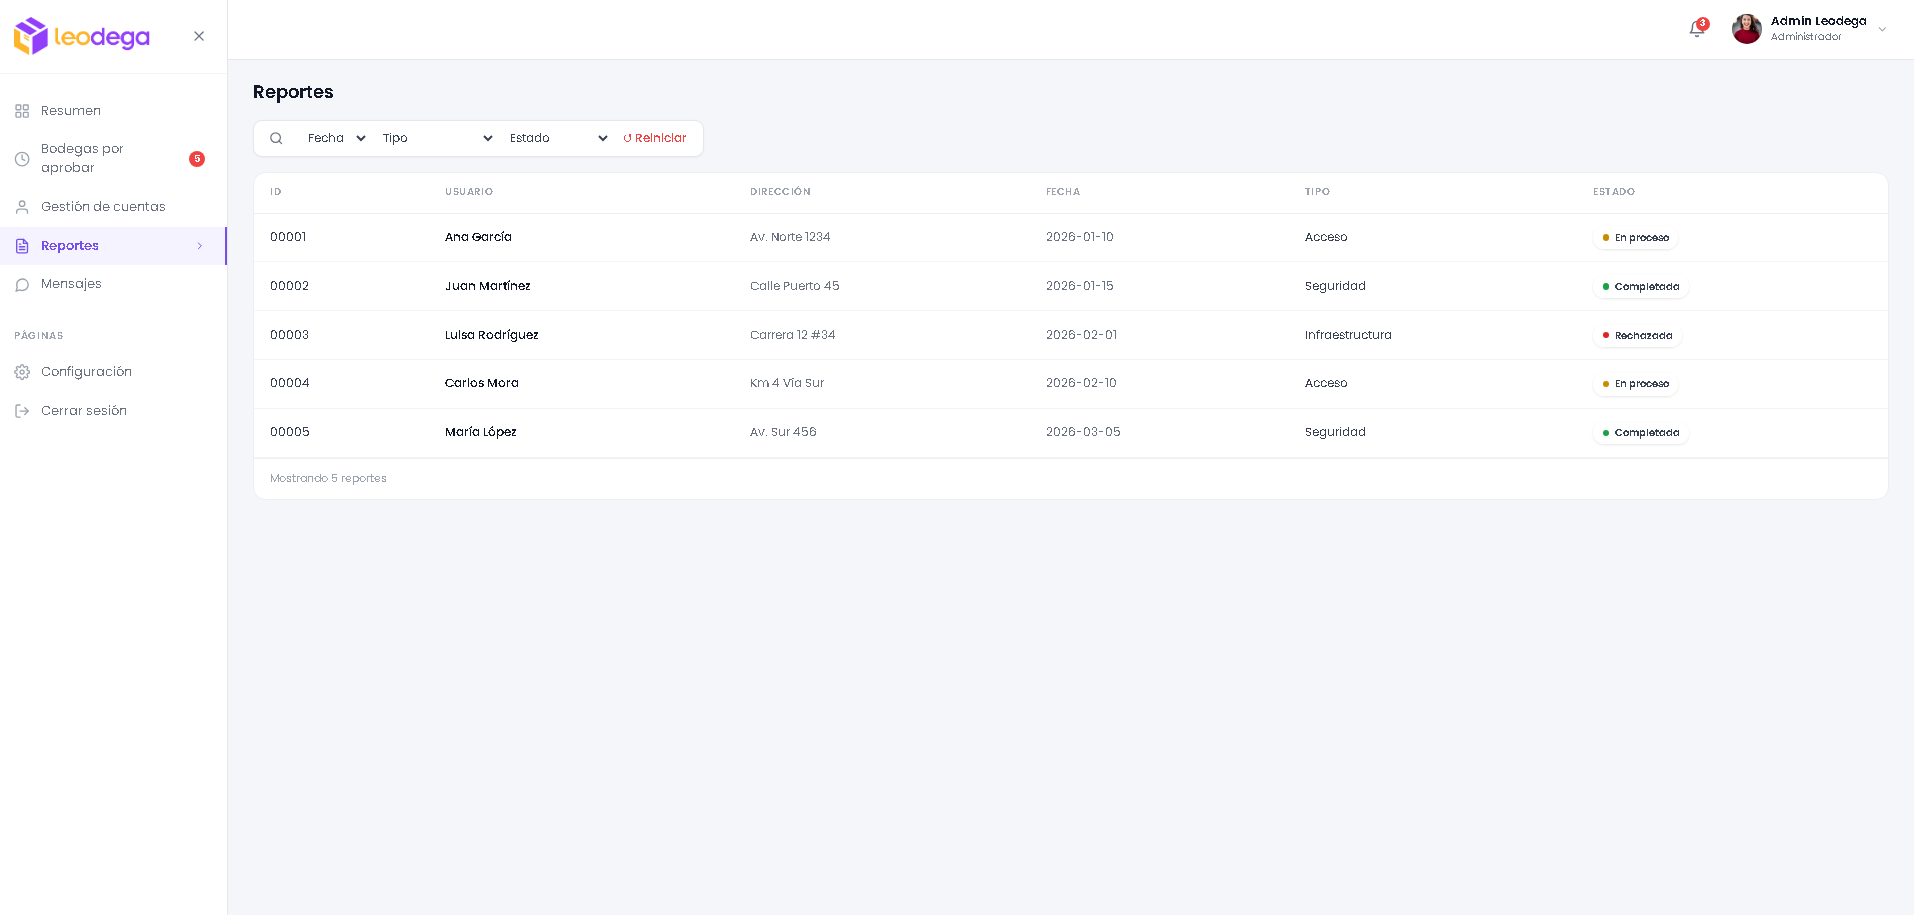
\includegraphics[width=\linewidth]{img/fig32_admin_reports}
    \caption{Reports: incident table with user, address, date, type,
    and resolution status.}
    \label{fig:admin_reports}
\end{figure}

\subsection{Messages}

Direct communication with platform users for support and moderation.

\begin{figure}[H]
    \centering
    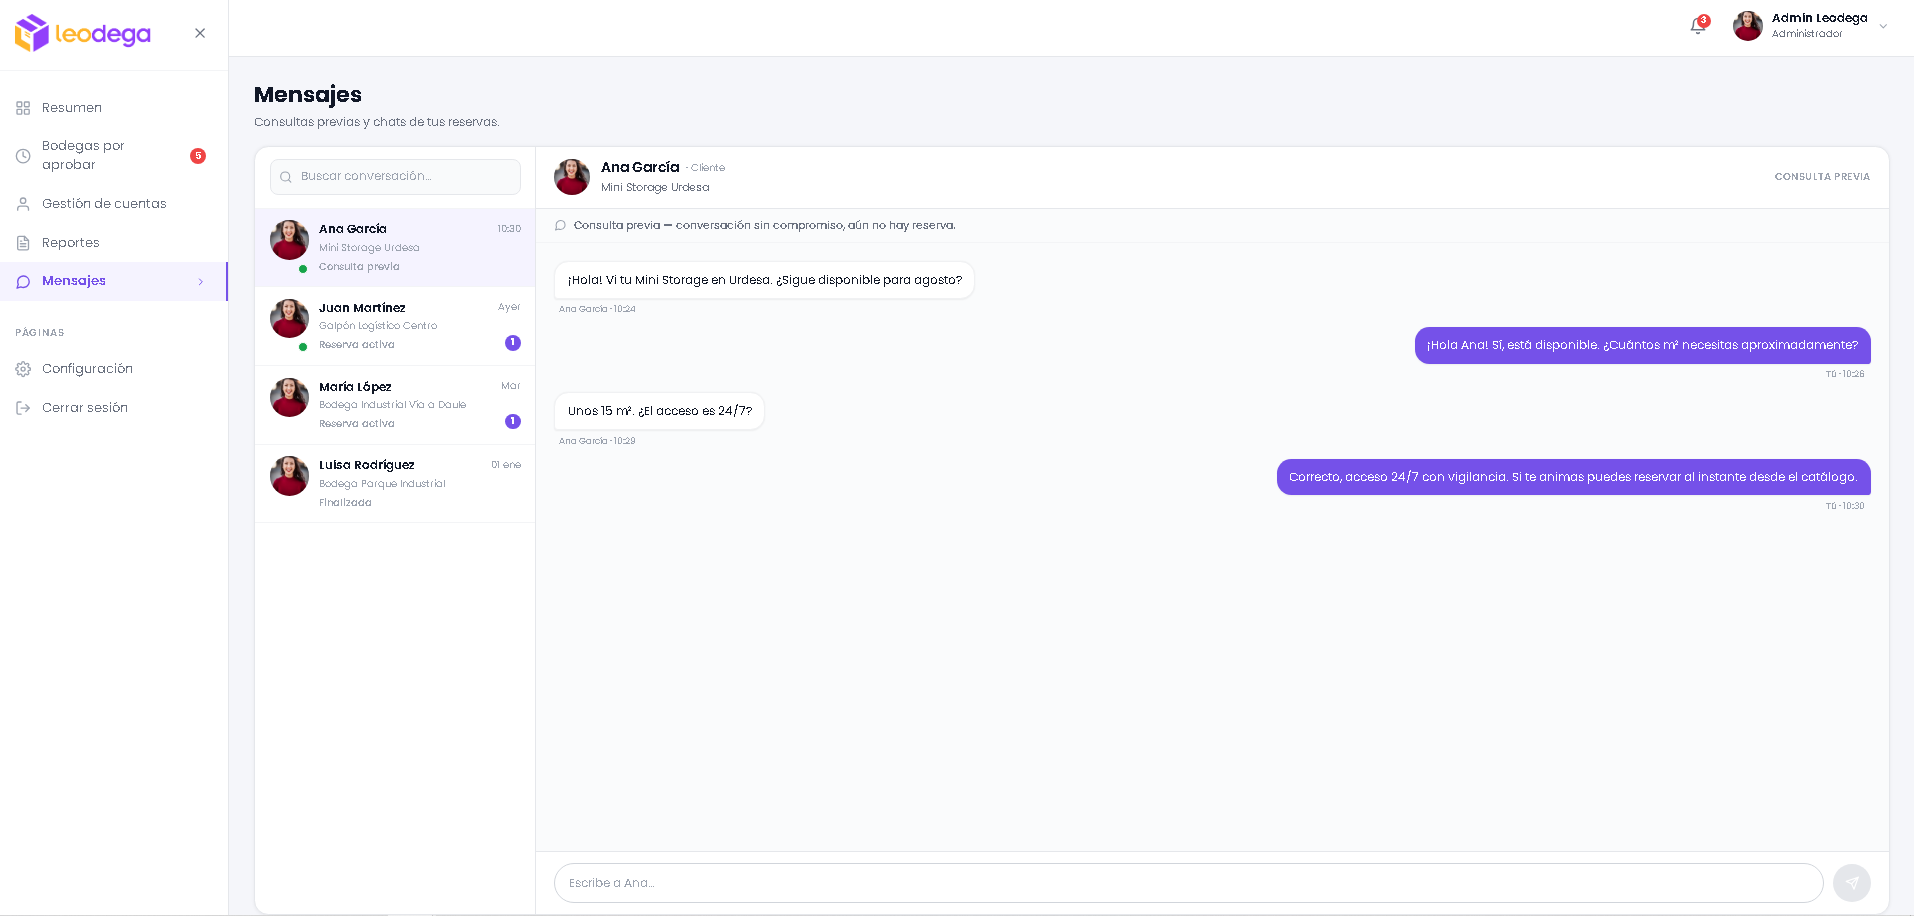
\includegraphics[width=\linewidth]{img/fig33_admin_messages}
    \caption{Admin Messages: inbox with user conversations for
    platform support and moderation.}
    \label{fig:admin_messages}
\end{figure}

\subsection{Profile Settings}

\begin{figure}[H]
    \centering
    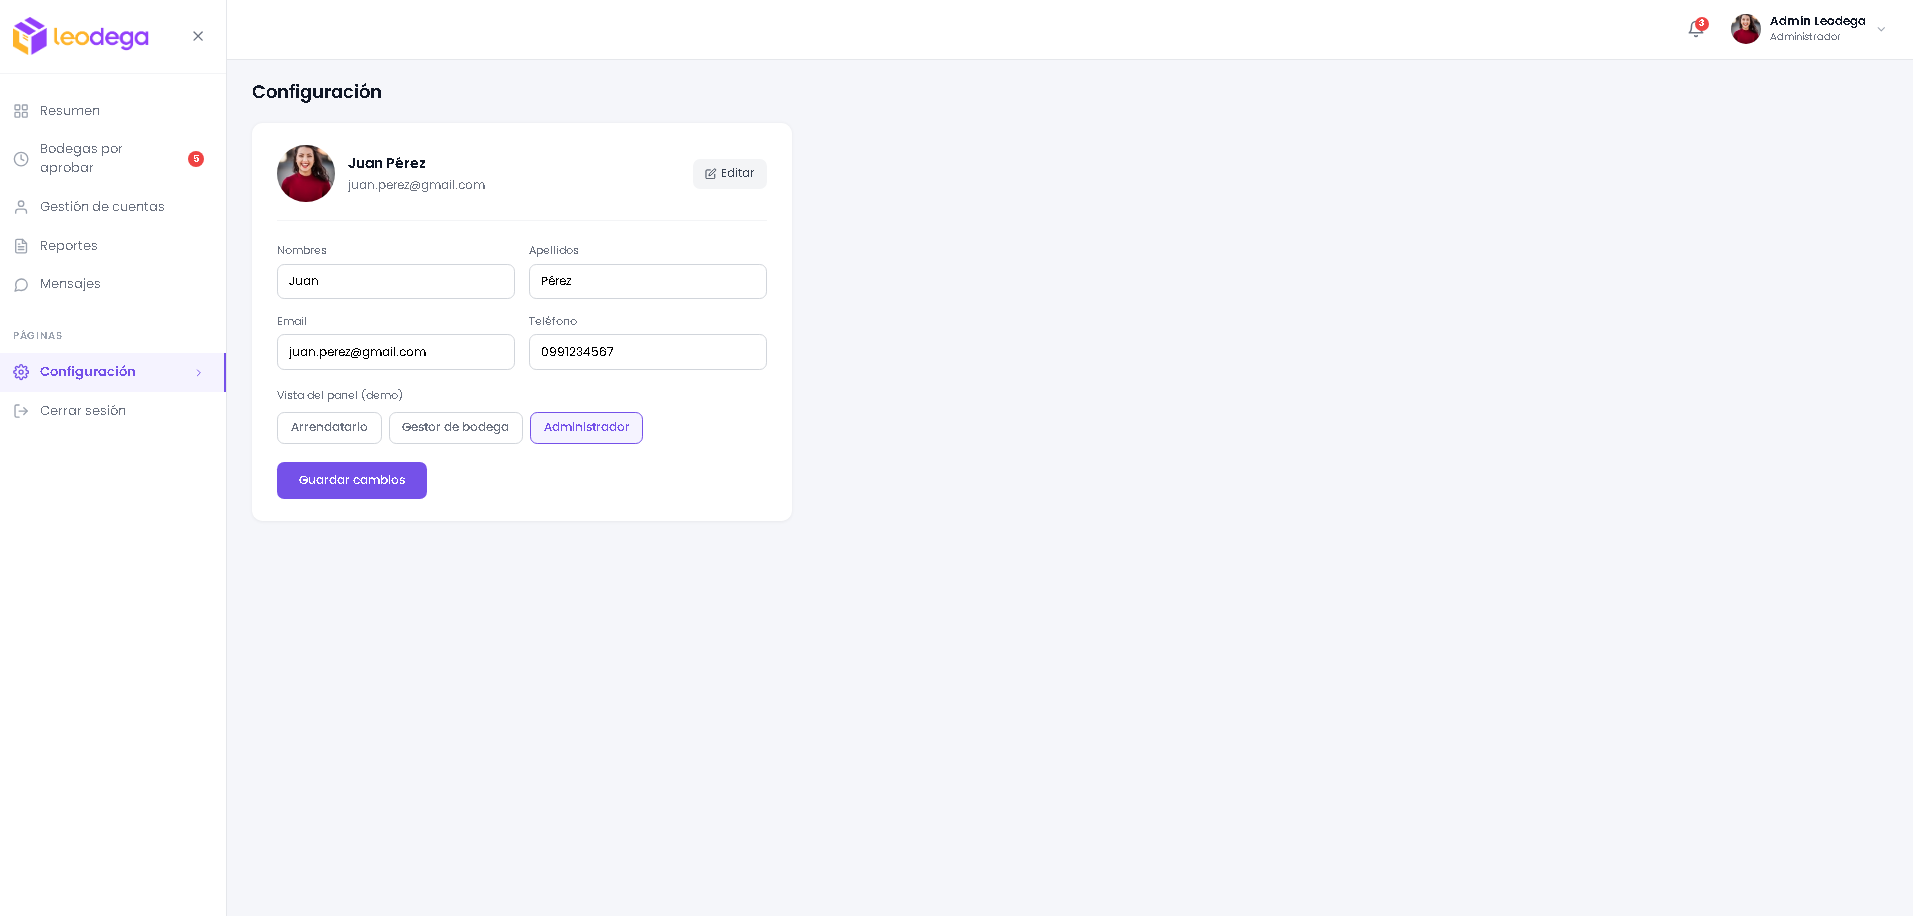
\includegraphics[width=0.55\linewidth]{img/fig34_admin_config}
    \caption{Admin Profile Settings: personal data editor with role
    view selector.}
    \label{fig:admin_config}
\end{figure}

\chapter{Acceptance Letter}

\begin{center}
    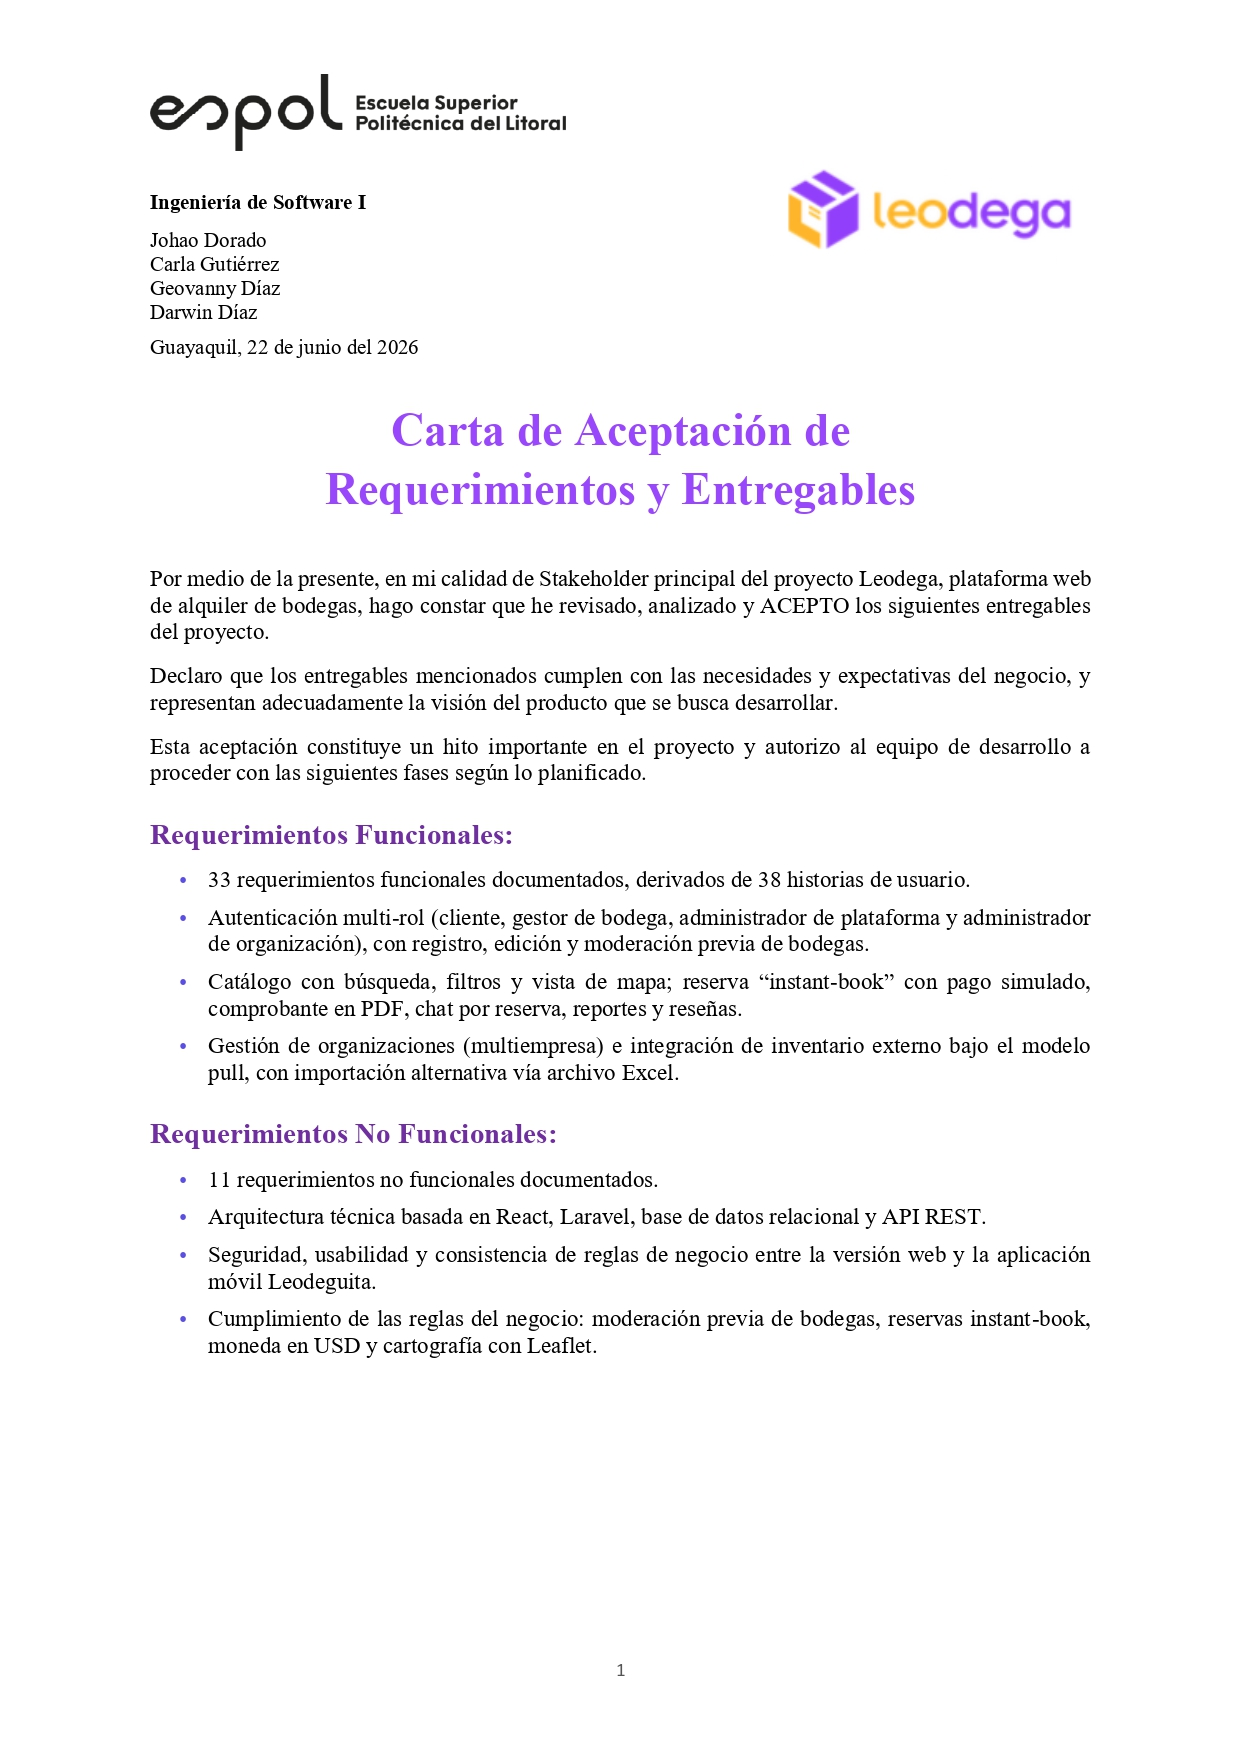
\includegraphics[width=0.9\textwidth]{CartaP1.jpg}
\end{center}

\vspace{0.5cm}

\begin{center}
    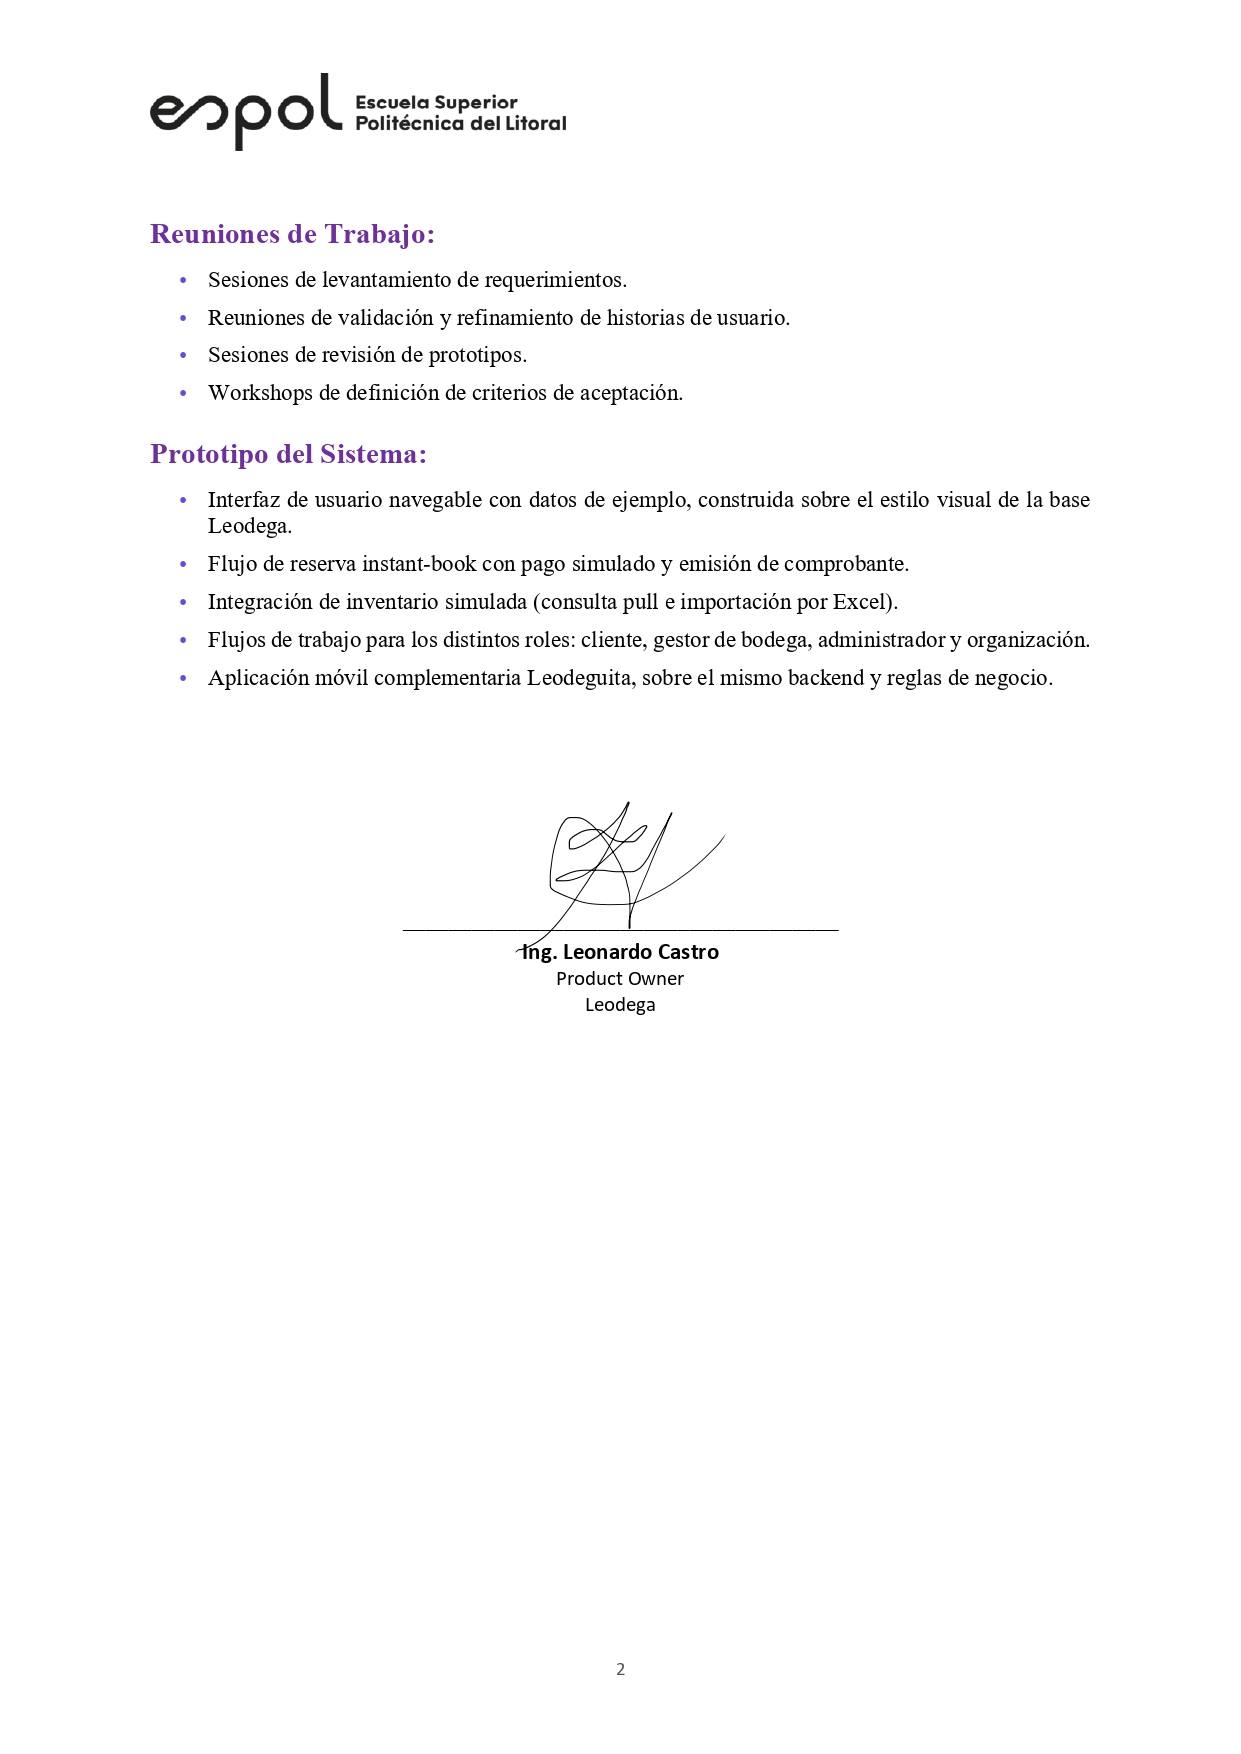
\includegraphics[width=0.9\textwidth]{CartaP2.jpg}
\end{center}
% =====================================================================
%  Appendices
%  Appendix A: User Stories (Functional Requirements)
%  Appendix B: Non-Functional Requirements
%  Sources: user_stories.md (App. A) and non_functional_requierements.md
%  (App. B). Format follows document_structure.md; editorial rules from
%  instructions.md and prompt.md (English, testable, IEEE-style,
%  Sommerville classification for NFRs, validation criteria for every
%  NFR).
% =====================================================================
\chapter{Links}

\begin{itemize}
    \item \textbf{Repositorio (Excel with user histories):} \url{https://espolec-my.sharepoint.com/:x:/g/personal/dldiaz_espol_edu_ec/IQBBQnkoG3uFRa2nX5pI2kURAa8pNF6cpxQ1POtHXTjjAUw?e=1B57HO}
    \item \textbf{Prototipo:} \url{https://darwin4050e.github.io/PrototipoLeodega/}
    \item \textbf{Project files (Folder with meet recording):} \url{https://espolec-my.sharepoint.com/:f:/g/personal/dldiaz_espol_edu_ec/IgCEzk7GtyQvTI93FPW-tZN4Aaz2tQWK37bkN083-wlybdM?e=1sSQTk}
\end{itemize}
\chapter{Product Owner Meeting Records}
Throughout the project, communication with the stakeholder took place through two main channels: Microsoft Teams and WhatsApp. This combination was necessary because the team members had conflicting schedules that made it difficult to coordinate frequent virtual meetings. Whenever availability allowed, the team held formal sessions over Microsoft Teams; otherwise, WhatsApp was used as a quicker alternative for brief questions or for staying in touch with the stakeholder between scheduled meetings.
\nopagebreak
\vspace{0.2cm}
\begingroup
\footnotesize
\renewcommand{\arraystretch}{0.95}
\begin{table}[htbp]
\centering
\caption{Meetings}
\begin{tabular}{|p{2.2cm}|p{1.2cm}|p{2.0cm}|p{0.9cm}|p{6.2cm}|}
\hline
\textbf{Channel} & \textbf{Date} & \textbf{Attendance} & \textbf{Time} & \textbf{Resume} \\
\hline
Microsoft Teams & May 21th & Complete & 27min & Leonardo introduced Leodega as a warehouse or inventory system for managing and renting storage spaces. He also noted API integrations, UI-based field mapping, and that the project is already in progress. \\
\hline
WhatsApp & May 22th & -- & -- & The client shared the deployment manuals from the previous project (Laravel and Frontend) as reference. \\
\hline
WhatsApp & May 24th & -- & -- & Request for administrator credentials to review the existing module and define what to improve or add. \\
\hline
WhatsApp & May 26th & -- & -- & Questions about the booking flow, how long a warehouse can stay in the system, and the business model. \\
\hline
Microsoft Teams & May 29th & Complete & 25min & Review of the project's user stories (Warehouse Manager, Client, Administrator) in the shared document. \\
\hline
WhatsApp & June 4th & -- & -- & Explanation of the multi-company scheme, the Leodega web platform and the ``Leodeguita'' mobile app share the same warehouse model and backend. \\
\hline
WhatsApp & June 7th & -- & -- & Resolution of the team's final doubts about the integration between Leodega and Leodeguita. \\
\hline
Microsoft Teams & June 22th & Complete & 40min & Review of the Leodega functional prototype (dashboard, messages, reservations) demonstrated live. \\
\hline
\end{tabular}
\end{table}
\endgroup
\appendix

% ---------------------------------------------------------------------
\chapter{User Stories (Functional Requirements)}
\label{app:user-stories}
% ---------------------------------------------------------------------

This appendix details the functional requirements of the Leodega platform as User Stories, following the format prescribed in \texttt{document\_structure.md}. Each story lists its identifier, priority (MoSCoW: \emph{Must}, \emph{Should}, \emph{Could}), estimation in story points, and the sprint in which it is planned; its statement in the canonical ``As a \dots, I want \dots, so that \dots'' form; and its acceptance criteria expressed as numbered scenarios of the form Context, Event, and Expected result. The requirements are grouped by the five roles that interact with the system: \emph{Storage Manager} (HUG), \emph{Client} (HUC), \emph{Administrator} (HUA), \emph{Organisation / Company} (HUE), and the \emph{Leodeguita} mobile companion (HUL). The user stories are the primary source of functional requirements of this specification.

% =====================================================================
\section{Storage Manager (HUG)}
% =====================================================================

\subsection{HUG-01 --- Pre-booking inquiry reception and reply}
\label{req:HUG-01}
\begin{description}
\item[Priority:] Could Have \quad \item[Estimate:] 5 points \quad \item[Sprint:] 4
\end{description}

\textbf{User story statement.} As a Storage Manager, I need to receive and reply to pre-booking inquiry messages from clients interested in my spaces, in order to provide timely information and build trust before the client makes a formal reservation.

\textbf{Acceptance criteria.}
\begin{enumerate}
\item \textbf{Scenario 1: New inquiry message received.} \emph{Context:} a client has sent an inquiry message about one of the Storage Manager's spaces. \emph{Event:} the system notifies the Manager about the new message. \emph{Expected result:} the system displays the notification in the Manager's panel with the client's name, the inquired space, and the message content, and the Manager can access the conversation thread from the notification.
\item \textbf{Scenario 2: Successful reply to the client's message.} \emph{Context:} the Manager accesses the message thread of an interested client and writes a reply. \emph{Event:} the Manager sends the reply message. \emph{Expected result:} the system registers and delivers the reply to the client, updates the conversation thread for both parties, and marks the inquiry as answered in the Manager's panel.
\item \textbf{Scenario 3: Unanswered inquiry after the time limit.} \emph{Context:} the Manager has one or more pending inquiries that have not been answered yet. \emph{Event:} the system detects that the time limit has elapsed without a reply. \emph{Expected result:} the system displays the unanswered inquiries highlighted as ``pending'', sorted from oldest to newest, so the Manager can prioritise replies. The prototype does not define an automatic deadline or penalty.
\end{enumerate}

\subsection{HUG-02 --- Payment-confirmation notification and contract activation}
\label{req:HUG-02}
\begin{description}
\item[Priority:] Should Have \quad \item[Estimate:] 3 points \quad \item[Sprint:] 2
\end{description}

\textbf{User story statement.} As a Storage Manager, I need to receive a notification when a client confirms payment for a reservation, in order to know in real time which contracts have been formalised and are ready to begin the rental period.

\textbf{Acceptance criteria.}
\begin{enumerate}
\item \textbf{Scenario 1: Successful confirmed payment notification.} \emph{Context:} a client has completed the payment process for a reservation on one of the Manager's spaces. \emph{Event:} the system registers the client's payment confirmation. \emph{Expected result:} the system sends a notification to the Manager with the client name, reserved space, amount paid, and contract dates, and the contract becomes active in the Manager's panel.
\item \textbf{Scenario 2: Payment not received after the deadline.} \emph{Context:} the client started a reservation on one of the Manager's spaces but did not complete the payment within the hold time. \emph{Event:} the system detects that the payment time limit has expired without confirmation. \emph{Expected result:} the system does not finalise the reservation, returns the space to the available state, and notifies the Manager that the space is free again.
\item \textbf{Scenario 3: Viewing the active contract in the panel.} \emph{Context:} the Manager accesses the contracts panel after receiving the confirmed payment notification. \emph{Event:} the Manager opens the active contracts section. \emph{Expected result:} the system displays the contract with all its details (client, space, dates, amount, and ``Active'' status), and the Manager can access the client's chat from the same panel.
\end{enumerate}

\subsection{HUG-03 --- Active-contract chat with clients}
\label{req:HUG-03}
\begin{description}
\item[Priority:] Could Have \quad \item[Estimate:] 5 points \quad \item[Sprint:] 4
\end{description}

\textbf{User story statement.} As a Storage Manager, I need to have an active chat channel with my clients during the current rental period, in order to coordinate access, resolve incidents, and maintain direct communication without leaving the platform.

\textbf{Acceptance criteria.}
\begin{enumerate}
\item \textbf{Scenario 1: Sending a message to a client with an active contract.} \emph{Context:} the Manager has an active contract with a client and wants to send them a message from the contracts panel. \emph{Event:} the Manager writes and sends the message in the contract chat. \emph{Expected result:} the system registers the message, delivers it to the client, and updates the chat thread with the send time, and the client receives a push or on-screen notification.
\item \textbf{Scenario 2: Receiving a message from the client with notification.} \emph{Context:} the client has sent a message to the Manager through the chat of an active contract. \emph{Event:} the client's message reaches the system. \emph{Expected result:} the system notifies the Manager with an alert indicating the client's name and the associated contract, and the Manager can reply directly from the notification or from the contracts panel.
\item \textbf{Scenario 3: Attempt to chat in a finished contract.} \emph{Context:} the Manager tries to send a message to a client whose rental contract has already ended. \emph{Event:} the Manager tries to write in that contract's chat. \emph{Expected result:} the system disables the text field and displays: ``This chat is not available because the rental period has ended.'' The history remains visible in read-only mode.
\end{enumerate}

\subsection{HUG-04 --- Warehouse registration with fire department permit}
\label{req:HUG-04}
\begin{description}
\item[Priority:] Must Have \quad \item[Estimate:] 5 points \quad \item[Sprint:] 1
\end{description}

\textbf{User story statement.} As a Storage Manager, I need to register a new warehouse on the platform, including dimensions, location, photos, monthly rate, and the valid fire department permit, in order to offer my space available for rent.

\textbf{Acceptance criteria.}
\begin{enumerate}
\item \textbf{Scenario 1: Successful warehouse registration without additional permits upload.} \emph{Context:} the Manager accesses the warehouse registration form and has all the required space information. \emph{Event:} the Manager completes all required fields, attaches the valid fire department permit, and submits the form. \emph{Expected result:} the system validates the data, stores the permit alongside the warehouse, creates it with ``pending verification'' status, sends it to the Administrator for review, and shows a success message.
\item \textbf{Scenario 2: Registration with permits upload.} \emph{Context:} the Manager is completing the registration form for a new warehouse. \emph{Event:} the Manager completes the required fields but does \emph{not} attach the fire department permit and submits the form. \emph{Expected result:} the system blocks the submission, does not create the warehouse, and displays the message: ``You must attach the valid fire department permit to continue.''
\item \textbf{Scenario 3: Attempt to register with missing required fields.} \emph{Context:} the Manager leaves one or more required fields incomplete. \emph{Event:} the Manager omits a required field. \emph{Expected result:} the system displays an error message indicating the required fields and does not allow submitting the form.
\end{enumerate}

\subsection{HUG-05 --- Reservation list viewing, filtering, and detail}
\label{req:HUG-05}
\begin{description}
\item[Priority:] Must Have \quad \item[Estimate:] 3 points \quad \item[Sprint:] 2
\end{description}

\textbf{User story statement.} As a Storage Manager, I need to view all reservations made for my warehouses, with details of dates, client, and payment status, in order to manage the use of my space and plan logistics.

\textbf{Acceptance criteria.}
\begin{enumerate}
\item \textbf{Scenario 1: Viewing the reservation list.} \emph{Context:} the Manager has at least one published warehouse with registered reservations. \emph{Event:} the Manager accesses the reservations module on the web page. \emph{Expected result:} the system displays a table with all reservations for their warehouses, including client, warehouse, start and end date, status (paid or canceled), and amount.
\item \textbf{Scenario 2: Filtering and searching reservations.} \emph{Context:} the Manager is viewing the reservation list and wants to narrow down the results. \emph{Event:} the Manager uses filters by date range, reservation status, or client name. \emph{Expected result:} the system updates the list showing only the reservations that match the selected criteria.
\item \textbf{Scenario 3: Viewing a reservation's detail.} \emph{Context:} the Manager is viewing the reservation list and wants to see the detail of a particular reservation. \emph{Event:} the Manager clicks on a specific reservation. \emph{Expected result:} the system opens a detailed view with the complete client information and the payment receipt.
\end{enumerate}

\subsection{HUG-06 --- Cancellation of paid future reservations}
\label{req:HUG-06}
\begin{description}
\item[Priority:] Must Have \quad \item[Estimate:] 3 points \quad \item[Sprint:] 2
\end{description}

\textbf{User story statement.} As a Storage Manager, I need to cancel a previously paid reservation, indicating a mandatory reason, in order to free up my space in case of unforeseen events and maintain transparency with the client.

\textbf{Acceptance criteria.}
\begin{enumerate}
\item \textbf{Scenario 1: Successful cancellation of a future reservation.} \emph{Context:} the Manager has a paid reservation with a future start date on one of their warehouses. \emph{Event:} the Manager selects a paid reservation with a future start date, enters a valid reason, and confirms the cancellation. \emph{Expected result:} the system changes the reservation status to ``canceled by manager'', notifies the client via email, and frees the space for new reservations.
\item \textbf{Scenario 2: Cancellation of an already started or finished reservation.} \emph{Context:} the Manager has a paid reservation whose start date has already passed or that has already finished. \emph{Event:} the Manager tries to cancel that reservation. \emph{Expected result:} the system displays an error message indicating that it is not possible to cancel ongoing or finished reservations.
\item \textbf{Scenario 3: Cancellation without a reason.} \emph{Context:} the Manager selects a paid, future reservation and tries to cancel it. \emph{Event:} the Manager tries to cancel without filling in the mandatory reason field. \emph{Expected result:} the system does not allow the cancellation and highlights the reason field as required.
\end{enumerate}

\subsection{HUG-07 --- Warehouse deletion (no active or future reservations)}
\label{req:HUG-07}
\begin{description}
\item[Priority:] Must Have \quad \item[Estimate:] 3 points \quad \item[Sprint:] 1
\end{description}

\textbf{User story statement.} As a Storage Manager, I need to delete a warehouse from the platform, provided it has no active or future reservations, in order to remove spaces that I no longer offer for rent.

\textbf{Acceptance criteria.}
\begin{enumerate}
\item \textbf{Scenario 1: Successful deletion of a warehouse without reservations.} \emph{Context:} the Manager selects a warehouse they own that has no active or confirmed future reservations. \emph{Event:} the Manager selects ``Delete warehouse'' and confirms the action in the confirmation dialog. \emph{Expected result:} the system removes the warehouse from the public catalog and the Manager's listings, marks it as inactive while preserving its history, and displays ``The warehouse was deleted successfully.''
\item \textbf{Scenario 2: Attempt to delete a warehouse with active or future reservations.} \emph{Context:} the warehouse has at least one ongoing reservation or a confirmed/paid future reservation. \emph{Event:} the Manager tries to delete it. \emph{Expected result:} the system blocks the deletion and displays ``You cannot delete this warehouse because it has active or future reservations. Wait for them to end or manage them before deleting it'', without making any changes.
\item \textbf{Scenario 3: Deletion of a warehouse with only finished (historical) reservations.} \emph{Context:} the warehouse only has already finished reservations, with none active or future. \emph{Event:} the Manager confirms the deletion. \emph{Expected result:} the system allows the operation but preserves the history of finished reservations for audit and reporting purposes; the warehouse is marked as inactive instead of being physically deleted.
\end{enumerate}

\subsection{HUG-08 --- Warehouse information editing}
\label{req:HUG-08}
\begin{description}
\item[Priority:] Must Have \quad \item[Estimate:] 5 points \quad \item[Sprint:] 1
\end{description}

\textbf{User story statement.} As a Storage Manager, I need to edit the information of a warehouse I have already published, such as dimensions, description, photos, monthly rate, and availability, in order to keep my space's offer up to date without having to delete and recreate it.

\textbf{Acceptance criteria.}
\begin{enumerate}
\item \textbf{Scenario 1: Successful warehouse data edit.} \emph{Context:} the Manager accesses a warehouse they own and modifies one or more of its editable fields. \emph{Event:} the Manager saves the changes with all valid data. \emph{Expected result:} the system validates the data, updates the warehouse information, reflects the changes in the catalog and the Manager's listings, and displays ``Changes were saved successfully.''
\item \textbf{Scenario 2: Attempt to save with missing or invalid required fields.} \emph{Context:} the Manager clears a required field or enters an invalid value (for example, a zero or negative rate). \emph{Event:} the Manager tries to save the changes. \emph{Expected result:} the system highlights the fields with errors, displays a validation message describing what to fix, and does not save any changes.
\item \textbf{Scenario 3: Editing a warehouse with active or future reservations.} \emph{Context:} the Manager modifies the rate or other data of a warehouse that already has confirmed or ongoing reservations. \emph{Event:} the Manager saves the changes. \emph{Expected result:} the system applies the changes only to new reservations; already confirmed reservations keep the conditions (rate and dates) they were agreed upon with, and the system informs the Manager that the changes do not affect existing contracts.
\end{enumerate}

% =====================================================================
\section{Client (HUC)}
% =====================================================================

\subsection{HUC-01 --- Warehouse search, filtering, and map view}
\label{req:HUC-01}
\begin{description}
\item[Priority:] Must Have \quad \item[Estimate:] 5 points \quad \item[Sprint:] 2
\end{description}

\textbf{User story statement.} As a client, I need to search and filter available warehouses by location, size, and price, in order to find the storage space that best fits my needs and budget without having to review all options manually.

\textbf{Acceptance criteria.}
\begin{enumerate}
\item \textbf{Scenario 1: Search with available results.} \emph{Context:} the client enters the warehouse catalog and applies location, minimum size, and price range filters. \emph{Event:} the client presses the search button with the selected filters. \emph{Expected result:} the system displays a list of approved warehouses that meet all the entered criteria, with their name, monthly price, size, and estimated distance, and each result includes a button to view the detail.
\item \textbf{Scenario 2: Search with no results for the applied filters.} \emph{Context:} the client applies filters whose combination does not match any available warehouse in the system. \emph{Event:} the client runs the search with those criteria. \emph{Expected result:} the system displays ``We didn't find available warehouses with those criteria. Try broadening your search'' without showing empty results or errors, and offers the option to clear the filters.
\item \textbf{Scenario 3: Warehouse map view.} \emph{Context:} the client activates the map view from the warehouse catalog. \emph{Event:} the system loads the interactive map. \emph{Expected result:} the system displays georeferenced markers for the available warehouses on the map, and when clicking a marker a card unfolds with the name, monthly price, and a direct link to that warehouse's detail.
\end{enumerate}

\subsection{HUC-02 --- Warehouse detail view}
\label{req:HUC-02}
\begin{description}
\item[Priority:] Must Have \quad \item[Estimate:] 3 points \quad \item[Sprint:] 2
\end{description}

\textbf{User story statement.} As a client, I need to view the complete detail of a warehouse before making a reservation decision, in order to evaluate whether the space meets my requirements regarding conditions, capacity, price, and location before committing to a reservation.

\textbf{Acceptance criteria.}
\begin{enumerate}
\item \textbf{Scenario 1: Successful warehouse detail load.} \emph{Context:} the client selects a warehouse from the catalog or from the map. \emph{Event:} the system loads the detail page for that warehouse. \emph{Expected result:} the system displays the warehouse name, image gallery, description, dimensions (m\textsuperscript{2}), monthly price, exact address with embedded map, owning manager's name, and availability, and the ``Reserve'' button is shown only if the warehouse has available status.
\item \textbf{Scenario 2: Warehouse not available for reservation.} \emph{Context:} the client accesses the detail of a warehouse whose current status is ``occupied'' or ``unavailable''. \emph{Event:} the system loads the detail of that warehouse. \emph{Expected result:} the system displays all the warehouse information but replaces the ``Reserve'' button with a label indicating ``Currently unavailable'', without allowing the reservation flow to start.
\item \textbf{Scenario 3: Attempt to access a nonexistent warehouse.} \emph{Context:} the client accesses a warehouse detail URL with an identifier that does not exist or was removed from the system. \emph{Event:} the system tries to load the warehouse with that identifier. \emph{Expected result:} the system displays an error page with ``This warehouse does not exist or is no longer available'', with a link redirecting to the main catalog.
\end{enumerate}

\subsection{HUC-03 --- Warehouse reservation with date-conflict detection}
\label{req:HUC-03}
\begin{description}
\item[Priority:] Must Have \quad \item[Estimate:] 5 points \quad \item[Sprint:] 2
\end{description}

\textbf{User story statement.} As a client, I need to be able to reserve an available warehouse by selecting the desired rental period, in order to secure the storage space I need for the required dates and receive formal confirmation of the agreement.

\textbf{Acceptance criteria.}
\begin{enumerate}
\item \textbf{Scenario 1: Reservation successfully created.} \emph{Context:} the client is authenticated, views an available warehouse, and enters valid start and end dates within the availability calendar. \emph{Event:} the client confirms the reservation by pressing the ``Confirm reservation'' button. \emph{Expected result:} the system creates the reservation in ``pending payment'' status, temporarily holds the warehouse's availability for that period, and redirects the client to the payment flow, showing the reservation summary (warehouse, period, and total amount) with its identifying number.
\item \textbf{Scenario 2: Reservation attempt with overlapping dates.} \emph{Context:} the client selects a date range that overlaps with an already confirmed reservation for that same warehouse. \emph{Event:} the client tries to confirm the reservation with those dates. \emph{Expected result:} the system blocks the operation, displays ``The selected dates are not available. Choose another period'', and visually highlights the occupied periods in the calendar without creating any record.
\item \textbf{Scenario 3: Reservation attempt without an active session.} \emph{Context:} an unauthenticated user presses the ``Reserve'' button on a warehouse detail page. \emph{Event:} the system detects that there is no active session when trying to start the reservation flow. \emph{Expected result:} the system redirects the user to the login form, displaying ``You must log in to make a reservation'', and once authenticated it automatically redirects to the same warehouse.
\end{enumerate}

\subsection{HUC-04 --- Pre-booking message to manager}
\label{req:HUC-04}
\begin{description}
\item[Priority:] Could Have \quad \item[Estimate:] 3 points \quad \item[Sprint:] 4
\end{description}

\textbf{User story statement.} As a client, I need to be able to send a message to a warehouse's manager before making a reservation to clarify questions about the space, in order to obtain information that is not in the description and make a more informed reservation decision without committing beforehand.

\textbf{Acceptance criteria.}
\begin{enumerate}
\item \textbf{Scenario 1: Message successfully sent to the manager.} \emph{Context:} the authenticated client is viewing a warehouse detail and has a specific question about the space. \emph{Event:} the client writes a message in the inquiry form and presses ``Send message''. \emph{Expected result:} the system registers the message linked to the warehouse and the client, notifies the manager via an internal alert, and shows the client the confirmation: ``Your message was sent. The manager will reply shortly.''
\item \textbf{Scenario 2: Client receives a reply from the manager.} \emph{Context:} the manager has replied to the pre-booking inquiry the client sent about their warehouse. \emph{Event:} the client accesses the ``My inquiries'' module or enters the inquired warehouse. \emph{Expected result:} the system displays the conversation thread with messages in chronological order, identifying each participant, and the client can continue the conversation by sending an additional message from the same thread.
\item \textbf{Scenario 3: Inquiry attempt without an active session.} \emph{Context:} an unauthenticated user tries to send an inquiry message to the manager from a warehouse detail page. \emph{Event:} the user presses the ``Ask the manager'' button without being logged in. \emph{Expected result:} the system redirects to the login form with ``You must log in to contact the manager'', and once authenticated it automatically redirects to the warehouse detail with the inquiry form visible.
\end{enumerate}

\subsection{HUC-05 --- Simulated payment confirmation}
\label{req:HUC-05}
\begin{description}
\item[Priority:] Must Have \quad \item[Estimate:] 5 points \quad \item[Sprint:] 2
\end{description}

\textbf{User story statement.} As a client, I need to complete a simulated payment process to officially confirm and activate my reservation, in order to formalise the rental agreement and activate the reservation so that both parties receive official confirmation of the contract.

\textbf{Acceptance criteria.}
\begin{enumerate}
\item \textbf{Scenario 1: Simulated payment successfully completed.} \emph{Context:} the client has a reservation with ``pending payment'' status and accesses the payment flow. \emph{Event:} the client reviews the payment summary (warehouse, period, total amount) and presses the ``Confirm and pay'' button. \emph{Expected result:} the system registers the simulated payment, changes the reservation status to ``confirmed and active'', notifies the manager that the payment was completed, and shows the client a receipt with the reservation number, warehouse, dates, amount, and ``PAID'' status.
\item \textbf{Scenario 2: Payment attempt after the deadline.} \emph{Context:} the client started a reservation but left the payment flow without completing it within the space's hold time. \emph{Event:} the client presses the payment button for that reservation. \emph{Expected result:} the system does not finalise the reservation, releases the availability of the warehouse that was held, and displays ``You did not complete the payment, so the reservation was not finalized. You can start a new reservation whenever you want.''
\item \textbf{Scenario 3: Viewing the payment receipt.} \emph{Context:} the client wants to review the receipt for a reservation they already paid for and that is active. \emph{Event:} the client accesses the detail of that reservation from their ``My reservations'' panel. \emph{Expected result:} the system displays the full receipt with the reservation number, warehouse name, manager name, start and end dates, total amount paid, payment date and time, and ``CONFIRMED'' status, and the client can download the receipt as a PDF.
\end{enumerate}

\subsection{HUC-06 --- Active-reservation chat}
\label{req:HUC-06}
\begin{description}
\item[Priority:] Could Have \quad \item[Estimate:] 5 points \quad \item[Sprint:] 4
\end{description}

\textbf{User story statement.} As a client, I need to be able to communicate with the manager through a chat linked to my active reservation during the rental period, in order to coordinate access, report minor issues, and resolve operational situations without needing to involve the administrator in every interaction.

\textbf{Acceptance criteria.}
\begin{enumerate}
\item \textbf{Scenario 1: Sending a message in an active reservation chat.} \emph{Context:} the client has a reservation with ``confirmed and active'' status and needs to communicate with the manager. \emph{Event:} the client accesses the chat from their active reservation detail, writes a message, and presses ``Send''. \emph{Expected result:} the system registers the message linked to the reservation, displays it in the conversation thread with the timestamp, and notifies the manager via an internal alert; the message is visible to both parties in chronological order.
\item \textbf{Scenario 2: Attempt to use the chat in a non-active reservation.} \emph{Context:} the client tries to access the chat of a reservation that has already ended, was canceled, or is still pending confirmation. \emph{Event:} the client navigates to the detail of that reservation and tries to open the chat. \emph{Expected result:} the system disables the writing field and displays ``The chat is only available during the active period of the reservation'', and the previous message history remains visible in read-only mode.
\item \textbf{Scenario 3: Receiving a message from the manager in the chat.} \emph{Context:} the manager has sent a message to the client within the chat thread of an active reservation. \emph{Event:} the client accesses the platform or has an active session. \emph{Expected result:} the system displays a new message notification in the client's panel, and when accessing the corresponding reservation's chat the manager's message appears in the thread with their name, content, and timestamp, and it is automatically marked as read.
\end{enumerate}

\subsection{HUC-07 --- Reservation history management and cancellation}
\label{req:HUC-07}
\begin{description}
\item[Priority:] Should Have \quad \item[Estimate:] 3 points \quad \item[Sprint:] 4
\end{description}

\textbf{User story statement.} As a client, I need to view and manage my active and historical reservations from my personal panel, in order to have visibility and control over my current rental contracts and be able to cancel a reservation when I no longer need it.

\textbf{Acceptance criteria.}
\begin{enumerate}
\item \textbf{Scenario 1: Viewing the reservation history.} \emph{Context:} the authenticated client accesses the ``My reservations'' module from their personal panel. \emph{Event:} the system loads the client's reservations screen. \emph{Expected result:} the system displays a table with all of the client's reservations, grouped by status (active, pending, finished, and canceled), with the warehouse name, start and end dates, total price, and current status of each reservation.
\item \textbf{Scenario 2: Canceling an active reservation.} \emph{Context:} the client has a reservation with ``confirmed'' status and wants to cancel it before the start date. \emph{Event:} the client selects the ``Cancel reservation'' option and confirms the action in the confirmation dialog. \emph{Expected result:} the system changes the reservation status to ``canceled'', releases the warehouse's availability for that period, notifies the manager of the cancellation, and immediately reflects the status change in the client's panel.
\item \textbf{Scenario 3: Attempt to cancel an already started reservation.} \emph{Context:} the client tries to cancel a reservation whose start date has already passed and that is in ``ongoing'' status. \emph{Event:} the client presses the cancel button on that reservation. \emph{Expected result:} the system blocks the cancellation, hides or disables the cancel button for ongoing reservations, and displays ``This reservation is already ongoing and cannot be canceled from here. Contact the administrator if you have a problem.''
\end{enumerate}

\subsection{HUC-08 --- Incident reporting and tracking}
\label{req:HUC-08}
\begin{description}
\item[Priority:] Could Have \quad \item[Estimate:] 3 points \quad \item[Sprint:] 4
\end{description}

\textbf{User story statement.} As a client, I need to be able to report a problem related to a warehouse or an active reservation from my personal panel, in order to notify the administrator about breaches, damages, or anomalous situations and receive follow-up on my case without relying on external channels.

\textbf{Acceptance criteria.}
\begin{enumerate}
\item \textbf{Scenario 1: Report successfully created.} \emph{Context:} the client has an active or finished reservation and wants to report an incident related to that warehouse. \emph{Event:} the client completes the report form (selecting the problem type and a mandatory description of at least 20 characters) and presses ``Send report''. \emph{Expected result:} the system registers the report with ``pending'' status, links the report to the reservation and the corresponding warehouse, notifies the administrator, and shows the client the generated case number with ``Your report was sent. We will notify you about its resolution.''
\item \textbf{Scenario 2: Tracking the status of a sent report.} \emph{Context:} the client has previously sent a report and wants to know its current status. \emph{Event:} the client accesses the ``My reports'' module from their personal panel. \emph{Expected result:} the system displays the client's report list with the case number, creation date, involved warehouse, current status (pending, in review, or resolved), and, if the administrator sent a message, a new message indicator next to the corresponding report.
\item \textbf{Scenario 3: Attempt to send a report without a description.} \emph{Context:} the client tries to send a report without completing the mandatory description field or with fewer than 20 characters. \emph{Event:} the client presses the ``Send report'' button with the description field empty or insufficient. \emph{Expected result:} the system blocks the submission, highlights the description field with a red border, and displays ``The problem description is mandatory and must be at least 20 characters long'', without creating any record in the database.
\end{enumerate}

\subsection{HUC-09 --- Warehouse and manager rating and review}
\label{req:HUC-09}
\begin{description}
\item[Priority:] Could Have \quad \item[Estimate:] 3 points \quad \item[Sprint:] 4
\end{description}

\textbf{User story statement.} As a client, I need to be able to rate and leave a review about the manager and the warehouse once my rental period has ended, in order to share my experience with other platform users and contribute to the managers' reputation, helping future clients make better decisions.

\textbf{Acceptance criteria.}
\begin{enumerate}
\item \textbf{Scenario 1: Review successfully submitted.} \emph{Context:} the client has a reservation with ``finished'' status and has not yet left a review for that warehouse. \emph{Event:} the client selects a score from 1 to 5, writes a comment of at least 10 characters, and presses ``Submit review''. \emph{Expected result:} the system registers the review linked to the warehouse and the manager, displays it publicly on the warehouse profile, updates the manager's average rating, and notifies the manager that they received a new review.
\item \textbf{Scenario 2: Review attempt on an unfinished reservation.} \emph{Context:} the client tries to leave a review about a warehouse whose reservation is still active or has not reached its end date. \emph{Event:} the client looks for the rating option on that reservation from their personal panel. \emph{Expected result:} the system does not show the rating option for reservations that do not have ``finished'' status; if the client accesses directly by URL, the system displays ``You can only rate a warehouse once your rental period has ended.''
\item \textbf{Scenario 3: Attempt to leave a second review on the same reservation.} \emph{Context:} a client who already left a review for a finished reservation tries to submit a second review for that same reservation. \emph{Event:} the client accesses the detail of that finished reservation and tries to rate again. \emph{Expected result:} the system detects that a review from that client already exists for that reservation, hides the rating form, and shows the review they already submitted with the option to view it, but not to modify it or add a new one.
\end{enumerate}

\subsection{HUC-10 --- External inventory endpoint registration}
\label{req:HUC-10}
\begin{description}
\item[Priority:] Should Have \quad \item[Estimate:] 8 points \quad \item[Sprint:] 5
\end{description}

\textbf{User story statement.} As a client, I need to register the endpoint URL of my external inventory system along with the access credential that said system provided me, in order for Leodega to automatically query the products stored in my warehouse, without me having to modify my system or load the products manually.

\textbf{Acceptance criteria.}
\begin{enumerate}
\item \textbf{Scenario 1: Successful connection configuration.} \emph{Context:} the client has at least one active reservation and accesses the integrations section of their account. \emph{Event:} the client enters the endpoint URL and access credential, and presses ``Test and save connection''. \emph{Expected result:} the system performs a test query to the endpoint; if it responds correctly, it saves the configuration encrypted, displays ``Connection verified and saved'', and enables inventory synchronisation for that warehouse.
\item \textbf{Scenario 2: Invalid endpoint or credential.} \emph{Context:} the URL does not respond, does not exist, or the credential is rejected by the external system. \emph{Event:} the client presses ``Test and save connection''. \emph{Expected result:} the system does not save the configuration, displays ``We could not connect to the endpoint. Verify the URL and credential'', and indicates the type of error detected (no response, unauthorised, or invalid format).
\item \textbf{Scenario 3: Updating an existing connection.} \emph{Context:} the client changes their external system or the company modifies the URL or credential. \emph{Event:} the client edits the connection data and saves again. \emph{Expected result:} the system replaces the previous configuration, re-validates the connection, and applies the new data as of the next inventory query.
\end{enumerate}

\subsection{HUC-11 --- External inventory field mapping}
\label{req:HUC-11}
\begin{description}
\item[Priority:] Should Have \quad \item[Estimate:] 8 points \quad \item[Sprint:] 5
\end{description}

\textbf{User story statement.} As a client, I need to configure how the fields returned by my external system's endpoint correspond to Leodega's fields, in order for my inventory data to be registered correctly, without needing to modify my system or contact a developer.

\textbf{Acceptance criteria.}
\begin{enumerate}
\item \textbf{Scenario 1: Initial mapping configuration.} \emph{Context:} the client has saved a valid connection and accesses the mapping configuration for the first time. \emph{Event:} the system fetches a sample of the endpoint's response. \emph{Expected result:} the system automatically detects the fields present in the response and displays them in a list on the left, and on the right the client assigns which Leodega field each one corresponds to (product name, quantity, unit of measure, expiration date, etc.).
\item \textbf{Scenario 2: Saving and validating the mapping.} \emph{Context:} the client has completed the field assignment and presses save. \emph{Event:} the system tries to save the configuration. \emph{Expected result:} the system validates that Leodega's required fields (product name and quantity) have an assigned field; if any are missing, it indicates which are required; if everything is correct, it saves and confirms with ``Mapping saved. Your inventory will sync on the next query.''
\item \textbf{Scenario 3: Modifying the existing mapping.} \emph{Context:} the external system changes its field names. \emph{Event:} the client updates and saves a new mapping. \emph{Expected result:} the system replaces the previous configuration and applies the new mapping as of the next inventory query.
\end{enumerate}

\subsection{HUC-12 --- Synchronised inventory viewing}
\label{req:HUC-12}
\begin{description}
\item[Priority:] Could Have \quad \item[Estimate:] 5 points \quad \item[Sprint:] 5
\end{description}

\textbf{User story statement.} As a client, I need to see the updated list of products stored in my reserved space on the platform, obtained directly from my external system, in order to control my inventory without having to contact the warehouse manager or rely on external channels.

\textbf{Acceptance criteria.}
\begin{enumerate}
\item \textbf{Scenario 1: Viewing the inventory queried from the endpoint.} \emph{Context:} the client has an active reservation and a valid connection with their external system configured. \emph{Event:} the client accesses the inventory view of their reserved space. \emph{Expected result:} the system queries the endpoint at that moment, applies the configured mapping, and displays a table with the products, indicating for each one the name, current quantity, unit of measure, and the date and time of the query.
\item \textbf{Scenario 2: The endpoint does not respond or the query fails.} \emph{Context:} the external system is down, takes too long to respond, or returns an error at query time. \emph{Event:} the client accesses the inventory view. \emph{Expected result:} the system displays ``We could not get your inventory at this moment. We are showing the latest available information'' along with the last queried data and its date; if there was never any data, it offers to retry or import an Excel file.
\item \textbf{Scenario 3: Space with no connection configured yet.} \emph{Context:} the client has an active reservation but has not configured the connection with their external system. \emph{Event:} the client accesses the inventory section of their space. \emph{Expected result:} the system displays ``You have not connected your inventory system yet. Configure the connection or import an Excel file to get started'', with direct access to both options.
\end{enumerate}

\subsection{HUC-13 --- Excel inventory import}
\label{req:HUC-13}
\begin{description}
\item[Priority:] Could Have \quad \item[Estimate:] 5 points \quad \item[Sprint:] 5
\end{description}

\textbf{User story statement.} As a client, I need to be able to upload an Excel file with the list of my products directly to the platform, in order to register my inventory quickly when my external system does not expose an endpoint, without having to enter each product manually or configure a technical integration.

\textbf{Acceptance criteria.}
\begin{enumerate}
\item \textbf{Scenario 1: Successful import of a valid file.} \emph{Context:} the client has an active reservation and uploads an Excel file with the required columns (product name and quantity as a minimum). \emph{Event:} the client confirms the import. \emph{Expected result:} the system processes the file, registers all products in the corresponding space's inventory, and displays a summary indicating how many products were imported correctly.
\item \textbf{Scenario 2: File with incomplete rows or incorrect format.} \emph{Context:} the uploaded Excel file has rows missing the product name or quantity. \emph{Event:} the system processes the file. \emph{Expected result:} the system imports only the valid rows, omits those with errors, and displays a detailed report indicating which rows were ignored and why, without canceling the entire import.
\item \textbf{Scenario 3: Downloading an example template.} \emph{Context:} the client does not know what structure their Excel file should have. \emph{Event:} the client selects the ``Download template'' option from the import section. \emph{Expected result:} the system downloads an Excel file with the expected columns already defined in the first row and sample data in the following rows, ready to be replaced by the client.
\end{enumerate}

\subsection{HUC-14 --- Organisation invitation acceptance or rejection}
\label{req:HUC-14}
\begin{description}
\item[Priority:] Must Have \quad \item[Estimate:] 3 points \quad \item[Sprint:] 3
\end{description}

\textbf{User story statement.} As a client, I need to be able to accept or reject an invitation that an organisation has sent me to join as a member, in order to decide whether I want to operate under that organisation's name within the platform.

\textbf{Acceptance criteria.}
\begin{enumerate}
\item \textbf{Scenario 1: Successful invitation acceptance.} \emph{Context:} the client has a pending invitation from an organisation and accesses their notifications panel. \emph{Event:} the client presses the ``Accept'' button on the received invitation. \emph{Expected result:} the system links the client as a member of the organisation, updates their profile, notifies the Organisation Administrator, and enables the context selector (personal / company) in the client's interface.
\item \textbf{Scenario 2: Invitation rejection.} \emph{Context:} the client receives an invitation but does not want to join that organisation. \emph{Event:} the client presses the ``Reject'' button on the received invitation. \emph{Expected result:} the system discards the invitation, notifies the Organisation Administrator that it was rejected, and makes no changes to the client's profile or permissions.
\item \textbf{Scenario 3: Expired invitation.} \emph{Context:} the client tries to respond to an invitation that has already exceeded the system's validity period. \emph{Event:} the client presses ``Accept'' or ``Reject'' on an expired invitation. \emph{Expected result:} the system displays ``This invitation is no longer available. Ask the organisation administrator to send you a new one'' and automatically archives the invitation.
\end{enumerate}

% =====================================================================
\section{Administrator (HUA)}
% =====================================================================

\subsection{HUA-01 --- Fire department permit validation}
\label{req:HUA-01}
\begin{description}
\item[Priority:] Could Have \quad \item[Estimate:] 5 points \quad \item[Sprint:] 1
\end{description}

\textbf{User story statement.} As an administrator, I need to review and validate the valid fire department permit document that the warehouse manager uploaded to the system, in order to ensure compliance with the mandatory legal requirement before enabling any storage space on the platform.

\textbf{Acceptance criteria.}
\begin{enumerate}
\item \textbf{Scenario 1: Approval with valid document.} \emph{Context:} a manager has submitted a warehouse publication request and has attached a valid fire department permit document. \emph{Event:} the administrator reviews the document, verifies its validity, and selects the approve option. \emph{Expected result:} the system changes the warehouse status to ``approved'', makes it visible in the public catalog, and sends a notification to the manager informing them that their space was enabled.
\item \textbf{Scenario 2: Rejection due to expired or invalid document.} \emph{Context:} the administrator is reviewing the attached permit and determines that it is expired or does not correspond to the declared property. \emph{Event:} the administrator selects the reject option and enters a mandatory reason. \emph{Expected result:} the system keeps the warehouse in ``rejected'' status, prevents it from being visible in the catalog, and sends a notification to the manager with the rejection reason, indicating that they must upload a valid document to restart the process.
\item \textbf{Scenario 3: Request submitted without an attached document.} \emph{Context:} a manager tries to submit their warehouse publication request without having uploaded the fire department permit. \emph{Event:} the manager presses the final submit button in the warehouse registration flow. \emph{Expected result:} the system blocks the submission, does not create the warehouse record, and displays ``You must attach the valid fire department permit to continue.''
\end{enumerate}

\subsection{HUA-02 --- Administrative control dashboard}
\label{req:HUA-02}
\begin{description}
\item[Priority:] Could Have \quad \item[Estimate:] 8 points \quad \item[Sprint:] 5
\end{description}

\textbf{User story statement.} As an administrator, I need to view a control dashboard with key metrics about the platform's status, in order to make informed decisions about the business operation and monitor the monthly profitability generated.

\textbf{Acceptance criteria.}
\begin{enumerate}
\item \textbf{Scenario 1: Loading the dashboard with general metrics.} \emph{Context:} the administrator enters the dashboard module from the main menu. \emph{Event:} the administrator accesses the dashboard and the system loads the screen. \emph{Expected result:} the system displays summary cards with the total registered warehouses (broken down by status: approved, pending, and rejected), the total active users broken down by role (manager and client), the total transacted amount, and the total reservations in progress at that moment.
\item \textbf{Scenario 2: Querying the reservation flow by period.} \emph{Context:} the administrator selects a specific month and year in the dashboard's time filter. \emph{Event:} the administrator applies the filter. \emph{Expected result:} the system updates the metrics showing the number of confirmed reservations in that period, the total transacted amount, and a bar or line chart comparing that period with the previous month.
\item \textbf{Scenario 3: Unresolved reports indicator.} \emph{Context:} there are reports with ``pending'' status registered in the system. \emph{Event:} the administrator accesses the dashboard. \emph{Expected result:} the system displays a numeric indicator of unresolved reports classified by priority (high, medium, and low), with a direct link to the report management module.
\end{enumerate}

\subsection{HUA-03 --- User account blocking and reactivation}
\label{req:HUA-03}
\begin{description}
\item[Priority:] Must Have \quad \item[Estimate:] 5 points \quad \item[Sprint:] 1
\end{description}

\textbf{User story statement.} As an administrator, I need to be able to block or reactivate registered user accounts on the platform from a dedicated management panel, in order to act as a moderator against violations of usage policies and protect the integrity of the community.

\textbf{Acceptance criteria.}
\begin{enumerate}
\item \textbf{Scenario 1: Blocking an active account.} \emph{Context:} the administrator has identified a user who violated the platform's policies and selects their profile in the user management panel. \emph{Event:} the administrator confirms the account blocking action and enters the mandatory blocking reason. \emph{Expected result:} the system changes the user's status to ``blocked'', immediately invalidates all their active access tokens, records the action in the audit log with the entered reason, and notifies the user that their account has been suspended.
\item \textbf{Scenario 2: Login attempt by a blocked user.} \emph{Context:} a user with ``blocked'' status tries to authenticate on the platform with correct credentials. \emph{Event:} the user enters their email and password and presses ``Log in''. \emph{Expected result:} the system rejects the access and displays ``Your account has been suspended. Contact support for more information'', without revealing whether the credentials are valid or incorrect.
\item \textbf{Scenario 3: Reactivating a blocked account.} \emph{Context:} the administrator decides to reactivate the account of a user who was previously blocked and whose situation has been resolved. \emph{Event:} the administrator selects the reactivate account option from the management panel. \emph{Expected result:} the system changes the user's status to ``active'', records the reactivation in the audit log, and allows the user to log in normally on their next attempt.
\end{enumerate}

\subsection{HUA-04 --- Report review and resolution}
\label{req:HUA-04}
\begin{description}
\item[Priority:] Could Have \quad \item[Estimate:] 3 points \quad \item[Sprint:] 4
\end{description}

\textbf{User story statement.} As an administrator, I need to review and follow up on the reports that clients send about warehouses or reservations, being able to reply to them and change their status, in order to handle incidents, maintain service quality, and close the loop on each report.

\textbf{Acceptance criteria.}
\begin{enumerate}
\item \textbf{Scenario 1: Reviewing a pending report.} \emph{Context:} there is at least one report with ``pending'' status sent by a client. \emph{Event:} the administrator accesses the report management module and opens one. \emph{Expected result:} the system displays the report detail (type, description, linked warehouse and reservation, client, and date) and allows changing its status to ``in review''.
\item \textbf{Scenario 2: Replying to and resolving the report.} \emph{Context:} the administrator has reviewed a report and has a response or resolution. \emph{Event:} the administrator writes a message to the client and marks the report as ``resolved''. \emph{Expected result:} the system changes the status to ``resolved'', records the response, notifies the client with a new message indicator, and decrements the report from the dashboard's pending counter.
\item \textbf{Scenario 3: Attempt to resolve without a reply.} \emph{Context:} the administrator tries to mark a report as ``resolved'' without having entered a response for the client. \emph{Event:} the administrator confirms the resolution with the response field empty. \emph{Expected result:} the system blocks the action and requests entering a response before closing the report.
\end{enumerate}

% =====================================================================
\section{Organisation / Company (HUE)}
% =====================================================================

\subsection{HUE-01 --- Organisation member invitation}
\label{req:HUE-01}
\begin{description}
\item[Priority:] Must Have \quad \item[Estimate:] 5 points \quad \item[Sprint:] 3
\end{description}

\textbf{User story statement.} As an Organisation Administrator, I need to be able to invite users registered as clients to join my organisation as members, in order for my collaborators to be able to operate under the company's name on the platform.

\textbf{Acceptance criteria.}
\begin{enumerate}
\item \textbf{Scenario 1: Invitation successfully sent.} \emph{Context:} the Administrator searches for a user by email and the user exists with a client role. \emph{Event:} the administrator selects the user and confirms sending the invitation. \emph{Expected result:} the system registers the invitation with ``pending'' status and notifies the client via an alert in their panel and an email with the organisation's name and buttons to accept or reject.
\item \textbf{Scenario 2: Attempt to invite a warehouse manager.} \emph{Context:} the Administrator tries to search for and invite a user with a Storage Manager role. \emph{Event:} the administrator enters a manager's email in the invitation search. \emph{Expected result:} the system blocks the action and displays ``You can only invite users with a client role. Warehouse managers cannot join organizations.''
\item \textbf{Scenario 3: Attempt to invite a user who is already a member.} \emph{Context:} the client being invited is already an active member of the organisation. \emph{Event:} the administrator selects that user and confirms the invitation. \emph{Expected result:} the system displays ``This user is already a member of your organization'' and does not generate a duplicate invitation record.
\end{enumerate}

\subsection{HUE-02 --- Personal / organisation context switching}
\label{req:HUE-02}
\begin{description}
\item[Priority:] Must Have \quad \item[Estimate:] 5 points \quad \item[Sprint:] 3
\end{description}

\textbf{User story statement.} As a Client (belonging to an organisation), I need to be able to switch between my personal context and that of each organisation from a selector visible in the web interface, in order to operate under the correct name depending on the situation, without needing to log out or create separate accounts.

\textbf{Acceptance criteria.}
\begin{enumerate}
\item \textbf{Scenario 1: Switching from personal to organisation context.} \emph{Context:} the client has an active session in personal context and belongs to at least one organisation. \emph{Event:} the client clicks the context selector (circular indicator in the top right) and chooses an organisation's name. \emph{Expected result:} the system switches the active context, updates the visual indicator with the organisation's name/logo, and reloads the panel showing only that organisation's warehouses, reservations, and inventory.
\item \textbf{Scenario 2: Switching from organisation to personal context.} \emph{Context:} the client is operating under an organisation's context. \emph{Event:} the client selects ``Personal mode'' from the context selector. \emph{Expected result:} the system restores the individual context, hides the organisation indicator, and shows the personal panel with their own reservations and activity.
\item \textbf{Scenario 3: Login with a single linked organisation.} \emph{Context:} the client belongs to exactly one organisation. \emph{Event:} the client logs in to the platform. \emph{Expected result:} the system displays the context selector pre-selected on ``Personal mode'', with the option to switch to the organisation visible in the top right corner, and it does not automatically redirect to the business context.
\end{enumerate}

\subsection{HUE-03 --- Business administrative panel}
\label{req:HUE-03}
\begin{description}
\item[Priority:] Should Have \quad \item[Estimate:] 5 points \quad \item[Sprint:] 3
\end{description}

\textbf{User story statement.} As an Organisation Administrator, I need to access a business administrative panel where I can see the members, active reservations, and history of the organisation, in order to have full visibility and control over the operations carried out under my company's name.

\textbf{Acceptance criteria.}
\begin{enumerate}
\item \textbf{Scenario 1: Loading the business administrative panel.} \emph{Context:} the Organisation Administrator logs in or switches to the business context. \emph{Event:} the administrator accesses the organisation administration panel. \emph{Expected result:} the system displays a summary with the number of active members, current reservations, reservation history, and pending invitations awaiting a response.
\item \textbf{Scenario 2: Member management: removing a member.} \emph{Context:} the Administrator wants to remove a client from the organisation. \emph{Event:} the administrator selects a member from the list and confirms their removal. \emph{Expected result:} the system unlinks the client from the organisation, removes their access to the business panel, notifies the client, and preserves the reservation history they made while they were a member.
\item \textbf{Scenario 3: Viewing the organisation's action history.} \emph{Context:} the Administrator wants to audit the actions carried out under the company's name. \emph{Event:} the administrator accesses the history section of the business panel. \emph{Expected result:} the system displays a chronological record of reservations created/canceled and members added/removed, indicating in each entry the name of the member who performed the action and the date.
\end{enumerate}

\subsection{HUE-04 --- Organisation creation}
\label{req:HUE-04}
\begin{description}
\item[Priority:] Must Have \quad \item[Estimate:] 5 points \quad \item[Sprint:] 3
\end{description}

\textbf{User story statement.} As an Organisation Administrator, I need to be able to create an organisation from my client account, entering the company's data (business name, RUC, and organisation email), in order to manage warehouse rentals on behalf of my organisation, without having to create a separate account.

\textbf{Acceptance criteria.}
\begin{enumerate}
\item \textbf{Scenario 1: Successful organisation registration.} \emph{Context:} a client with an active session completes the required organisation data (business name, 13-digit RUC, and organisation email). \emph{Event:} the user presses the ``Create organization'' button. \emph{Expected result:} the system validates the RUC (13 digits and unique in the system), creates the organisation linked to the client's account and designates them as the Organisation Administrator (without ceasing to be a client), activates it automatically, generates the business administrative panel, and enables the personal/company context selector.
\item \textbf{Scenario 2: Registration attempt with an already existing RUC.} \emph{Context:} the entered RUC is already registered in the system by another organisation. \emph{Event:} the user tries to submit the form with that RUC. \emph{Expected result:} the system blocks the submission, highlights the RUC field, and displays ``An organization is already registered with this RUC. If you believe this is an error, contact support.''
\item \textbf{Scenario 3: Registration attempt with missing required fields.} \emph{Context:} the user omits one or more required form fields. \emph{Event:} the user tries to submit the incomplete form. \emph{Expected result:} the system highlights each empty required field in red and displays individual validation messages, and no record is created until all required fields are completed.
\end{enumerate}

\subsection{HUE-05 --- Business-level reservation}
\label{req:HUE-05}
\begin{description}
\item[Priority:] Must Have \quad \item[Estimate:] 5 points \quad \item[Sprint:] 3
\end{description}

\textbf{User story statement.} As a Client (belonging to an organisation), I need to be able to reserve an available warehouse on behalf of the organisation I belong to, in order to secure storage space for the company and so that all members can view and manage that reservation.

\textbf{Acceptance criteria.}
\begin{enumerate}
\item \textbf{Scenario 1: Business reservation successfully created.} \emph{Context:} the client has an organisation's context active, views an available warehouse, and enters valid dates. \emph{Event:} the client confirms the reservation by pressing ``Confirm reservation''. \emph{Expected result:} the system creates the reservation linked to the organisation (not to the individual client), notifies the warehouse manager, and updates the panel of all active members of that organisation so they see the new reservation.
\item \textbf{Scenario 2: Shared view of the reservation by another member.} \emph{Context:} a second member client accesses the business panel after a reservation was made. \emph{Event:} the second member navigates to the reservations section in the organisation's context. \emph{Expected result:} the system displays the reservation with all its details, indicating the name of the member who made it, and both can access the reservation's chat.
\item \textbf{Scenario 3: Reservation attempt without an active business context.} \emph{Context:} the member client is operating in their personal context and tries to reserve a warehouse. \emph{Event:} the client confirms the reservation in personal context. \emph{Expected result:} the system processes the reservation as a personal reservation of the client, not as a business one, and the reservation does not appear in the organisation's panel.
\end{enumerate}

\subsection{HUE-06 --- Business reservation deletion control}
\label{req:HUE-06}
\begin{description}
\item[Priority:] Must Have \quad \item[Estimate:] 3 points \quad \item[Sprint:] 3
\end{description}

\textbf{User story statement.} As a Client (belonging to an organisation), I need the system to prevent me from deleting warehouses reserved under the organisation, since that action is reserved for the Organisation Administrator, in order to protect business contracts from accidental or unauthorized deletions by members without sufficient permissions.

\textbf{Acceptance criteria.}
\begin{enumerate}
\item \textbf{Scenario 1: Delete button not available to a member.} \emph{Context:} a member client accesses the detail of an active organisation reservation. \emph{Event:} the member views the available options in that reservation's detail view. \emph{Expected result:} the system does not show the ``Delete reservation'' button for the member client, and only the options to view details and access the reservation's chat are shown.
\item \textbf{Scenario 2: Organisation administrator can delete a reservation.} \emph{Context:} the Organisation Administrator accesses the detail of an active business reservation. \emph{Event:} the administrator selects ``Delete reservation'', enters a mandatory reason, and confirms the action. \emph{Expected result:} the system cancels the reservation, releases the warehouse, notifies the manager and all organisation members about the cancellation, and records the reason in the company's history.
\item \textbf{Scenario 3: Deletion attempt by a member via direct URL.} \emph{Context:} a member client tries to access the delete action by manipulating the URL. \emph{Event:} the system receives the deletion request with the member client's token. \emph{Expected result:} the system rejects the operation with a 403 error, makes no changes to the database, and records the failed attempt in the audit log.
\end{enumerate}

% =====================================================================
\section{Leodeguita mobile companion (HUL)}
% =====================================================================

\subsection{HUL-01 --- Leodeguita login with Leodega credentials}
\label{req:HUL-01}
\begin{description}
\item[Priority:] Must Have \quad \item[Estimate:] 3 points \quad \item[Sprint:] 1
\end{description}

\textbf{User story statement.} As a user (administrator, warehouse manager, or client), I need to log in to Leodeguita with my Leodega credentials, in order to access my data and functionalities without needing to create a separate account.

\textbf{Acceptance criteria.}
\begin{enumerate}
\item \textbf{Scenario 1: Successful login.} \emph{Context:} the user has an active account in Leodega. \emph{Event:} they enter their email and password correctly and press ``Log in''. \emph{Expected result:} the system authenticates the user and redirects them to the main screen corresponding to their role.
\item \textbf{Scenario 2: Incorrect credentials.} \emph{Context:} the user enters an email or password that does not match any registered account. \emph{Event:} they press ``Log in''. \emph{Expected result:} the system displays an error message indicating that the credentials are incorrect and does not allow access.
\item \textbf{Scenario 3: Empty required fields.} \emph{Context:} the user leaves the email or password field blank. \emph{Event:} they press ``Log in''. \emph{Expected result:} the system highlights the empty fields, displays a message indicating they are required, and does not attempt to authenticate.
\end{enumerate}

\subsection{HUL-02 --- Company selection in Leodeguita}
\label{req:HUL-02}
\begin{description}
\item[Priority:] Must Have \quad \item[Estimate:] 3 points \quad \item[Sprint:] 3
\end{description}

\textbf{User story statement.} As a client, I need to select the company under which I want to operate within Leodeguita, in order to view only the warehouses and items corresponding to that company.

\textbf{Acceptance criteria.}
\begin{enumerate}
\item \textbf{Scenario 1: Client with multiple companies.} \emph{Context:} the client is associated with more than one company in the system. \emph{Event:} they access the company selector and choose a different one from the active one. \emph{Expected result:} the system updates the entire view to show only the warehouses and items corresponding to the selected company.
\item \textbf{Scenario 2: Client with a single company.} \emph{Context:} the client is associated with only one company. \emph{Event:} they log in to Leodeguita. \emph{Expected result:} the system automatically sets that company as active and does not display the company selector.
\item \textbf{Scenario 3: Client with no associated companies.} \emph{Context:} the client is not associated with any company in the system. \emph{Event:} they log in to Leodeguita. \emph{Expected result:} the system redirects the user to the view corresponding to the client role.
\end{enumerate}

\subsection{HUL-03 --- Mobile warehouse publication for review}
\label{req:HUL-03}
\begin{description}
\item[Priority:] Must Have \quad \item[Estimate:] 5 points \quad \item[Sprint:] 1
\end{description}

\textbf{User story statement.} As a warehouse manager, I need to register an available warehouse space for rent with the minimum possible steps, in order to offer it to clients quickly from my mobile device.

\textbf{Acceptance criteria.}
\begin{enumerate}
\item \textbf{Scenario 1: Successful submission for review.} \emph{Context:} the manager has completed all required fields on the form. \emph{Event:} they press ``Publish space''. \emph{Expected result:} the system registers the warehouse in the backend, creates it with ``pending verification'' status, and sends it to the Administrator for review; the warehouse is \emph{not} visible in the catalog until the Administrator approves it, and the system confirms to the manager that their space was sent for review.
\item \textbf{Scenario 2: Incomplete required fields.} \emph{Context:} the manager has left one or more required fields incomplete. \emph{Event:} they press ``Publish space''. \emph{Expected result:} the system highlights the missing fields, displays a descriptive error message, and does not perform the registration.
\item \textbf{Scenario 3: Duplicate warehouse name.} \emph{Context:} a warehouse with the same name already exists, registered by the same manager. \emph{Event:} they press ``Publish space''. \emph{Expected result:} the system displays a warning indicating that a warehouse with that name already exists and does not perform the registration.
\end{enumerate}

\subsection{HUL-04 --- Published warehouses list (mobile)}
\label{req:HUL-04}
\begin{description}
\item[Priority:] Must Have \quad \item[Estimate:] 2 points \quad \item[Sprint:] 1
\end{description}

\textbf{User story statement.} As a warehouse manager, I need to view the list of warehouses I have published, in order to monitor my spaces and know the current status of each one.

\textbf{Acceptance criteria.}
\begin{enumerate}
\item \textbf{Scenario 1: There are published warehouses.} \emph{Context:} the manager has warehouses registered in the system. \emph{Event:} they access the ``My warehouses'' section. \emph{Expected result:} the system displays a list with the name, location, and status (available/occupied) of each published warehouse.
\item \textbf{Scenario 2: No published warehouses.} \emph{Context:} the manager has no warehouses registered in the system. \emph{Event:} they access the ``My warehouses'' section. \emph{Expected result:} the system displays a message indicating they have no published warehouses and presents the option to publish a new one.
\item \textbf{Scenario 3: Manager applies a search filter.} \emph{Context:} the manager wants to narrow down the results by some criterion, such as location or capacity. \emph{Event:} they select or enter a filter and apply it. \emph{Expected result:} the system updates the list showing only the warehouses that meet the indicated criterion.
\end{enumerate}

\subsection{HUL-05 --- Available spaces browsing (mobile)}
\label{req:HUL-05}
\begin{description}
\item[Priority:] Could Have \quad \item[Estimate:] 5 points \quad \item[Sprint:] 5
\end{description}

\textbf{User story statement.} As a client, I need to see all available warehouse spaces in a single list, in order to find a space that fits my storage needs.

\textbf{Acceptance criteria.}
\begin{enumerate}
\item \textbf{Scenario 1: There are available spaces.} \emph{Context:} there are warehouses marked as available in the system, regardless of whether they were published from Leodega or Leodeguita. \emph{Event:} the client accesses the space exploration section. \emph{Expected result:} the system displays a unified list with all available spaces, indicating the name, location, and capacity of each one.
\item \textbf{Scenario 2: No available spaces.} \emph{Context:} there is no warehouse marked as available in the system at the time of the query. \emph{Event:} the client accesses the space exploration section. \emph{Expected result:} the system displays a message indicating that there are no available spaces at this time.
\item \textbf{Scenario 3: Client applies a search filter.} \emph{Context:} the client wants to narrow down the results by some criterion, such as location or capacity. \emph{Event:} they select or enter a filter and apply it. \emph{Expected result:} the system updates the list showing only the available warehouses that meet the indicated criterion.
\end{enumerate}

\subsection{HUL-06 --- Warehouse detail view (mobile)}
\label{req:HUL-06}
\begin{description}
\item[Priority:] Must Have \quad \item[Estimate:] 2 points \quad \item[Sprint:] 2
\end{description}

\textbf{User story statement.} As a client, I need to view the detailed information of an available warehouse space, in order to evaluate whether it meets my needs before renting it.

\textbf{Acceptance criteria.}
\begin{enumerate}
\item \textbf{Scenario 1: Space with complete information.} \emph{Context:} the selected warehouse has all its fields registered. \emph{Event:} the client selects a warehouse from the list. \emph{Expected result:} the system displays the space's full profile with name, description, location, dimensions, capacity, and contact information for the responsible manager.
\item \textbf{Scenario 2: Space with partial information.} \emph{Context:} the selected warehouse has optional fields incomplete. \emph{Event:} the client accesses its detail. \emph{Expected result:} the system displays only the fields that contain information and omits empty fields without generating on-screen errors.
\item \textbf{Scenario 3: Space no longer available.} \emph{Context:} the warehouse was marked as occupied while the client was viewing it. \emph{Event:} the client refreshes the screen. \emph{Expected result:} the system displays a notice indicating that this space is no longer available and removes it from the active list.
\end{enumerate}

% ---------------------------------------------------------------------
\chapter{Non-Functional Requirements}
\label{app:non-functional-requirements}
% ---------------------------------------------------------------------

This appendix details the non-functional requirements (NFRs) of the Leodega platform. In accordance with \texttt{instructions.md}, the NFRs are grouped following Ian Sommerville's classification, which distinguishes three top-level families of quality requirements: \emph{Product} requirements (constraining the behaviour of the software itself, e.g., efficiency, reliability, usability, security, portability), \emph{Organisational} requirements (arising from the policies, procedures, and development standards of the team and institution), and \emph{External} requirements (arising from factors outside the system and its development, such as regulatory or legislative obligations). Every requirement is stated in testable terms and is accompanied by quantitative or verifiable validation criteria, in compliance with the editorial instruction that every requirement be testable and that validation criteria be included for every non-functional requirement. The NFRs are sourced from \texttt{non\_functional\_requierements.md} and supplement the functional requirements of Appendix~A. They do not, by themselves, add new features; they constrain how the features shall behave.

% =====================================================================
\section{Product Requirements}
% =====================================================================

\subsection{Efficiency}
\label{nfr:efficiency}

\paragraph{RNF-01 --- Performance.} \label{req:RNF-01}
The system must respond quickly to user actions so the experience feels fluid.

\textbf{Validation criteria.}
\begin{enumerate}
\item Pages load in $\leq 3$ seconds under normal usage.
\item Map and storage detail views render in $\leq 5$ seconds.
\item No action keeps the user waiting more than 8 seconds without a loading indicator.
\end{enumerate}

\paragraph{RNF-10 --- Scalability.} \label{req:RNF-10}
The system must keep working well as users and listings grow.

\textbf{Validation criteria.}
\begin{enumerate}
\item The database includes indexes on the most searched columns (city, status, \texttt{store\_room\_id}).
\item Listing and detail pages load in $\leq 3$ seconds with 5,000 stored listings.
\item No N+1 queries are detected on the main listing endpoints.
\end{enumerate}

\subsection{Reliability}
\label{nfr:reliability}

\paragraph{RNF-02 --- Availability.} \label{req:RNF-02}
The platform must be available most of the time for all users.

\textbf{Validation criteria.}
\begin{enumerate}
\item The website is accessible $\geq 99\%$ of the time each month.
\item Scheduled maintenance is announced in advance and lasts $< 4$ hours.
\item The landing page and login remain reachable even during backend updates.
\end{enumerate}

\subsection{Security}
\label{nfr:security}

\paragraph{RNF-03 --- Authentication.} \label{req:RNF-03}
Only registered users with a valid token can access protected features.

\textbf{Validation criteria.}
\begin{enumerate}
\item Unauthenticated requests to protected routes return a 401 error.
\item A user cannot access another role's features (e.g., a tenant cannot moderate stores).
\item Logging out invalidates the token immediately.
\end{enumerate}

\paragraph{RNF-04 --- Data Protection.} \label{req:RNF-04}
User data, especially passwords, must be stored securely.

\textbf{Validation criteria.}
\begin{enumerate}
\item Passwords are stored encrypted (bcrypt), never in plain text.
\item Password reset links expire after one use or after a time limit.
\item Uploaded report evidence files are validated by type and size ($\leq 10$\,MB).
\end{enumerate}

\subsection{Usability}
\label{nfr:usability}

\paragraph{RNF-05 --- Usability.} \label{req:RNF-05}
The interface must be easy to use for landlords, tenants, and administrators.

\textbf{Validation criteria.}
\begin{enumerate}
\item Any main action (reserve, confirm, report) is reachable in $\leq 3$ clicks.
\item Error messages are clear and tell the user how to fix the problem.
\item Forms provide visual feedback on required fields and validation errors.
\end{enumerate}

\subsection{Portability}
\label{nfr:portability}

\paragraph{RNF-06 --- Compatibility.} \label{req:RNF-06}
The web app must work on common browsers and devices.

\textbf{Validation criteria.}
\begin{enumerate}
\item The app works correctly on Chrome, Firefox, Edge, and Safari (latest versions).
\item The layout adapts to mobile ($\geq 320$\,px), tablet, and desktop screens.
\item No core flow (login, search, reservation) is blocked on any supported browser.
\end{enumerate}

\paragraph{RNF-07 --- Internationalization.} \label{req:RNF-07}
The platform must support multiple languages, starting with Spanish and English.

\textbf{Validation criteria.}
\begin{enumerate}
\item Users can switch language from the UI without reloading the page.
\item All visible texts are translated in both Spanish and English.
\item The selected language persists during the user's session.
\end{enumerate}

% =====================================================================
\section{Organisational Requirements}
% =====================================================================

\subsection{Implementation Standards}
\label{nfr:implementation}

\paragraph{RNF-08 --- Maintainability.} \label{req:RNF-08}
The code must be clean and follow quality standards to ease future changes.

\textbf{Validation criteria.}
\begin{enumerate}
\item Backend passes PHPStan, Psalm, and Laravel Pint without critical errors.
\item Frontend passes ESLint with 0 errors.
\item TypeScript compiles without type errors (\texttt{tsc --noEmit}).
\end{enumerate}

\paragraph{RNF-09 --- Testability.} \label{req:RNF-09}
Key system features must be covered by automated tests.

\textbf{Validation criteria.}
\begin{enumerate}
\item PHPUnit runs all backend feature tests with a 100\% pass rate.
\item Cypress runs all frontend end-to-end tests with a 100\% pass rate.
\item Critical flows (reservation, report, moderation) have at least one passing test.
\end{enumerate}

% =====================================================================
\section{External Requirements}
% =====================================================================

\subsection{Regulatory}
\label{nfr:regulatory}

\paragraph{RNF-11 --- Auditability.} \label{req:RNF-11}
The system must keep traceable records of important user actions.

\textbf{Validation criteria.}
\begin{enumerate}
\item Each reservation change generates a notification with sender, receiver, and timestamp.
\item Store moderation records include moderator, status, reason, and date.
\item Active sessions show IP and user agent, and can be revoked by the user.
\end{enumerate}

\medskip

In total, this appendix specifies eleven non-functional requirements distributed across the three Sommerville families: eight \emph{Product} requirements (RNF-01, RNF-02, RNF-03, RNF-04, RNF-05, RNF-06, RNF-07, and RNF-10), two \emph{Organisational} requirements (RNF-08 and RNF-09), and one \emph{External} requirement (RNF-11). Each requirement is testable through the validation criteria listed above, and each is referenced from the summary table in Section~\ref{sec:non-functional-requirements-summary} of Chapter~2.%

\chapter{Meeting Evidence}

This appendix presents the visual evidence of the virtual meetings held with the Product Owner throughout the project, corresponding to the sessions documented in Chapter 6.

\begin{figure}[H]
\centering
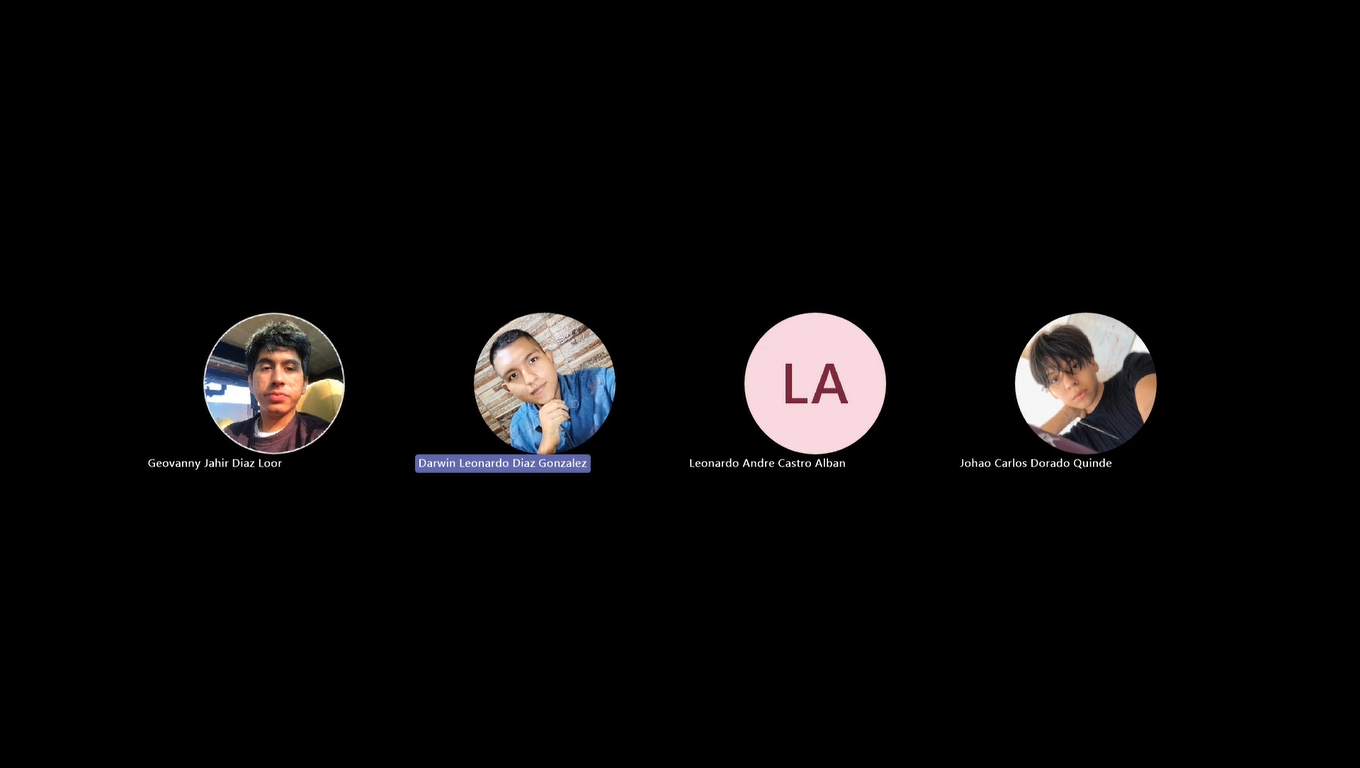
\includegraphics[width=0.85\textwidth]{ImgMeet1}
\caption{Product Owner Meeting 1 -- May 21}
\end{figure}

\begin{figure}[H]
\centering
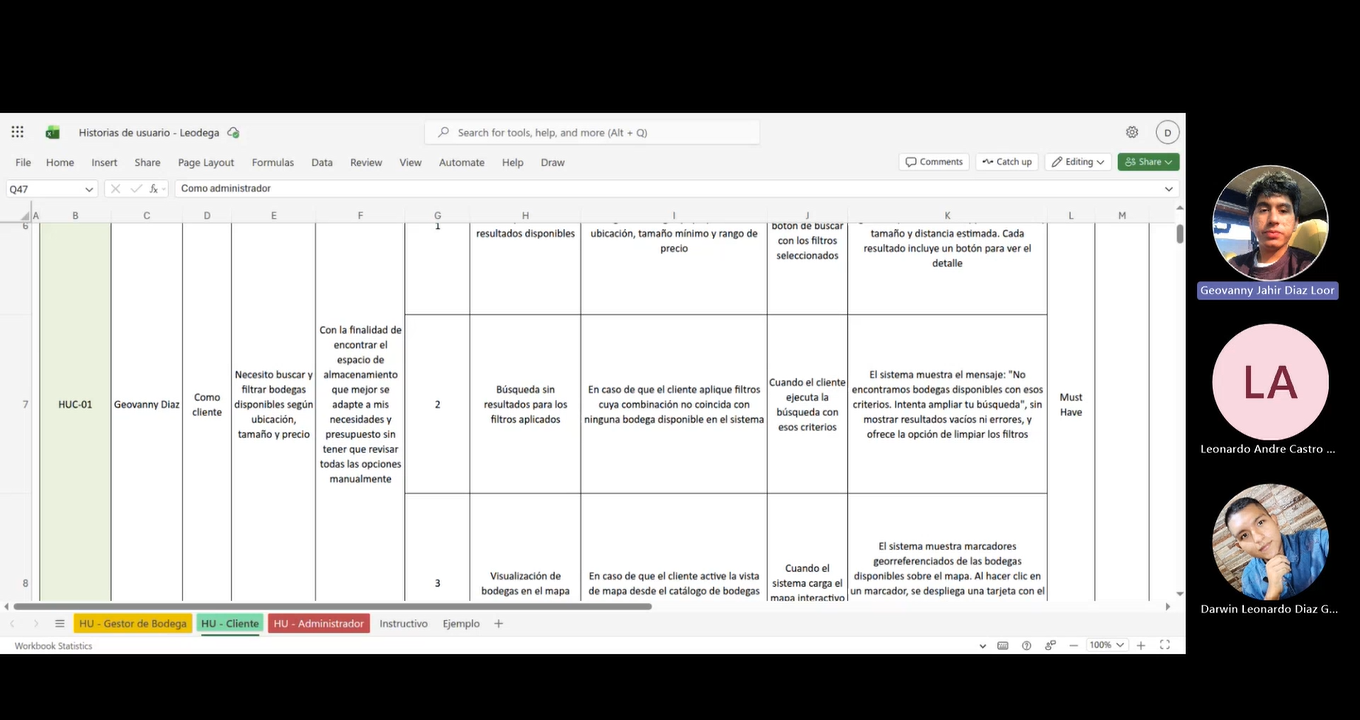
\includegraphics[width=0.85\textwidth]{ImgMeet2}
\caption{Product Owner Meeting 2 -- May 29}
\end{figure}

\begin{figure}[H]
\centering
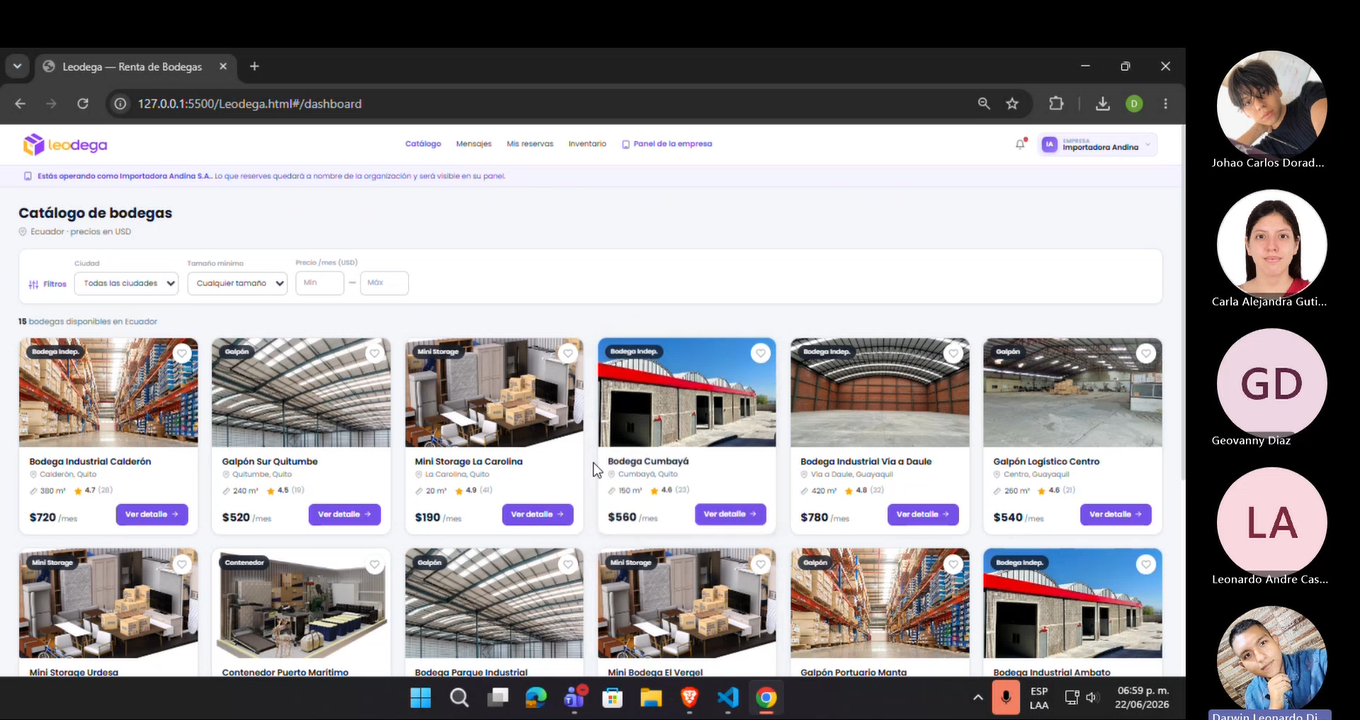
\includegraphics[width=0.85\textwidth]{ImgMeet3}
\caption{Product Owner Meeting 3 -- June 22}
\end{figure}

\end{document}
